\documentclass[a4paper,brazil,%
12pt,
%oldfontcommands,%
%showtrims,%
openright,
twoside,
%oneside
%draft
]{memoir}

\usepackage{bookpemd}
\usepackage{booktabs} % for much better looking tables
\usepackage{array} % for better arrays (eg matrices) in maths
\usepackage{paralist} % very flexible & customisable lists (eg. enumerate/itemize, etc.)
\usepackage{verbatim} % adds environment for commenting out blocks of text & for better verbatim
\usepackage{subfig} % make it possible to include more than one captioned figure/table in a single float
\usepackage{algpseudocode}
\usepackage{enumerate}
\usepackage{enumitem}
\usepackage{paralist} % very flexible & customisable lists (eg. enumerate/itemize, etc.)
\newcommand{\subscript}[2]{$#1 _ #2$}


%\usepackage{indentfirst}
%\usepackage{showkeys}

%\usepackage{makeidx}
%\makeindex

\includeonly{%
chapters/espaco_vetorial/main,%
chapters/subespacos_vetoriais/main,
chapters/combinacao_linear/main,
chapters/base_dimensao/main,
chapters/mudanca_base/main,
chapters/matriz_trans_linear/main,
chapters/transformacoes_lineares/main,
chapters/autovalores_autovetores/main,
chapters/espacos_produto_interno/main,
chapters/operadores_especiais/main,
}


%\overfullrule=5pt  % if a draft
\begin{document}
\frontmatter                            % only in book class (roman page #s)
{\contracapa{Notas de Aula de}{Álgebra Linear}
	{Volume I}
	{Lino Marcos da Silva}
	{lino.silva@univasf.edu.br}}

\newpage
% {\copyr}

% {\fichacat}
\tableofcontents*
%\addcontentsline{toc}{chapter}{Sumário}
\mainmatter                             % only in book class (arabic page #s)
\frenchspacing % remover espaço extra

\chapter{Espaço  Vetorial}
\thispagestyle{empty}

\section{Introdução}
\textit{Vetores} são entes matemáticos que se caracterizam por  possuir uma  intensidade,uma direção e um sentido. São utilizados, por exemplo, para representar grandezas físicas, como força e velocidade. No curso de Álgebra Linear, consideramos como  um vetor cada um dos  elementos de um   espaço vetorial.  No  contexto de espaços vetoriais, denominaremos de  \textit{escalar} qualquer elemento de um corpo\footnote{Corpo é uma estrutura matemática na qual está definida duas operações satisfazendo algumas propriedades} $\mathbb{K}$.  Nesse curso, iremos considerar $\mathbb{K}= \mathbb{R}$ (o corpo dos números reais) ou $\mathbb{K}=\mathbb{C}$ (o corpo dos números complexos).  A seguir daremos a definição de um espaço vetorial e apresentaremos alguns exemplos clássicos. Para alguns desses exemplos iremos apresentar a  prova,  de que os  mesmos  são espaços vetoriais,  na sala de aula; para alguns outros as provas serão apresentadas nesse texto e os demais ficarão como exercício para o aluno.   \textbf{Atenção.} \textit{Estas notas de aulas tem como objetivo guiar os alunos nos  estudos da disciplina álgebra linear, nas turmas de minha responsabilidade, nos cursos de engenharia da UNIVASF. O uso das mesmas  não dispensa  a leitura  dos livros didáticos indicados nas referências bibliográficas da disciplina, bem como a resolução de exercícios propostos nos mesmos}.

\section{Espaço Vetorial }

\textit{\textbf{Definição.}} Um conjunto $ V$  não vazio é um espaço vetorial sobre o corpo $\mathbb{K}$  se  em seus elementos,  denominados \textbf{vetores}, estiverem definidas as seguintes duas operações:
\begin{itemize}
\item \textbf{Soma de Vetores:} A  cada par   de elementos $u$ e $v$ de $V$ corresponde um vetor  $u+v$, chamado de soma de  $u$ e $v$, satisfazendo,  para quais quer $u$, $v$ e $w$ pertecentes a $V$, as seguintes propriedades:

\begin{enumerate}[label=(\subscript{A}{\arabic*})]
    \item $u+v=v+u$  (\textit{comutatividade})
    \item $u+(v+w)=(u+v)+w$  (\textit{associatividade})
    \item Existe um vetor $\theta \in V$,  denominado \textbf{vetor nulo}, tal que $u+\theta = u$.  (\textit{existência  do elemento neutro})
   \item Dado o vetor $u\in V$ existe o vetor $-u \in V$, denominado \textbf{vetor oposto}, tal que $u+(-u)=\theta$. (\textit{existência  do elemento simétrico})
    \end{enumerate}

 \item \textbf{Multiplicação por Escalar:}   A cada par $\alpha \in \mathbb{K}$   e  $v \in V$, corresponde um vetor $\alpha \times v$ , denominado produto por escalar de $\alpha$  por   $V$,  satisfazendo as seguintes propriedades:

\begin{enumerate}[label=(\subscript{ME}{\arabic*})]
     \item $\alpha \times (u+v)=\alpha \times u+\alpha \times v$
     \item$(\alpha + \beta) \times u= \alpha \times u+\beta \times u$
    \item $(\alpha \times \beta) \times u= \alpha (\beta \times u)$
   \item $1 \times u=u$.
    \end{enumerate}
\end{itemize}

Na definição anterior, quando $\mathbb{K}= \mathbb{R}$  dizemos que $V$ é um espaço vetorial real. Por outro lado, se $\mathbb{K}= \mathbb{C}$,   dizemos que $V$ é um espaço vetorial  complexo. Em um espaço vetorial $V$, o elemento neutro e o elemento oposto, das propriedades (A3) e (A4), respectivamente,  quando existem, são únicos.

\section{Exemplos}
\begin{enumerate}

\item \textbf{Espaço Vetorial Euclidiano.} O conjunto $\mathbb{R}^2=\{(x_1, x_2); x_i \in \mathbb{R}\}$ com as operações usuais de  soma de vetores $$(x_1, x_2)+(y_1, y_2)=(x_1+y_1, x_2+y_2)$$ e a multiplicação por escalar $$\alpha  (x_1, x_2)=(\alpha x_1, \alpha x_2)$$
é um espaço vetorial real.



\item O conjunto $\mathbb{R}^3=\{(x_1, x_2, x_3); x_i \in \mathbb{R}\}$ com as operações usuais de  soma de vetores $$(x_1, x_2, x_3)+(y_1, y_2, y_3)=(x_1+y_1, x_2+y_2, x_3+y_3)$$ e a multiplicação por escalar $$\alpha  (x_1, x_2, x_3)=(\alpha x_1, \alpha x_2, \alpha x_3)$$
é um espaço vetorial real.

\item De um modo geral para $n \geq 1$,  o conjunto $\mathbb{R}^n=\{(x_1, x_2,...,  x_n); x_i \in \mathbb{R}\}$ com as operações usuais de  soma de vetores $$(x_1, x_2,..., x_n)+(y_1, y_2,...,  y_n)=(x_1+y_1, x_2+y_2,..., x_n+y_n)$$ e a multiplicação por escalar $$\alpha  (x_1, x_2,..., x_n)=(\alpha x_1, \alpha x_2,..., \alpha x_n)$$
é um espaço vetorial real.

Dessa forma,  o  conjunto $\mathbb{R}$ com as operações de adição e multiplicação de números reais, onde nesse caso os vetores  são os números reais, é um espaço vetorial real  (Justifique).

\item \textbf{Espaço Vetorial de Matrizes.} O Conjunto $\mathbb{M}(m,n)$ das matrizes reais de ordem $m \times n$ com a soma  de matrizes e a multiplicação por escalar usuais  é um espaço vetorial real.

\item \textbf{Espaço Vetorial de Polinômios.} O conjunto de polinômios  $\mathbb{P}_n(t)=\{a_nt^n+a_{n-1}t^{n-1}+...+a_2t^2+a_1t+a_0,  \; \; a_i \in \mathbb{R}\}$    com as operações usuais de soma de polinômios
\begin{align*}
p(t)+q(t)&=(a_nt^n+ a_{n-1}t^{n-1}+...+a_1t_+a_0)+(b_nt^n+ b_{n-1}t^{n-1}+...+b_1t + b_0)\\
               &=(a_n+b_n)t^n+(a_{n-1}+b_{n-1})t^{n-1}+...+(a_1+b_1)t+a_0+b_0;
\end{align*}

 e multiplicação de polinômios por escalar
\begin{align*}
\alpha \cdot   p(t)&=(\alpha a_n)t^n+(\alpha a_{n-1})t^{n-1}+...+(\alpha a_1)t+\alpha a_0;
\end{align*}


é um espaço vetorial sobre $\mathbb{R}$.  Em particular,  o conjunto $$\mathbb{P}_2(t)=\{a_2t^2+a_1t+a_0,\; \;\text{com}\; \;  a_2, a_1 \;\; \text{e}\;\; a_0  \in \mathbb{R}\}$$   é um espaço vetorial, relativamente às mesmas operações. A seguir mostraremos que, de fato, $\mathbb{P}_2(t)$ é um espaço vetorial sobre $\mathbb{R}$.

\textbf{\textit{Demonstração.}}  Sejam $p(t)=a_2t^2+a_1t+a_0$, $q(t)=b_2t^2+b_1t+b_0$ e $m(t)=c_2t^2+c_1t+c_0$ elementos de $\mathbb{P}_2(t)$ e considere $\alpha , \beta \in \mathbb{R}$. Vamos mostrar que as operações soma de polinômios e multiplicação de polinômio por escalar possuem  as oitos propriedades da definição de espaço vetorial.

Primeiro vamos verificar que a propriedade (A1) é válida.  De fato,
\begin{align*}
p(t)+q(t)&=a_2t^2+a_1t+a_0+b_2t^2+b_1t+b_0\\
               &=(a_2+b_2)t^2+(a_1+b_1)t+(a_0+b_0)\\
               &=(b_2+a_2)t^2+(b_1+a_1)t+(b_0+a_0)\\
               &=q(t)+p(t)
\end{align*}
para todo $p(t), q(t) \in  \mathbb{P}_2(t)$. Agora, para mostrar que (A2) também vale, veja que
\begin{align*}
(p(t)+q(t))+m(t)&=(a_2+b_2)t^2+(a_1+b_1)t+(a_0+b_0)+c_2t^2+c_1t+c_0\\
               &=(a_2+b_2+c_2)t^2+(a_1+b_1+c_1)t+(a_0+b_0+c_0)\\
               &=(a_2+(b_2+c_2))t^2+(a_1+(b_1+c_1))t+(a_0+(b_0+c_0))\\
               &=\underbrace{a_2t^2+a_1t+a_0}_{p(t)} + (\underbrace{(b_2+c_2)t^2+(b_1+c_1)t+b_0+c_0}_{q(t)+m(t)})\\
               &=p(t)+(q(t)+m(t)).
\end{align*} Isto é, a soma de polinômios é \textbf{associativa}.

O \textit{polinômio identicamente nulo} de grau menor ou igual  a 2, $$\theta(t)=0t^2+0t+0,$$   é tal que
\begin{align*}
p(t)+\theta(t)&=a_2t^2+a_1t+a_0+0t^2+0t+0\\
               &=(a_2+0)t^2+(a_1+0)t+(a_0+0)\\
               &=a_2t^2+a_1t+a_0\\
               &=p(t),
\end{align*}
para todo $p(t) \in \mathbb{P}_2(t)$.  Logo, o polinõmio identicamente $\theta(t)=0t^2+0t+0$ é o  elemento neutro da soma de polinômios em  $\mathbb{P}_2(t)$, e assim a propriedade (A3) também está verificada.

Agora note, que para cada polinômio $p(t)=a_2t^2+a_1t+a_0 \in \mathbb{P}_2(t)$, existe o polinômio $-p(t)=-a_2t^2-a_1t-a_0 \in \mathbb{P}_2(t)$ tal que
\begin{align*}
p(t)+(-p(t))&=a_2t^2+a_1t+a_0+( -a_2t^2-a_1t-a_0\\
               &=(a_2-a_2)t^2+(a_1-a_1)t+(a_0-a_0)\\
               &=0t^2+0t+0\\
               &=\theta (t).
\end{align*}
Logo, a propriedade (A4) também está verificada.

Agora, para verificarmos a validade das propriedades (ME1)-(ME4), veja que para todo $\alpha, \beta \in \mathbb{R}$ e para todo $p(t), q(t)$ em $\mathbb{P}_2(t)$, temos:
\begin{align*}
\alpha(\beta (p(t)))&=\alpha( \beta (a_2t^2+a_1t+a_0))\\
               &=\alpha( \beta a_2t^2+\beta a_1t+\beta a_0)\\
               &=\alpha \beta a_2t^2+\alpha \beta a_1t+\alpha \beta a_0\\
               &=(\alpha \beta )(a_2t^2+ a_1t+ a_0)\\
               &=(\alpha \beta )p(t)
\end{align*}
e dessa forma, (ME1) é válida. Por outro lado,
\begin{align*}
(\alpha+\beta) p(t)&=(\alpha+\beta) (a_2t^2+a_1t+a_0)\\
               &=(\alpha+\beta)a_2t^2+(\alpha+\beta) a_1t+(\alpha+\beta) a_0\\
              &= \alpha a_2t^2+ \alpha a_1t+\alpha a_0  +\beta a_2t^2+\beta a_1t+\beta a_0\\
               &= \alpha (a_2t^2+  a_1t+ a_0 )+\beta (a_2t^2+ a_1t+ a_0)\\
               &=\alpha p(t)+ \beta p(t),
\end{align*}
e assim, (M2) é válida. Para mostrar que (ME3) também é válida, fazemos:
\begin{align*}
\alpha(p(t)+q(t))&=\alpha((a_2+b_2)t^2+(a_1+b_1)t+(a_0+b_0))\\
               &=(\alpha a_2+\alpha b_2)t^2+(\alpha a_1+\alpha b_1)t+(\alpha a_0+\alpha b_0)\\
               &=\alpha a_2 t^2 + \alpha a_1t+ \alpha a_0 + \alpha b_2t^2+\alpha b_1t+ \alpha b_0\\
               &=\alpha ( a_2 t^2 + a_1t+ a_0 )+ \alpha ( b_2t^2+ b_1t+ b_0)\\
               &=\alpha q(t)+\alpha p(t).
\end{align*}

Finalmente,
\begin{align*}
1 \cdot p(t)&=1 \cdot (a_2t^2+a_1t+ a_0)\\
                  &=1 \cdot a_2t^2+ 1\cdot a_1t+ 1 \cdot a_0\\
                 &= a_2t^2+  a_1t+  a_0\\
                 &=p(t)
\end{align*}
para todo $p(t) \in \mathbb{P}_2(t)$. Logo, a propriedade $(ME4)$ também  é válida e, portanto, mostramos que $\mathbb{P}_2(t)$ é um espaço vetorial real.
\item \textbf{Espaço Vetorial de Funções.} Dados números reais  $a$ e $b$  com $a < b$, considere  o intervalo da reta  $\mathbb{X}=[a,b]$ (ou seja, $\mathbb{X}$ é um subconjunto de $\mathbb{R}$).  Denotemos por  $\mathbb{F}(\mathbb{X}, \mathbb{R})$ o  conjunto formado por todas as  funções reais com domínio $\mathbb{X}$ e imagens real.  Isto é, o  conjunto formado por todas as funções
$$f: \mathbb{X} \rightarrow \mathbb{R}. $$  Considerando em $\mathbb{F}(\mathbb{X}, \mathbb{R})$  as operações de soma de funções e multiplicação de função  por escalar, como   definidas a seguir:

$$(f+g)(x)=f(x)+g(x) \; \; \text{e} \;\; (\alpha g)(x)=\alpha g(x), $$

então $\mathbb{F}(\mathbb{X}, \mathbb{R})$ é um espaço vetorial real.

\textbf{\textit{Demonstração.}} Sejam $f$, $g$ e $h$ funções definidas em $\mathbb{X}$.  Como para todo $ x \in \mathbb{X}$, temos $$f(x)+g(x)=g(x)+f(x)$$ pois $f(x)$  e $g(x)$ sao números reais, então  temos $$(f+g)(x)=f(x)+g(x)=g(x)+f(x)=(g+f)(x),$$ para todo $ x \in \mathbb{X}$. Logo, $f+g=g+f$. Isto é, a soma de funções é \textbf{comutativa}.

De modo análogo,$$[f+(g+h)](x)=f(x)+(g+h)(x)=f(x)+g(x)+h(x)=(f+g)(x)+h(x)=[(f+g)+h](x),$$   para todo $ x \in \mathbb{X}$. Logo, $f+(g+h)=(f+g)+h$, e assim,  a soma de funções é \textbf{associativa}.

Existe a função $f: \mathbb{X} \rightarrow \mathbb{R}$,  tal que,  $f(x)=0$ para todo   $ x \in \mathbb{X}$. Trata-se da função \textit{nula}, que será denotada por $\theta$. Assim, para todo  $ x \in \mathbb{X}$ e para toda $f \in  \mathbb{F}(\mathbb{X}, \mathbb{R})$  temos $$ (\theta+f)(x)
=\theta(x)+f(x)=0+f(x)=f(x).$$ Ou seja, existe a função $\theta(x) \in \mathbb{F}(\mathbb{X}, \mathbb{R})$   tal que $$\theta + f=f$$ para toda $ f \in \mathbb{F}(\mathbb{X}, \mathbb{R})$. A função nula é o \textbf{ elemento neutro} desta operação.

Para cada função $f: \mathbb{X} \rightarrow \mathbb{R}$ dada, a função $-f: \mathbb{X} \rightarrow \mathbb{R}$, que transforma cada $ x \in \mathbb{X}$ em  $-f(x)$ é tal que
$$[f+(-f)](x)=f(x)+(-f(x))=0=\theta(x).$$  Logo, dada função $f \in \mathbb{F}(\mathbb{X}, \mathbb{R})$, existe a função $ -f \in  \mathbb{F}(\mathbb{X}, \mathbb{R})$ tal que $f+(-f)=\theta$.  Isto é, a função $-f$ é o \textbf{elemento simétrico} da soma de funções.

Agora sejam $\alpha,\beta \in \mathbb{R}$ e $f, g \in \mathbb{F}(\mathbb{X}, \mathbb{R})$.

$\alpha(\beta f)(x)=\alpha(\beta  f(x))=(\alpha\beta )f(x)$ para todo $ x \in \mathbb{X}$.  Logo, $$ \alpha(\beta  f)=(\alpha \beta )f.$$

$((\alpha+\beta )f)(x)=(\alpha+\beta )f(x)=\alpha f(x)+\beta f(x)=(\alpha f+\beta f)(x)$ para todo $ x \in \mathbb{X}$. Logo, $$ (\alpha+\beta)  f=\alpha f + \beta f.$$


$(\alpha(f+g))(x)=\alpha(f+g)(x)=\alpha (f(x)+g(x))=\alpha f(x)+\alpha g(x)=(\alpha f+\alpha g)(x)$  para todo $ x \in \mathbb{X}$. Logo, $$ \alpha ( f+g)=\alpha f + \alpha g.$$

Finalmente, $1\cdot f(x)= f(x)$ para todo $ x \in \mathbb{X}$. Logo, $$ 1 \cdot f= f.$$

Dessa forma, as operações de soma de funções e multiplicação por escalar satisfazem as oitos propriedades da definição, e portanto, $\in \mathbb{F}(\mathbb{X}, \mathbb{R})$ é um espaço vetorial sobre $\mathbb{R}$.

\item \textbf{Espaço Vetorial das Soluções de um Sistema Linear Homogêneo.} O conjunto $\{ (x_1, x_2, ..., x_n), x_i \in \mathbb{R}\}$ das soluções de um sistema linear homogêneo
 \begin{equation} \left\{
\begin{tabular}{lllllllllll}
$a_{11}x_1$ &+& $a_{12}x_2$ &+&\dots&+&$a_{1n}x_n$& $=$ & $0$ \\
$a_{21}x_1$ &+& $a_{22}x_2$ &+&\dots&+&$a_{2n}x_n$&$=$ & $0$ \\
.&&&&&&&& \\ .&&&&&&&& \\ .&&&&&&&& \\

$a_{m1}x_1$ &+& $a_{m2}x_2$ &+&\dots&+&$a_{mn}x_n$ &$=$ & $0$ \\
\end{tabular},  \right.\label{sist2}
\end{equation}
também é um espaço vetorial.

\end{enumerate}

\section{Exercícios Propostos}

\begin{enumerate}

\item  Seja $V$  o espaço vetorial  $\mathbb{R}^n$. Qual é o vetor nulo de$V$? O que representa o vetor $ – (x_1, x_2,...,x_n$)?

\item  Seja $W=\mathbb{M}(2,2)$. Descreva o vetor nulo e vetor oposto em $W$.

\item Descreva o vetor nulo e o vetor oposto em $\mathbb{P}_2(t)=\{a_2t^2+a_1t+a_0,\; \;\text{com}\; \;  a_i  \in \mathbb{R}\}$.

\item Mostre que o conjunto $V=\{ (x,y); x, y \in \mathbb{R} \; \; \text{e} \; \; xy> 0\}$ com as operações $$ (a,b) \oplus + (c,d)= (ac, bd) \;\; \text{e} \;\; \alpha \otimes (a,b)=(a^{\alpha}, b^{\alpha})$$ é  um espaço vetorial real.

\item  Mostre que o conjunto $V=\{ (1,y);  y \in \mathbb{R}\}$ com as operações $$ (1,y_1) + (1,y_2)= (1, y_1+y_2) \;\; \text{e} \;\; \alpha  (1,y)=(1, {\alpha}y)$$ é  um espaço vetorial real.



\item Seja o conjunto $\mathbb{R}^2=\{(x, y); x, y  \in \mathbb{R}\}$. Mostre que $\mathbb{R}^2$ não é um espaço vetorial com as operações assim definidas:
$$ (x,y) + (z,w)= (x+z, y+w) \;\; \text{e} \;\; \alpha  (x,y)=({\alpha}x, y).$$

\item  Mostre a seguinte afirmação: Em um espaço vetorial $V$ existe um único vetor nulo e cada elemento de$V$ possui um único inverso.

\item Mostre que os exemplos 4 e 7 são de fato espaços vetoriais sobre $\mathbb{R}$.




\end{enumerate}

\chapter{Subespaços Vetoriais}
\thispagestyle{empty}

\section{Introdução}
Um espaço vetorial pode ser um conjunto muito grande e às vezes  pode ser útil identificar outros espaços vetoriais dentro dele. Espaços vetoriais que estão dentro de outros espaços vetoriais são chamados de subespaços vetoriais.   \textbf{Atenção.} \textit{Estas notas de aulas tem como objetivo guiar os alunos nos  estudos da disciplina álgebra linear, nas turmas de minha responsabilidade, nos cursos de engenharia da UNIVASF. O uso das mesmas  não dispensa  a leitura  dos livros didáticos indicados nas referências bibliográficas da disciplina, bem como a resolução de exercícios propostos nos mesmos}.

\section{Subespaço Vetorial}


\textbf{Definição.} Sejam $V$ um espaço vetorial e $ W$ um subconjunto  não vazio de $V$.  O subconjunto  $W$ é um \textbf{subespaço vetorial} de $V$,  se $W$ é um espaço vetorial  em relação as operações  de adição de vetores e multiplicação por escalar definidas em $V$.

\vspace{0.3cm}

De acordo com a definição anterior, qualquer subespaço de  um espaço vetorial  $V$ deve, necessariamente, conter o vetor nulo de $V$. De fato, a operação de adição de vetores a ser considerada no subconjunto $W$ é  obrigatoriamente a mesma de $V$ e o elemento neutro dessa operação é único.  A Figura \ref{fig:subespaco} ilustra esse fato.



\begin{figure}[h!]
\center
% \includegraphics[width=0.7\textwidth]{subespaco}
\caption{\footnotesize{Um subespaço vetorial é um espaço vetorial dentro de outro}}
\label{fig:subespaco}
\end{figure}


%\vspace{0.3cm}
Todo espaço vetorial $V$ admite pelo menos dois subespaços: o conjunto formado apenas pelo vetor nulo  e o próprio espaço. Isto é,  $\{ 0\}$ e  $V$. Esses dois subespaços de $V$  são chamados de \textbf{subespaços triviais}.

%\vspace{0.3cm}

Utilizar a definição de subespaço vetorial para  identificar se um subconjunto $W$  de um espaço vetorial $V$  é um subespaço é  uma atividade laboriosa, pois exige a verificação das oito propriedades,  (A1)-(A4) e (ME1)-(ME4), da definição de espaço vetorial. Felizmente, de acordo com a  próxima proposição,  não precisaremos fazer  a verificação de todas essas propriedades. De fato, sendo  $W$  um subconjunto de $V$,  as propriedades  das operações que são válidas em $V$ devem também ser válidas em $W$, desde que $W$ seja um conjunto fechado em relação a essas operações. Isto é, o resultado das operações realizadas com elementos de $W$  resultam em elementos de $W$.

 Um subespaço vetorial $W$ de um espaço vetorial $V$  fica caracterizado pela seguinte proposição:

\textbf{Proposição.} Dados um espaço vetorial $V$ e  um subconjunto $W$ de $V$   não vazio. $W$ é um subespaço de  $V$ se as duas condições a seguir  forem satisfeitas:

\begin{enumerate}[label=(\roman*)]
\item Se $u$ e $v$ são vetores quaisquer de $W$, então $u+v \in W$;
\item Se  $ \alpha \in \mathbb{R}$ e $ v$ é um vetor qualquer de $W$, então $\alpha v\in W$.

\end{enumerate}

\textbf{\textit{Observações.}}
\begin{enumerate}%[label=(\roman*)]
\item Todo subespaço $W$ de um espaço vetorial $V$ precisa, necessariamente, conter o vetor nulo de $V$. De fato, se tomarmos $\alpha=0$, por (ii),  temos $$0\cdot v=0 $$ para todo $v \in W$.

\item Dessa forma,  se um subconjunto não vazio  $W$ de um espaço vetorial $V$ não possuir o vetor nulo de $V$,  então $W$ não pode ser um subespaço vetorial de $V$.
\end{enumerate}

\section{Exemplos}
\begin{enumerate}


\item Seja $V=\mathbb{R}^2=\{(x_1, x_2); x_i \in \mathbb{R}\}$ com as operações usuais de  soma de vetores e a multiplicação por escalar.  O subconjunto
$$W=\{(x, y); y=kx, \; \text{$k$ é uma constante} \}$$ é um subespaço vetorial de $V$.

\textbf{\textit{Demonstração.}}
Observe que $W$ também pode ser escrito da seguinte maneira:
$$W=\{(x, kx);  x \in \mathbb{R} \; \text{e}\; \text{$k$ constante} \}.$$   Primeiro é conveniente observar que $(0,0) \in W$. De fato, para $x=0$ teremos $kx=0$, para todo $k\in \mathbb{R}$. Logo, $(0,0) \in W$ e, desse modo, $W \neq \emptyset$.

Agora sejam $u=(x_1, y_1)$ e $v=(x_2, y_2)$ vetores de $W$.  Dessa maneira, podemos escrever $u=(x_1, kx_1)$ e $v=(x_2, kx_2)$. Assim,
\begin{align*}
u+v &=(x_1, kx_1)+(x_2, kx_2)\\
       &=(x_1+x_2, kx_1+kx_2)\\
       &=(x_1+x_2, k(x_1+x_2)).
\end{align*}
Fazendo $x_3=x_1+x_2$, temos que $u+v =(x_3, kx_3)$. Logo, $u+v \in W$ e o item (i) é satisfeito.  Agora seja  $\alpha \in \mathbb{R}$ e $u=(x_1, y_1) \in W$. Assim
\begin{align*}
\alpha u &=\alpha(x_1,x_2)\\
            &=\alpha (x_1, kx_1) \; \text{pois} \;  u \in W;\\
       &=(\alpha x_1, \alpha k x_1).
\end{align*}
 Fazendo $x_4=\alpha x_1$ temos que $\alpha u=(x_4, kx_4)$. Logo, $\alpha u \in W$ e o intem (ii) da proposição está satisfeito.  Poranto, $W$ é um subespaço vetorial de $V$. Observe ainda que os elementos de  $W$ descrevem uma reta passando pela origem.

\item Seja $V=\mathbb{R}^2$ e $U=\{(x, 5x+3);  x \in \mathbb{R}\}$.  O subconjunto $U$,  com as operações usuais de  soma de vetores e a multiplicação por escalar,não é um subespaço vetorial de $\mathbb{R}^2$.   De fato,  o vetor $\{(0,0\}$ não pertence a $W$. Observe que os elementos de $U$ descrevem uma reta em $\mathbb{R}^2$ que não passa pela origem.


\item Todos os subespaços de $\mathbb{R}^2$ são:  $\{(0,0)\}$, o  $\mathbb{R}^2$  e os seus subconjuntos que descrevem  retas passando pela origem.

\item Seja $W=\{(x,y,z) \in \mathbb{R}^3; ax+by+cz=0\}$.  Observe que $W$ descreve, em $\mathbb{R}^3$, um \textbf{plano que passa pela origem}.  $W$ é um subespaço vetorial de $\mathbb{R}^3$.

\textbf{\textit{Demonstração.}}
  Primeiro é conveniente observar que $(0,0,0) \in W$. De fato, para $x=y=z=0$ teremos $ax+by+cz=0$, quaisquer que sejam os escalares  $a,b,c \in \mathbb{R}$. Logo, $(0,0,0) \in W$ e, desse modo, $W \neq \emptyset$.

Agora sejam $u=(x_1, y_1, z_1)$ e $v=(x_2, y_2, z_2)$ vetores de $W$.  Dessa maneira,  temos que $ax_1+bx_1+cz_1=0$ e  $ax_2+bx_2+c_z2=0$. Assim,  temos
\begin{align*}
u+v &=(x_1, y_1, z_1)+(x_2, y_2, z_2)\\
       &=(x_1+x_2, y_1+y_2, z_1+z_2).
\end{align*}
Fazendo $x_3=x_1+x_2$,$y_3=y_1+y_2$ e $z_3=z_1+z_2$ temos que
\begin{align*}
ax_3+by_3+cz_3&=a(x_1+x_2)+b(y_1+y_2)+c(z_1+z_2)\\
                             &=\underbrace{ax_1+by_1+cz_1}_{0}+\underbrace{ax_2+by_2+cz_2}_{0}\\
                             &=0+0=0.
\end{align*}
Logo, $u+v  \in W$ e o item (i) é satisfeito.  Agora seja  $\alpha \in \mathbb{R}$ e $u=(x_1, y_1, z_1) \in W$. Assim, $ax_1+bx_1+cz_1=0$.
\begin{align*}
\alpha u &=\alpha(x_1,y_1, z_1)\\
            &=\alpha (x_1,y_1, z_1) \\
       &=(\alpha x_1, \alpha y_1, \alpha z_1).
\end{align*}
 Fazendo $x_4=\alpha x_1$, $y_4=\alpha y_1$ e  $z_4=\alpha z_1$ temos que
\begin{align*}
ax_4+by_4+cz_4&=a(\alpha x_1)+b(\alpha y_1)+c(\alpha z_1)\\
                              &=\alpha ( ax_1 +b y_1+cz_1)\\
                             &=\alpha\underbrace{ax_1+by_1+cz_1}_{0}\\
                             &=\alpha \cdot 0=0.
\end{align*}
Logo, $\alpha u \in W$ e o intem (ii) da proposição está satisfeito.  Portanto, $W$ é um subespaço vetorial de $\mathbb{R}^3$.


\item Todos os subespaços de $\mathbb{R}^3$ são:  $\{(0,0,0)\}$, o  $\mathbb{R}^3$, os seus subconjuntos que descrevem  retas passando pela origem e os subconjuntos que descrevem planos passando pela origem.


\item Considere em $\mathbb{M}(n,n)$  o conjunto $S$ das matrizes simétricas de ordem $n$.  $S$ é um subespaço vetorial de $\mathbb{M}(n,n)$ . Isto é, $$S=\{ A \in \mathbb{M}(n,n); A^T=A\}.$$ $S$ é um subespaço vetorial de $\mathbb{M}(n,n)$ .

\textbf{\textit{Demonstração.}}
Primeiro observe que a matriz nula de ordem $n$ é uma matriz simétrica. Logo, $ S \neq \emptyset$.  Agora sejam $A$ e $B$ matrizes simétricas de ordem $n$. Pela propriedade das matrizes  simétricas, temos que $$ (A+B)^T=A^T+B^T. $$
Por outro lado, $A$ e $B$ são matrizes simétricas. Logo, $A^T=A$ e $B^T=B$. Daí, vem que  $$ (A+B)^T=A^T+B^T = A +B .$$ Ou seja, $A+B$ é uma matriz simétrica. Logo, $A+B \in  \mathbb{M}(n,n)$.

Dado $\alpha \in \mathbb{R}$ e $A$ uma matriz simétrica de ordem $n$, temos, pela propriedade de matriz simétrica, que  $$(\alpha A)^T= \alpha A^T=\alpha A.$$ Assim, $\alpha A$ é uma matriz simétrica, ou seja, $\alpha A \in \mathbb{M}(n,n)$. Portanto, $S$ é um subespaço vetorial de $\mathbb{M}(n,n)$.


\item Considere o sistema linear homogêneo $$AX=0$$ onde  $A$, a matriz dos coeficientes, tem  ordem $m \times n$, $X$ é a matriz das incógnitas  e tem ordem $n \times 1$ e $0$ pé matriz dos termos independentes e tem ordem $ m \times 1$.  Seja $S_h$ o conjunto das soluções desse sistema linear homogêo.  Isto é,
$$S_h=\{ X \in \mathbb{M}(n,1); AX=0 \}.$$  $S_h$ é um subespaço vetorial de $\mathbb{M}(n,n)$ .
\end{enumerate}

\subsection{Intersecção de Subespaços}
Seja  $V$ um espaço vetorial sobre um corpo $\mathbb{K}$. Suponha que $U$ e $W$ são  subespaços vetoriais de $V$. Então o conjunto
$$U\cap W=\{ v \in V;  \; v \in U \; \text{e} \; v \in W \} $$ é um subespaço vetorial de $V$.

\textbf{\textit{Demonstração.}}

Primeiro note que $U\cap W \neq \emptyset$. Isto é, $0 \in U\cap W$. De fato,  como $U$ e $W$ são subespaços de $V$, então $0 \in U$ e $0 \in W$, logo $0 \in U\cap W$.

Agora, vamos mostrar que a soma de dois vetores quaisquer de $U \cap W$ é um vetor de  $U \cap W$.  Para isso suponha que $u,v \in U\cap W$. Dessa forma temos:
\begin{align*}
u\in U\cap W&, \; \text{ logo $u \in U$ e $u \in W$};\\
v\in U\cap W &, \; \text{logo  $v \in U$ e $v \in W$}.
\end{align*}
Dessa maneira, temos  $u, v \in U$;   e $u,v \in W$. Como $U$ e $W$ são subespaços, então $u+ v \in U$  e $u+v \in W$. Logo, $$u+ v \in U \cap W. $$

Para mostrarmos que a multiplicação de um vetor de $U\cap W$ por um escalar  também é um vetor $U\cap W$,  considere $\alpha \in \mathbb{K}$  e $u \in U\cap W$.  Desse modo,  $u\in U$ e $u \in W$  (ambos são subespaços de $V$), então   $\alpha \cdot  u \in U$ e $\alpha \cdot  u \in W$.
Logo, $\alpha \cdot  u\in U\cap W$. Dessa forma concluimos que $U\cap W$ é um subespaço vetorial de $V$.

\subsubsection{\textbf{Exemplos}}
\begin{enumerate}
\item Considere os subespaços de $\mathbb{R}^3$
$$ U= \{(x,y,z) \in \mathbb{R}^3 ; z=0\} $$ e  $$ W= \{(x,y,z) \in \mathbb{R}^3 ; x=0\}.  $$ Seja $(a, b, c)$ um vetor qualquer de $\mathbb{R}^3$. Observe que  $(a, b,c ) \in U\cap W$ se, e somente se,  $(a, b, c) \in U$ e $(a, b, c) \in W$, simultaneamente. Mas, isso somente ocorre se tivermos  $a=0$   e $c=0$. Logo, um  vetor $v$ do $\mathbb{R}^3$ está em $U \cap W$ se, e somente se, $v$ é do tipo $(0, b, 0)$. Assim, escrevemos $$U \cap W=\{(x, y, z) \in\mathbb{R}^3; x=z=0 \}=\{ (0,y,0); y \in \mathbb{R}\}.$$


\item Considere em $\mathbb{R}^2$ os subespaços
$$ U= \{(x,y) \in \mathbb{R}^2 ; y=x\} $$ e  $$ W= \{(x,y) \in \mathbb{R}^2 ; y=-x\}.  $$ Seja $(a, b)$ um vetor qualquer de $\mathbb{R}^2$. Observe que  $(a, b ) \in U\cap W$ se, e somente se,  $(a, b) \in U$ e $(a, b) \in W$, simultaneamente. Mas, isso ocorre somente  se tivermos  $b=a$   e $b=-a$. De onde concluímos que $b=0$ e $a=0$.  Logo, um  vetor $v$ do $\mathbb{R}^2$ está em $U \cap W$ se, e somente se, $v=(0, 0)$. Assim, obtemos $$U \cap W=\{(0,0) \}.$$

\item  Sejam $V= \mathbb{M}(n,n)$ seja o espaço vetorial  das matrizes quadradas, com entradas reais,  de ordem $n$; $U$ o subconjunto  das matrizes triangulares inferiores e $W$ o subconjunto das matrizes triangulares superiores de ordem $n$.  É possível mostrar que $U$ e $W$ são subespaços vetoriais de $V$ (Exercício).  Observe que $U \cap W$ é o conjunto de todas as matrizes diagonais de ordem $n$.
\end{enumerate}

Sobre a reunião, $U \cup W$, de dois subespaços $U$ e $W$ de um dado espaço vetorial $V$ podemos dizer que, em geral, não é um subespaço vetorial de $V$. A Figura \ref{fig:intersect} ilustra a união e a intersecção de subconjuntos de $V$.

\begin{figure}[h!]
	\center
	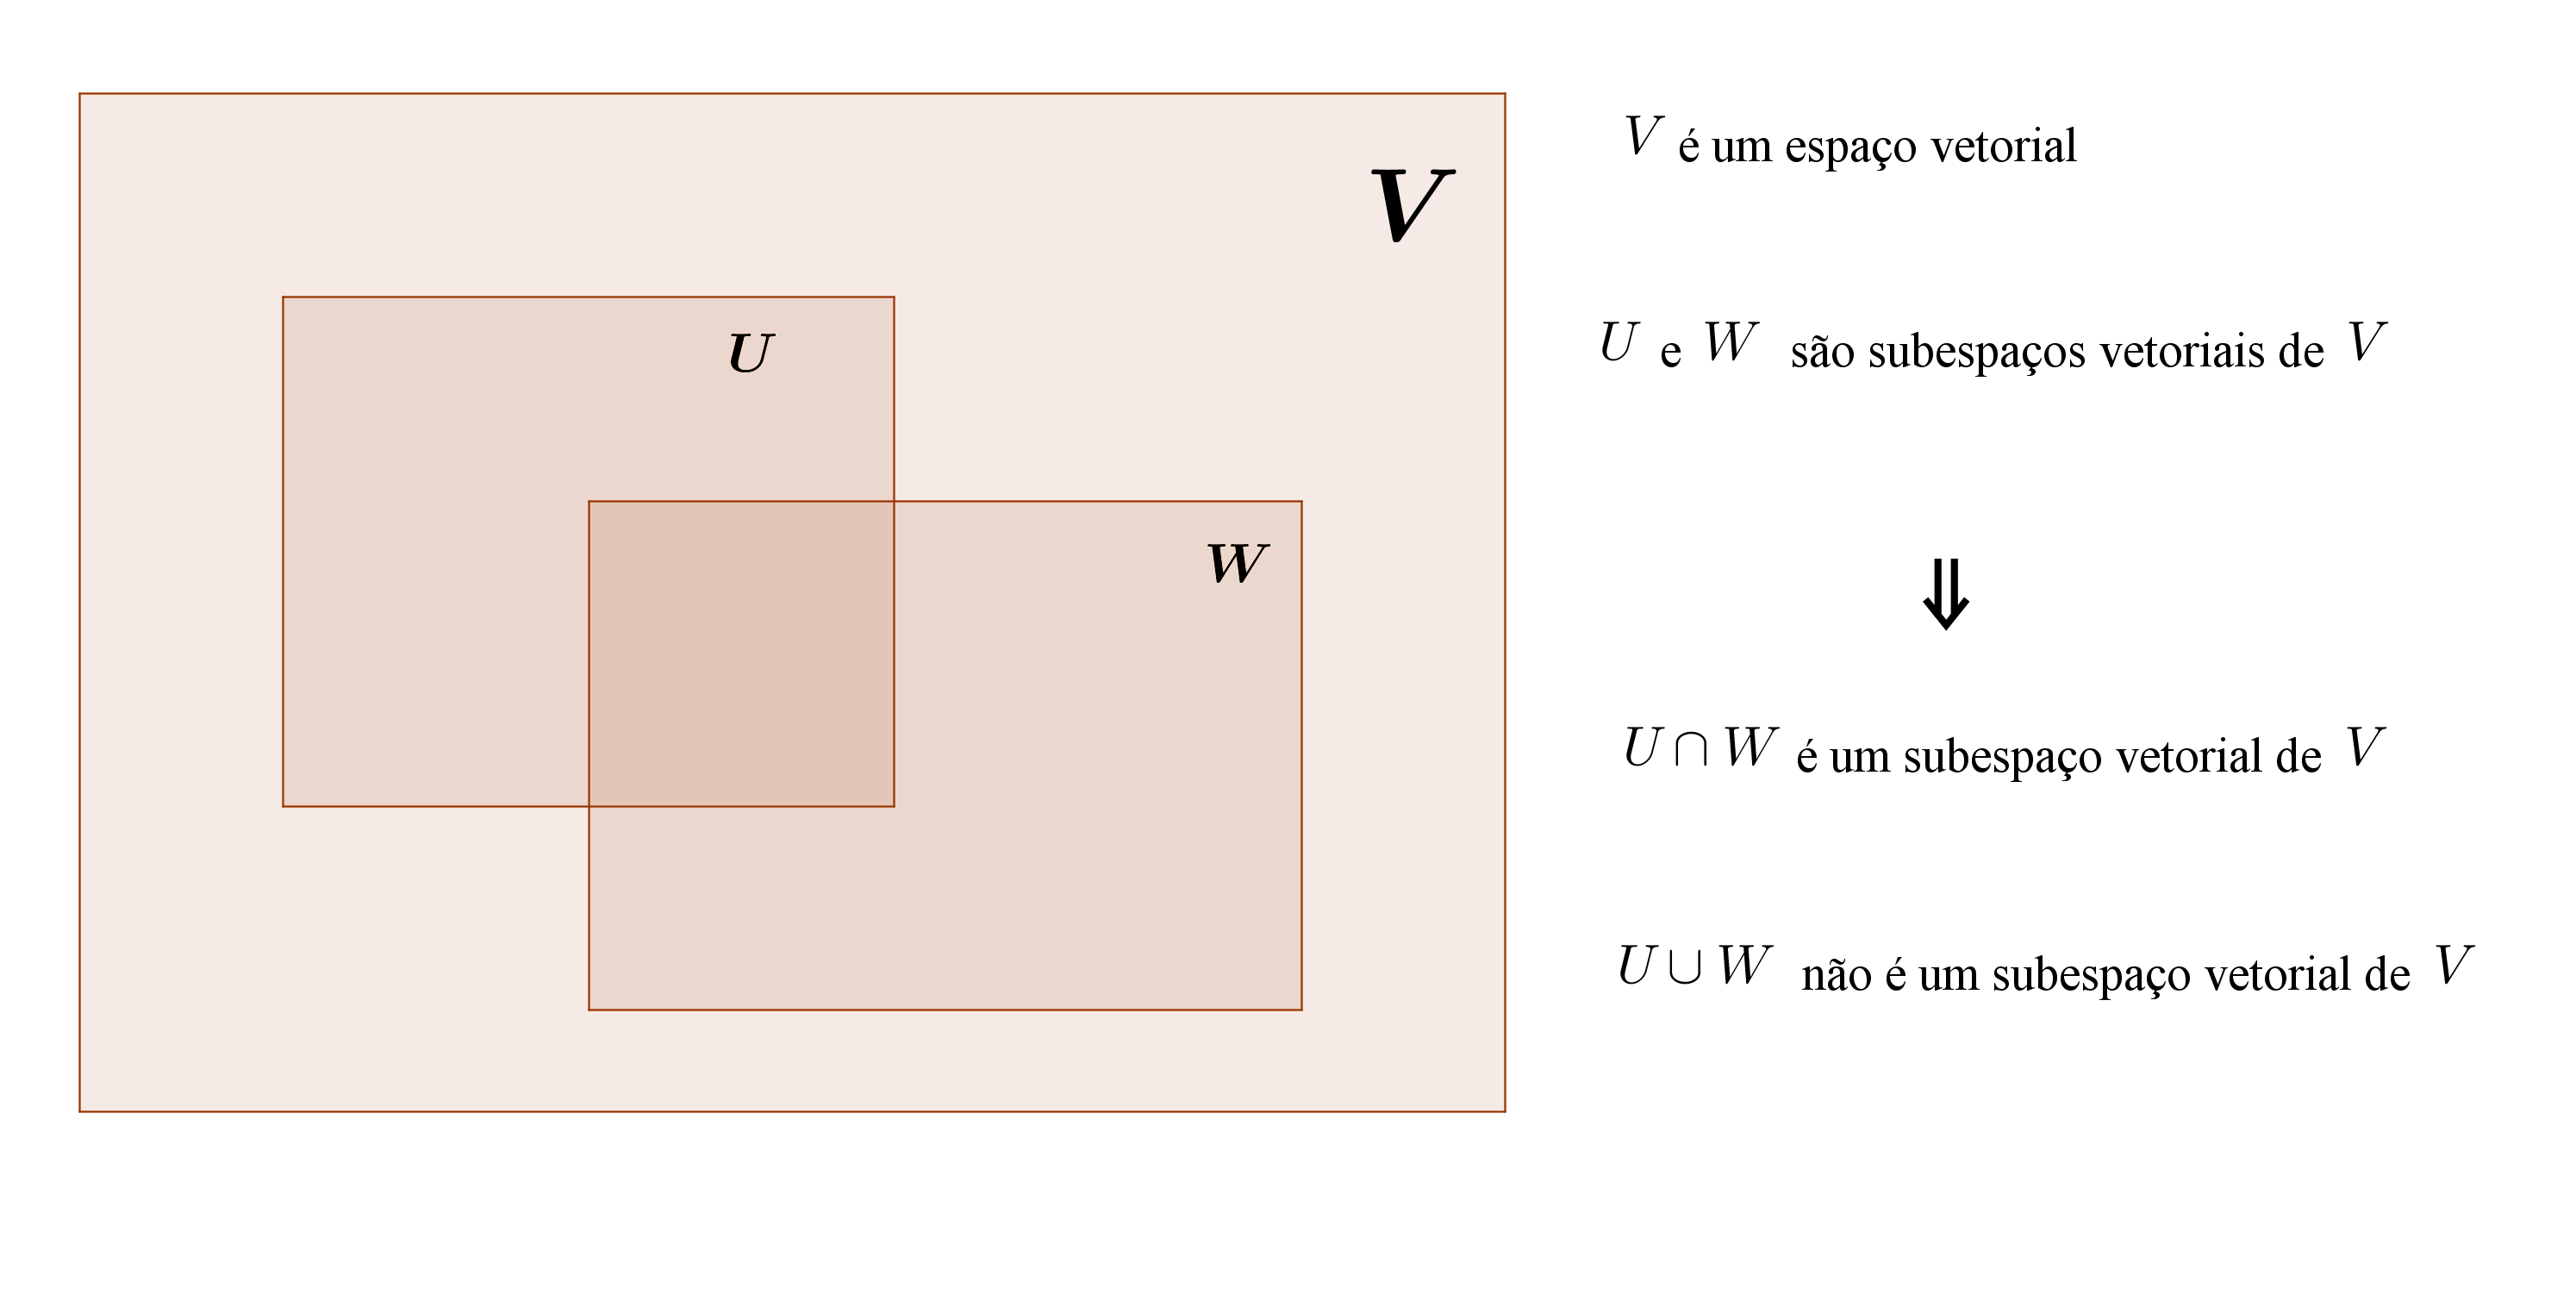
\includegraphics[width=0.7\textwidth]{chapters/subespacos_vetoriais/img/intersect}
	\caption{\footnotesize{A intersecção de subespaços vetoriais é um subespaço vetorial}}
	\label{fig:intersect}
\end{figure}

Mostraremos que a reunião de dois subespaços nem sempre é um subespaço vetorial, apresentando um exemplo no espaço vetorial $\mathbb{R}^2$. Considere os seguintes subespaços vetoriais de $\mathbb{R}^2$:  $$U=\{(x, 0); x \in \mathbb{R}\} \;\;\text{e} \;\;  W=\{(0, y); y \in \mathbb{R} \}.$$ Observe que o vetor $(2,0) \in U$  e o vetor $(0,5) \in W$. Logo, ambos pertencem ao conjunto  $U \cup W$. No entanto, a soma desses dois vetores $$(2,0)+(0,5)=(2,5)$$ não é um vetor de $U$ nem um vetor $W$. Logo, não é um vetor de $U \cup W$. Portanto, $U \cup W$ não é um subespaço vetorial de $\mathbb{R}^2$.







\subsection{Soma de Subespaços}
Seja  $V$ um espaço vetorial sobre um corpo $\mathbb{K}$. Suponha que $U$ e $W$ são  subespaços vetoriais de $V$. Então o conjunto
$$U+W=\{ v \in V; v=v_1+v_2, \; v_1 \in U \; \text{e} \; v_2 \in W \} $$ é um subespaço vetorial de $V$. O subespaço $U+W$ chama-se \textit{ soma} de $U$ e $W$.

\textbf{\textit{Demonstração.}}

Primeiro note que $U+W \neq \emptyset$. Isto é, $0 \in U+W$. De fato,  como $U$ e $W$ são subespaços de $V$, $0 \in U$ e $0 \in W$. Desse modo, como  $$0=0+0,$$ temos que $0$ pode ser escrito como a soma de um elemento de $U$ com um elemento de $W$.

Sejam $u,v \in U+W$. Dessa forma podemos escrever
\begin{align*}
u&=u_1+w_1, \; \text{com $u_1 \in U$ e $w_1 \in W$};\\
v&=u_2+w_2, \; \text{com $u_2\in U$ e $w_2 \in W$}.
\end{align*}
Assim, como $u_1, u_2 \in U$ (e $U$ é um subespaço de $V$), então $u_1+u_2 \in U$.  Do mesmo modo, como $w_1, w_2 \in W$ (e $W$ é um subespaço de $V$), então $w_1+w_2 \in W$.

Desse modo,
\begin{align*}
u+v&=(u_1+w_1) + (u_2+w_2) \\
         &=(u_1+u_2)+(w_1+w_2).
\end{align*}
Fazendo $u_3=u_1+u_2$ e $w_3=w_1+w_2$, temos que $u+v=u_3+w_3$, onde $u_3 \in U$ e $w_3 \in W$. Logo, $u+v \in U+W$.

Agora, sejam $\alpha \in \mathbb{K}$  e $u \in U+W$.  Logo, existem $u_1 \in U$ e $w_1 \in W$ tais que $u=u_1+w_1$. Daí,
\begin{align*}
\alpha \cdot  u&=\alpha \cdot (u_1+w_1) \\
         &=\alpha \cdot  u_1+\alpha \cdot  w_1.
\end{align*}
Note que $\alpha \cdot  u_1 \in U$ e $\alpha \cdot  w_1 \in W$, pois $U$ e $W$ sao subespaços.  Assim, fazendo $u_4=\alpha \cdot  u_1$ e $w_4=\alpha \cdot  w_1$, temos que $\alpha \cdot  u=u_4+w_4$, onde $u_4 \in U$ e $w_4 \in W$. Logo, $\alpha \cdot  u\in U+W$. Dessa forma concluimos que $U+W$ é um subespaço vetorial de $V$.

\subsubsection{\textbf{Exemplos}}
\begin{enumerate}
\item Considere em  $\mathbb{R}^3$, os subespaços
$$ U= \{(x,y,z) \in \mathbb{R}^3 ; z=0\} $$ e  $$ W= \{(x,y,z) \in \mathbb{R}^3 ; x=y=0\}.  $$ Dado   $(a, b, c)$ um vetor qualquer de $\mathbb{R}^3$, podemos escrever
$$(a, b, c)= (a,b,0)+(0,0,c).$$

 Observe que  $(a, b,0 ) \in U$ e  $(0, 0, c) \in W$. Logo, $(a,b,c) \in U+W$.  Como $(a,b,c)$ é um vetor arbitrário de $\mathbb{R}^3$, concluimos que $$U+W=\mathbb{R}^3.$$


\item Considere em $\mathbb{R}^2$, os subespaços
$$ U= \{(x,y) \in \mathbb{R}^2 ; y=x\} $$ e  $$ W= \{(x,y) \in \mathbb{R}^2 ; y=-x\}.  $$ Seja $(a, b)$ um vetor qualquer de $\mathbb{R}^2$.  Note que  podemos escrever
$(a, b)$ do seguinte modo: $$(a,b)=\left(\dfrac{a+b}{2},\dfrac{a+b}{2}   \right)+\left(\dfrac{a-b}{2},\dfrac{-a+b}{2}   \right).$$

Como $\left(\dfrac{a+b}{2},\dfrac{a+b}{2}   \right) \in U$ e $\left(\dfrac{a-b}{2},\dfrac{-a+b}{2}   \right) \in W$, então $(a,b) \in U+W$.  Mas, $(a,b)$ é um vetor arbitrário de $\mathbb{R}^2$, logo $$\mathbb{R}^2 = U+W.$$



\item  Sejam $V= \mathbb{M}(2,2)$ seja o espaço vetorial  das matrizes quadradas, com entradas reais,  de ordem $2$; $U$ o subconjunto  das matrizes triangulares inferiores e $W$ o subconjunto das matrizes triangulares superiores de ordem $2$. Dada  uma matriz  quadrada de ordem 2  qualquer, digamos, $\begin{bmatrix} a & b \\ c & d\end{bmatrix}$, podemos escrever
$$\begin{bmatrix} a & b \\ c & d\end{bmatrix}= \begin{bmatrix} \frac{a}{2} & 0\\ c & \frac{d}{2}\end{bmatrix}+ \begin{bmatrix} \frac{a}{2} & b \\ 0 & \frac{d}{2}\end{bmatrix}.$$
Ou seja, qualquer matriz quadrada de ordem 2 pode ser escrita como a soma de um elemento de $U$ (matriz triangular superior) e um elemento de $W$ ( matriz triangular superior). Portanto, $$ U+W=\mathbb{M}(2,2).$$

\end{enumerate}




\subsection{Soma direta}

\textbf{Definição.}  Seja  $V$ um espaço vetorial. Suponha que $U$ e $W$ são  subespaços vetoriais de $V$.  Diz-se que $V$ é a \textit{soma direta } de $U$ e $W$, denota-se $V=U\oplus W$, se
\begin{enumerate}[label=(\roman*)]
\item $U \cap W =\{0\}$;
\item $V=U+W$.
\end{enumerate}

\subsubsection{\textbf{Exemplos}}
\begin{enumerate}
\item No exemplo 1 (Soma de Subespaços) os subespaços  $$ U= \{(x,y,z) \in \mathbb{R}^3 ; z=0\} $$ e  $$ W= \{(x,y,z) \in \mathbb{R}^3 ; x=y=0\}$$  são tais que  $\mathbb{R}^3=U+W$. Além disso, $U \cap W =\{ (0,0,0) \}$ ( verifique!). Portanto, $$ \mathbb{R}^3 =U\oplus W.$$

\item  No exemplo 2 (Soma de Subespaços) os subespaços $$ U= \{(x,y) \in \mathbb{R}^2 ; y=x\} $$ e  $$ W= \{(x,y) \in \mathbb{R}^2 ; y=-x\}$$ são tais que
$\mathbb{R}^2 = U+W$. Além disso, Além disso, $U \cap W =\{ (0,0) \}$ ( verifique!). Portanto, $$ \mathbb{R}^2 =U\oplus W.$$

\item O exemplo 3  (Soma de Subespaços)  temos $ U+W=\mathbb{M}(2,2)$, mas essa soma não pode ser uma soma direta por que $U \cap W $ é formado por todas as matrizes diagonais de ordem 2.

\end{enumerate}






\section{ Exercícios Propostos}


\begin{enumerate}

\item  Mostre que $W=\{ ( x, y, z) \in \mathbb{R}^3; z-y=0 \}$ é um  subespaço  vetorial de $\mathbb{R}^3$.

\item Seja $S=\{ (x,y,z) \in \mathbb{R}^3; x+y+z=0\}$  um  plano do $\mathbb{R}^3$  passando pela origem. Mostre que $S$ é um subespaço vetorial  de $\mathbb{R}^3$.


\item  Mostre que cada um dos subconjuntos de $\mathbb{R}^4$ a seguir são subespaços vetoriais.

\begin{enumerate}[label=(\alph*)]
\item $W_1=\{ ( x, y, z, t) \in \mathbb{R}^4; x+y=0 e z-t = 0\}$
\item $W_2=\{ ( x, y, z, t) \in \mathbb{R}^4; 2x+y-t=0 e z = 0\}$
\end{enumerate}

\item Verifique se os subconjuntos $U$ e $W$, abaixo, são subespaços vetoriais de $\mathbb{M}(2,2)$.
\begin{enumerate}[label=(\alph*)]
\item $U=\left\{ \begin{bmatrix}  a & b\\ c & d \end{bmatrix}; b=c \; \text{e} \; a,b,c,d \in \mathbb{R}\right\}$
\item $W=\left\{ \begin{bmatrix}  a & b\\ c & d \end{bmatrix}; b=c+1 \; \text{e} \; a,b,c,d \in \mathbb{R}\right\}$
\end{enumerate}

\item Considere os  subconjuntos de $\mathbb{R}^3$: $U=\{(x, x, x); x \in \mathbb{R} \}$  e $W=\{(x, y, 0); x, y \in \mathbb{R} \}$.
\begin{enumerate}[label=(\alph*)]
\item Mostre que $U$ é um subespaço vetorial   de $\mathbb{R}^3$;
\item Mostre que $W$ é um subespaço vetorial   de $\mathbb{R}^3$;
\item Mostre que $\mathbb{R}^3= U \oplus W$.
\end{enumerate}

\item Mostre que o subcojunto das matrizes anti-simétricas de ordem $n$  é um subespaço vetorial de  $\mathbb{M}(n,n)$.

\item Seja $V=\mathbb{F}(\mathbb{R}, \mathbb{R})$ o espaço vetorial  de todas as funções reais e $$P=\{f \in V; f(-x)=f(x), \forall  x \in \mathbb{R} \}. $$ Ou seja, $P$ é o subconjunto das funções pares. Mostre que $P$ é um subespaço vetorial de $V$.

\item Seja $V=\mathbb{F}(\mathbb{R}, \mathbb{R})$ o espaço vetorial  de todas as funções reais.  Verifique se os seguintes subconjuntos de $V$ são subespaços vetoriais.
\begin{enumerate}[label=(\alph*)]
\item $W_1 = \{ f \in V; f \; \text{ é contínua}\}$
\item $W_2 = \{ f \in V; f \; \text{ é derivável}\}$
\item $W_3 = \{ f \in V; f \; \text{ é integrável}\}$
\end{enumerate}

item  Sejam $U= \left\{ \left[\begin{array}{cc} a& b\\ c& d\end{array}\right] \in \mathcal{M}(2,2); \; b=c\right\}$ e $W= \left\{ \left[\begin{array}{cc} a& b\\ c& d\end{array}\right] \in \mathcal{M}(2,2); \; a=d=0\; {e} \; b=-c\right\}$.
    \begin{enumerate}
    \item Mostre que $U$ e $V$ são subespaços vetoriais de $ \mathcal{M}(2,2)$.
    \item Mostre que $ \mathcal{M}(2,2)=U \bigoplus V$.
    \end{enumerate}



\end{enumerate}

\chapter{Combinação Linear}
\thispagestyle{empty}

\section{Introdução}
Já sabemos que  dados vetores $u$ e $v$ de um espaço vetorial $V$ sobre um corpo $\mathbb{K}$,  os vetores $u+v$ e  $\alpha u+\beta v$ estão   em $V$, quaisquer que sejam os escalares $\alpha$ e $\beta$. Nesta seção veremos que qualquer vetor $v \in V$ pode ser escrito como soma de  produtos por escalar de outros vetores de $V$.  \textbf{Atenção.} \textit{Estas notas de aulas tem como objetivo guiar os alunos nos  estudos da disciplina álgebra linear, nas turmas de minha responsabilidade, nos cursos de engenharia da UNIVASF. O uso das mesmas  não dispensa  a leitura  dos livros didáticos indicados nas referências bibliográficas da disciplina, bem como a resolução de exercícios propostos nos mesmos}.

\section{Combinação Linear}


\textbf{Definição.} Sejam $V$ um espaço vetorial sobre um corpo $\mathbb{K}$,  $v_1, v_2,..., v_n$ vetores de $V$.  Dizemos que o vetor $v \in V$ é uma \textit{ combinação linear} dos vetores $v_1, v_2,..., v_n$, se existem  escalares $a_1, a_2, ..., a_n \in \mathbb{K}$  tais que
\begin{equation}v=a_1v_1+a_2v_2+...+a_n v_n. \end{equation}

\vspace{0.3cm}

A Figura 1 ilustra uma combinação linear de vetores no plano.
\begin{centering}
\begin{figure}[h!]
%\centering
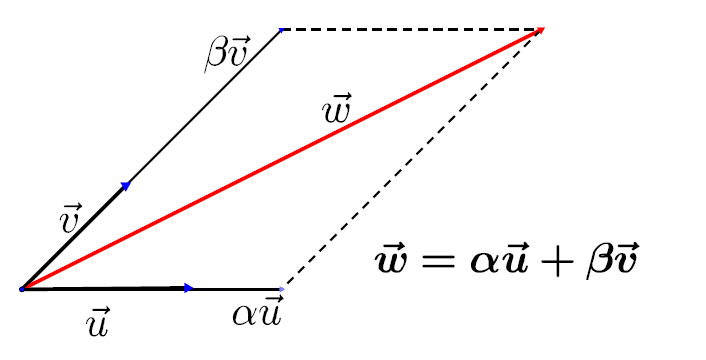
\includegraphics[width=1.0\textwidth]{chapters/combinacao_linear/img/com_linear}
\caption{\footnotesize{ O vetor $\vec{w}$ é uma combinação linear dos vetores $\vec{u}$  e $\vec{v}$}}
\label{fig:comb_linear}
\end{figure}
\end{centering}


\section{Exemplos}
\begin{enumerate}
\item  Considere o espaço vetorial  $\mathbb{P}_2$ dos polinômios de grau menor  ou igual a 2 sobre $\mathbb{R}$. O polinômio $p(x)=5x^2-3x-3$ é uma combinação linear dos polinômios $p_1(x)=x^2-x+1$ e $p_2(x)=-3x^2+x+5$. De fato, verifica-se que $p(x)=2p_1(x)-p_2(x)$.

\item Dados os vetores $v_1=(1,-3,2)$ e $v_2=(2,4,1)$ do espaço vetorial  $\mathbb{R}^3$, temos:
  \begin{enumerate}[label=(\alph*)]
\item O vetor $v=(-4,-18,1)$ é uma combinação linear dos vetores $v_1$ e $v_2$.
\item O vetor $w=(4,3,-6)$  não é uma combinação linear dos vetores $v_1$ e $v_2$.

De fato, no item (a) observe que $$v=2v_1+(-3)v_2.$$  Uma forma de obter os escalares $2$ e $-3$  é  usando a definição de combinação linear, de onde vem a seguinte equação
\begin{align*}(-4,-18,1)&=a_1(1,-3,2)+a_2(2,4,1)\\
                                    &=(a_1+2a_2, -3a_1+4a_2,2a_1+a_2).
\end{align*}

Da iguadade de vetores em $\mathbb{R}^3$, obtemos o sistema linear

\begin{align}
a_1+2a_2&=-4 \nonumber  \\
-3a_1+4a_2 &=-18\nonumber \\
2a_1+a_2&=1. \label{ex2a}
\end{align}
Resolvendo o sistema \eqref{ex2a}, concluimos que $a_1=2$ e $a_2=3$ formam a única solução do mesmo.

Já para o item (b), usamos o mesmo procedimento, obtemos o sistema linear
\begin{align} a_1+2a_2&=4 \nonumber  \\ -3a_1+4a_2 &=3\nonumber \\ 2a_1+a_2&=-6, \label{ex2b}\end{align}   o qual não possui solução. Logo, o vetor $ W$ não é uma combinação linear dos vetores $v_1$ e $v_2$.

\end{enumerate}

\item  O vetor $(3,4)$ do  $\mathbb{R}^2$ pode ser escrito de infinitas maneiras como combinação linear do vetores $(1,0)$, $(0,1)$ e $(2,-1)$. Com efeito, por  definição, o vetor  $(3,4)$ será uma combinação linear dos vetores $(1,0)$, $(0,1)$ e $(2,-1)$ se existirem  escalares $a_1$, $a_2$ e $a_3$ tais que $$(3,4)=a_1(1,0)+ a_2(0,1)+a_3(2,-1).$$ Resolvendo essa equação vetorial, obtemos $$(3,4)=(a_1+2a_3, a_2-a_3),$$  de onde vem   o sistema linear
\begin{align} a_1+2a_3&=3 \nonumber  \\ a_2-a_3&=4. \label{ex3a}\end{align}

Note que o sistema linear \eqref{ex3a} possui mais incógnitas do que equação. Logo  é um sistema indeterminado, ou seja, possui infinitas soluções. Considerando $a_3$ como uma variável livre, a solução geral o sistema linear \eqref{ex3a} é dada por $$\{ ( 3-2a_3, 4+a_3, a_3); a_3 \in \mathbb{R}\}.$$




\end{enumerate}



\section{Subespaços Gerados}

Sejam $V$ um espaço vetorial sobre um corpo  $\mathbb{K}$ e $W=\{v_1, v_2,..., v_n\}$ um subconjunto não vazio de $V$. O conjunto $S$ de \textbf{todas as combinações lineares} dos vetores de $W$ é um subespaço vetorial de $V$.

De fato, $S\neq \emptyset $ pois $$0=0v_1+0v_2+...+0v_n.$$  Isto é, o vetor nulo de $V$ pode ser escrito como uma combinação linear dos vetores de $W$. Agora,  suponha que $w_1$ e $w_2$ são vetores quaisquer de $S$, então existem escalares $a_1, a_2,...,a_n$ e $b_1, b_2,..,b_n$ tais que $$w_1=a_1v_1+ a_2v_2+...+a_nv_n \; \:\text{e} \; \;  w_2=b_1v_1+ b_2v_2+...+b_nv_n.$$ Daí, vem que $$ w_1+w_2=(a_1+b_1)v_1+ (a_2+b_2)v_2+...+(a_n+b_n)v_n .$$ Logo, $w_1+w_2 \in S$ pois também é uma combinação linear de vetores de $W$. Além disso, tem-se que $$\alpha \cdot w_1=(\alpha a_1)v_1+ (\alpha a_2)v_2+...+(\alpha a_n)v_n $$ e, dessa maneira, $\alpha \cdot w_1 \in S$, para todo escalar $\alpha$ e todo $w_1 \in S$. Portanto, $S$ é um subespaço vetorial de $V$.


\vspace{0.3cm}
\textbf{\textit{Observações.}}
  \begin{enumerate}%[label=(\alph*)]
\item Diz-se que $S$ é o  \textit{subespaço  gerado} pelos  vetores  $v_1, v_2,..., v_n$. Ou que $S$ é o  \textit{subespaço  gerado} por $W$. Denota-se $$S=G(W)=[v_1, v_2,..., v_n].$$

\item Os vetores  $v_1, v_2,..., v_n$ são chamados de vetores \textit{geradores}  do subespaço $S$, enquando $W$ é o conjunto \textit{gerador}  do subespaço $S$.

\item Define-se $G(\emptyset)=\{0\}$. Isto é, o espaço gerado pelo conjunto vazio é  o espaço vetorial formado apenas pelo vetor nulo.

\item $W \subset G(W)$. Ou seja, um conjunto de geradores  sempre está contido no subespaço gerado por ele.

\item Todo subconjunto $W $ de um espaço vetorial $V$ gera um subespaço de $V$, podendo $G(W)=V$. Neste caso, diz-se que  $W$ é um gerador de $V$.

\end{enumerate}

\section{Exemplos}

\begin{enumerate}
\item  Em $\mathbb{R}^2$ o vetor  $(1,1)$ gera o subespaço $$U= \{  (x,x); x \in \mathbb{R}\}.$$ Com efeito, qualquer vetor $(x,x) \in U$ pode ser escrito da seguinte maneira $$(x,x)=x\cdot (1,1).$$ Logo, $ U=[(1,1)]$.

\item Os vetores $(1,0)$ e $(0,1)$ geram o espaço $\mathbb{R}^2$. De fato, dado um  vetor $(x,y)$, qualquer, de $\mathbb{R}^2$, têm-se $$(x,y)=x \cdot(1,0)+ y\cdot (0,1).$$ Ou seja, qualquer vetor do $\mathbb{R}^2$ se escreve como uma combinação linear dos vetores $(1,0)$ e $(0,1)$. Portanto, $$[(1,0),(0,1)]=\mathbb{R}^2.$$

\item Um vetor $(x,y)$, qualquer, de $\mathbb{R}^2$, também pode ser escrito do seguinte modo: $$(x,y)=\dfrac{x+y}{2}(1,1)+ \dfrac{y-x}{2}(-1,1).$$ Ou seja, qualquer vetor do $\mathbb{R}^2$ também pode ser escrito como uma combinação linear dos vetores $(1,1)$ e $(-1,1)$. Portanto, $$[(1,1),(-1,1)]=\mathbb{R}^2.$$  \textbf{\textit{Observação.}} Os escalares $\dfrac{x+y}{2}$ e $\dfrac{y-x}{2}$ podem ser calculados resolvendo-se a equação $$(x,y)=a_1(1,1)+a_2(-1,1)$$ em função de $x$ e $y$.



\item O conjunto de polinômios $\{1, t, t^2\}$  gera todo o espaço  $\mathbb{P}_2$. De fato, qualquer polinômio $p(t)$ de grau igual ou menor do que 2 se escreve da seguinte maneira $p(t)=a_2t^2+a_1t+a_0$.

\item Em $\mathbb{M}(2,2)$, temos $\begin{bmatrix}a & b\\0 & c \end{bmatrix} = a\begin{bmatrix} 1 & 0 \\ 0 & 0\end{bmatrix}+b  \begin{bmatrix} 0 & 1\\ 0 & 0\end{bmatrix} + c \begin{bmatrix}0 & 0 \\ 0 & 1 \end{bmatrix}$. Logo, o subespaço das matrizes triângulares superiores de ordem 2 é gerado pelas matrizes $\begin{bmatrix} 1 & 0 \\ 0 & 0\end{bmatrix}$, $\begin{bmatrix} 0 & 1\\ 0 & 0\end{bmatrix}$ e $ \begin{bmatrix}0 & 0 \\ 0 & 1 \end{bmatrix}$.

\item  Se $[u_1,u_2,..,u_k]=U$ e $[w_1,w_2,...,w_k]=W$, então $U+W=[u_1,u_2,..,u_k, w_1,w_2,...,w_k]$. Isto é, se os vetores $u_1,u_2,..,u_k$ geram o subespaço vetorial $U$; e se os vetores $w_1,w_2,...,w_k$ geram o subespaço vetorial $W$, então o subespaço vetorial $U+W$ é gerado pela reunião dos vetores geradores de $U$ com os vetores geradores de $W$.

\end{enumerate}

\section{Dependência e Independência  Linear}

\textbf{Definição.} Sejam $V$ um espaço vetorial sobre um corpo  $\mathbb{K}$ e $v_1, v_2,..., v_n$ vetores de  $V$.  Dizemos que o conjunto $\{v_1, v_2,..., v_n\}$ é um conjunto \textit{linearmente independente (LI)}, ou que os vetores $v_1, v_2,..., v_n$  são $LI$, se a equação $$a_1v_1+a_2v_2+...+a_nv_n=0_v$$ admite apenas a solução nula.  Isto é, se $a_1=a_2=...=a_n=0$.

\vspace{0.3cm}

No caso em que exista algum $a_i \neq 0$ dizemos que o o conjunto $\{v_1, v_2,..., v_n\}$ é um conjunto \textit{linearmente dependente (LD)}, ou que os vetores $v_1, v_2,..., v_n$  são $LD$.

\vspace{0.3cm}

\textit{\textbf{Observação.}} O símbolo $0_v$ na definição acima indica o vetor nulo do espaço vetorial $V$ em questão.

\vspace{0.3cm}
O teorema a seguir estabelece outra caracterização da  depência linear.

\vspace{0.3cm}

 \textit{\textbf{Teorema 1.} O conjunto $\{v_1, v_2,..., v_n\}$ é $ LD$ se, e somente se, pelo menos um desses vetores for combinação linear dos demais.}

\vspace{0.3cm}

\textbf{\textit{Demonstração.}}

Suponha que $\{v_1, v_2,..., v_n\}$ é um conjunto $LD$.  Então, por definição,  a equação

\begin{equation*}
a_1v_1+a_2v_2+...+a_nv_n=0 \label{ld1}
\end{equation*}
admite uma solução diferente da trivial. Isto é, existe uma solução $( a_1, a_2,..., a_n) $ onde pelo menos um $a_i \neq 0$. Vamos supor, sem perda de generalidade, que $a_1 \neq 0$. Assim, obtemos
 \begin{align*}
a_1v_1+a_2v_2+...+a_nv_n&=0 ;\\
a_1v_1&=-a_2v_2-a_3v_3-...-a_nv_n ;\\
v_1&=\dfrac{1}{a_1}(-a_2v_2-...-a_nv_n);\\
v_1&=-\dfrac{a_2}{a_1}v_2-\dfrac{a_3}{a_1}v_3-...-\dfrac{a_n}{a_1}v_n.
\end{align*}
Logo, $v_1$ é uma combinação linear de $\{ v_2,..., v_n\}$.

Por outro lado, suponha que algum dos vetores de $\{v_1, v_2,..., v_n\}$ é uma combinação linear dos demais. sem perda de generalidade, vamos supor que $v_1$ seja esse vetor. Pela definição de combinação linear, existem escalares $( a_2, a_3, ..., a_n) $ tais que
 \begin{align*}
v_1= a_2v_2+a_3v_3+...+a_nv_n.
\end{align*}
Dessa equação, obtemos
 \begin{align*}
v_1-a_2v_2-a_3v_3-...-a_nv_n=0
\end{align*}
que é uma combinação linear nula tendo  o número 1 como o coeficiente de $v_1$. Logo, qualquer solução dessa equação será diferente da solução nula. Portanto, o conjunto de vetores $\{v_1, v_2,..., v_n\}$  é um conjunto $LD$. $\Box$

\vspace{0.3cm}

Equivalentemente ao \textbf{Teorema1} , temos o seguinte:


\vspace{0.3cm}

 \textit{\textbf{Teorema 2.}  O conjunto $\{v_1, v_2,..., v_n\}$ é LI se, e somente se, nenhum desses vetores for combinação linear dos demais.}

\section{Exemplos}
\begin{enumerate}
\item \textit{Em $\mathbb{R}^2$, os vetores $(1,1)$  e $(-1,1)$ são vetores LI. }

 De fato, sejam $a_1$ e $a_2$ tais que  \begin{align*} a_1(1,1) + a_2(-1,1)=(0,0)\\ (a_1-a_2, a_1+a_2)=(0,0).\end{align*} Daí, obtemos o sistema linear
\begin{align*} a_1-a_2&=0   \\ a_1+a_2 &=0\end{align*}    cuja solução é $a_1=a_2=0$.

\item \textit{Em $\mathbb{R}^2$, Os vetores $(1,0)$, $(0,1)$ e $(2,-1)$ são linearmente dependentes. }  De fato, note que o vetor $(2,-1)$ é uma combinação linear dos vetores $(1,0)$ e $(0,1)$  pois $$(2,-1)=2(1,0-1(0,1).$$  Logo pelo  Teorema 1,  o conjunto $\{(1,0), (0,1), (2,-1)\}$ é LD.



\item Sejam  $V$  um espaço vetorial sobre um corpo $\mathbb{K}$ e  vetores $u, v \in V$. Provar que se $u$ e $v$ são LI, então $u + v$ e $ u – v$ também o são.

\textbf{\textit{Demonstração.}} Como queremos mostrar que os vetores $u + v$ e $ u – v$ são LI, considere a combinação linear dando o vetor nulo $ a(u+v)+b(u-v)=0_v$. Devemos mostrar que $a=b=0$.

\begin{align*} a(u+v)+b(u-v)&=0_v   \\
                   au+av+bu-bv &=0_v\\
                   (a+b)u+(a-b)v&=0_v
\end{align*}
Como os vetores $u$ e $v$ são LI, por hipótese, segue da terceira equação que $a$ e $b$ deve satisfazer o sistema de equações
\begin{align*} a+b&=0   \\ a-b &=0,\end{align*} cuja solução é $a=b=0$. $\Box$


\item \textit{ Seja $V$ o espaço vetorial das funções reais contínuas. O conjunto $\{ e^x, e^{-x}\}$, onde $e$ é o número de Euler (base dos logaritmos naturais),  é LI.}

\textbf{\textit{Demonstração.}} Devemos mostrar que a equação $ae^x+ be^{-x}=0$ admite apenas a solução $a=b=0$.  Dada a equação

\begin{equation}
ae^x+ be^{-x}=0, \label{exp1}
\end{equation}
calculemos  a derivada das funções de  ambos os menbros. Daí,  obtemos
\begin{equation}
ae^x- be^{-x}=0.\label{exp2}
\end{equation}

Somando as equações \eqref{exp1} e \eqref{exp2}, vem que

\begin{equation*}
2ae^x=0.
\end{equation*}

Como $2e^x \neq 0$ para todo $x$ real, segue que $a=0$.  Substituindo  o valor de $a$ na equação \eqref{exp1}, obtemos
\begin{equation*}
be^{-x}=0.
\end{equation*}
Como $e^{-x}\neq 0$ para todo $x$ real, segue que $b=0$. Logo, $a=b=0$  e equação $ae^x+ be^{-x}=0$  admite apenas a solução nula. Portanto, o conjunto $\{ e^x, e^{-x}\}$
é LI como queríamos demosntrar. $\Box$
\end{enumerate}

\subsection{Propriedades da Dependência e Independência Linear}

Seja $V$ um espaço vetorial sobre um corpo $\mathbb{K}$.
\begin{enumerate}
\item Se  $W=\{w\}$ e $w \neq 0_v$, então $W$ é LI.
\item Se um conjunto $W \subset V$  contém o vetor nulo, então $W$ é LD.
\item 	Se uma parte do conjunto $W \subset V$  é LD, então $W$  é também LD.
\item 	Se um conjunto  $W$  é LI, qualquer parte $\bar{W}$ de $W$  também é  LI.
\item 	Se $\{v_1, v_2,..., v_n\}$  é LI e  $\{v_1, v_2,..., v_n, w\}$ é LD,então $w$ é combinação linear de  dos vetores  $v_1, v_2,..., v_n$.

\textbf{\textit{Demontração.}} Para provar (i), considere a equação $ \alpha w=0_v$. Como $w\neq 0_v$, então $\alpha=0$ é a única solução possível. Logo pela definição de dependência linear, $W$ é LI.

 Para provar (ii), suponha que  $W$ é um subconjunto de $V$ contendo o vetor nulo. Como podemos escrever o vetor nulo como combinação linear dos demais vetores (basta tomar os coeficientes da combinação linear como sendo o número zero), então pelo Teorema 1, $W$ é um conjunto LD.

Para mostrar que (iii) vale, seja $W=\{v_1, v_2,..., v_k, v_{k+1},...,v_n\}$ um conjunto de $V$ e seja $\bar{W}=\{v_1, v_2,..., v_k\} \subset W$ um conjunto  $LD$. Logo, existe pelo menos um vetor  de $\bar{W}$  que é uma combinação linear dos demais vetores de $\bar{W}$. Digamos que $v_1$ seja esse vetor. Logo,  existem escalares $a_2,...a_k$ tais que $v_1=a_2 v_2+...+ a_kv_k$. Como podemos escrever, $$v_1=a_2 v_2+...+ a_kv_k+0v_{k+1}+...+0v_n,$$
segue $v_1$ também é uma combinação linear dos demais  vetores de $W$ e, portanto, $W$ é um conjunto LD.



Os itens (iv) e (v) fica como exercício.$\Box$


\end{enumerate}


\section{Exercícios Propostos}


\begin{enumerate}

\item 	Sejam os vetores $u = (2,-3,2)$ e $v = (-1,2,4)$ em $\mathbb{R}^3$.
\begin{enumerate}[label=(\alph*)]
\item 	Escrever o vetor $w = (7,-11,2)$ como combinação linear de $u$ e $v$.
\item 	Para que valor de $k$ o vetor $( -8, 14, k)$ é combinação linear de $u$ e $v$?
\item 	Determinar uma condição entre $a$, $b$ e $c$ para que o vetor $(a,b,c)$ seja uma combinação linear de $u$ e $v$.
\end{enumerate}


\item	Consideremos no espaço $\mathbb{P}_2= {at^2 + bt + c; a, b,c \mathbb{R}}$ os vetores $p(t) = t^2 – 2t +1$,
      $q(t) = t + 2$ e $h(t)= 2t^2-t$.
\begin{enumerate}[label=(\alph*)]
\item	Escrever o vetor $m(t) = 5t^2 – 5t + 7$ como combinação linear de $p(t)$, $q(t)$ e $h(t)$.
\item	Escrever o vetor $m(t) = 5t^2 – 5t + 7$ como combinação linear de $p(t)$ e $q(t)$.
\item	Determinar uma condição para $a$, $b$ e $c$ de modo que o vetor $at^2 + bt + c$ seja combinação linear de
      $q(t)$ e $h(t)$.
\item	É possível escrever $p(t)$ como combinação linear de $q(t)$ e $h(t)$?
\end{enumerate}

\item	Considere o subespaço de $\mathbb{R}^4$:
 $$S = [(1,1,-2,4), (1,1,-1,2),(1,4,-4,8)]$$
\begin{enumerate}[label=(\alph*)]
\item	o vetor $(2/3, 1, -1, 2)$ pertence a $S$?
\item	o vetor $(0,0,1,1)$ pertence a $S$?
\end{enumerate}

\item Seja $W$ o subespaço de $\mathbb{M}(2,2)$ definido por $$\left\{ \begin{bmatrix}2a & a+2b \\ 0 & a-b \end{bmatrix}; a,b \in \mathbb{R} \right\}.$$
\begin{enumerate}[label=(\alph*)]
\item $ \begin{bmatrix}0 & -2 \\ 0 & 1 \end{bmatrix} \in W$?
\item  $ \begin{bmatrix}0 & 2 \\ 0 & 1 \end{bmatrix} \in W$?
\end{enumerate}


\item  Seja $W$ o subespaço de $\mathbb{M}(3,2)$  gerado pelas matrizes $\begin{bmatrix}0 & 0 \\ 1& 1 \\0 & 0 \end{bmatrix}$ , $ \begin{bmatrix}0 & 1 \\ 0& -1 \\1& 0 \end{bmatrix}$ e  $\begin{bmatrix}0 & 1\\ 0& 0\\ 0 & 0 \end{bmatrix}$. Verifique se a matriz $\begin{bmatrix}0 & 2\\ 1& 2\\ 3& 0 \end{bmatrix} \in W$.


\item Seja $V=\mathbb{C}[0,1]$ o espaço vetorial das funções reais contínuas no intervalo $[0,1]$. Verifique se cada um dos  subconjutnos a seguir são LI em $V$.

\begin{enumerate}[label=(\alph*)]
\item $\{ x, x+1, x^2-1\} $
\item $\{1, e^x, e^{-x}\}$
\item $\{ senx, cosx\}$.
\end{enumerate}

\item Dados vetores $v_1, v_2,..., v_n$  de um espaço vetorial $V$,  prove que se $w\in V$  é uma combinação linear dos vetores  $v_1, v_2,..., v_n$, então $$[v_1, v_2,..., v_n, w]=[v_1, v_2,..., v_n].$$

\item Sejam $v_1, v_2,..., v_n$ vetores linearmente independentes de um espaço vetorial $V$. Prove que  se $a_1v_1+a_2v_2+...+a_n v_n=b_1v_1+b_2v_2+...+b_n v_n$, então  $a_1=b_1$, $a_2=b_2$,..., $a_n=b_n$.
\item Sejam $V$ um espaço vetorial  e $ u, v, w \in V$. Prove que o conjunto $\{ u, v, w\}$ é LI se, e somente se, o conjunto $\{ u+v, u+w, v+w\} $ é LI.

\item Sejam $V$ um espaço vetorial  e $ u, v, w \in V$. Suponha que $\{ u, v, w\}$ é LI. Dado $t \in V$, existem escalares $\alpha$, $\beta$ e $\gamma$ tais que  $t=\alpha u+\beta v+\gamma w$. Prove que $\{u+t, v+t, w+t\}$ é LI se, e somente se, $\alpha+\beta+\gamma \neq 1$.

\end{enumerate}

%De acordo com a definição anterior, qualquer subespaço de  um espaço vetorial  $V$ deve, necessariamente, conter o vetor nulo de $V$. De fato, a operação de adição de vetores a ser considerada no subconjunto $W$ é  obrigatoriamente a mesma de $V$ e o elemento neutro dessa operação é único.
%
%\vspace{0.3cm}
%Todo espaço vetorial $V$ admite pelo menos dois subespaços: o conjunto formado apenas pelo vetor nulo  e o próprio espaço. Isto é,  $\{ 0\}$ e  $V$. Esses dois subespaços de $V$  são chamados de \textbf{subespaços triviais}.
%
%
%\vspace{0.3cm}
%
%Utilizar a definição de subespaço vetorial para  identificar se um subconjunto $W$  de um espaço vetorial $V$  é um subespaço é  uma atividade laboriosa, pois exige a verificação das oito propriedades,  (A1)-(A4) e (ME1)-(ME4), da definição de espaço vetorial. Felizmente, de acordo com a  próxima proposição,  não precisaremos fazer  a verificação de todas essas propriedades. De fato, sendo  $W$  um subconjunto de $V$,  as propriedades  das operações que são válidas em $V$ devem também ser válidas em $W$, desde que $W$ seja um conjunto fechado em relação a essas operações. Isto é, o resultado das operações realizadas com elementos de $W$  resultam em elementos de $W$.
%
% Um subespaço vetorial $W$ de um espaço vetorial $V$  fica caracterizado pela seguinte proposição:
%
%\textbf{Proposição.} Dados um espaço vetorial $V$ e  um subconjunto $W$ de $V$   não vazio. $W$ é um subespaço de  $V$ se as duas condições a seguir  forem satisfeitas:
%
%\begin{enumerate}[label=(\roman*)]
%\item Se $u$ e $v$ são vetores quaisquer de $W$, então $u+v \in W$;
%\item Se  $ \alpha \in \mathbb{R}$ e $ v$ é um vetor qualquer de $W$, então $\alpha v\in W$.
%
%\end{enumerate}
%
%\textbf{\textit{Observações.}}
%\begin{enumerate}%[label=(\roman*)]
%\item Todo subespaço $W$ de um espaço vetorial $V$ precisa, necessariamente, conter o vetor nulo de $V$. De fato, se tomarmos $\alpha=0$, por (ii),  temos $$0\cdot v=0 $$ para todo $v \in W$.
%
%\item Dessa forma,  se um subconjunto não vazio  $W$ de um espaço vetorial $V$ não possuir o vetor nulo de $V$,  então $W$ não pode ser um subespaço vetorial de $V$.
%\end{enumerate}
%
%\section{Exemplos}
%\begin{enumerate}
%
%
%\item Seja $V=\mathbb{R}^2=\{(x_1, x_2); x_i \in \mathbb{R}\}$ com as operações usuais de  soma de vetores e a multiplicação por escalar.  O subconjunto
%$$W=\{(x, y); y=kx, \; \text{$k$ é uma constante} \}$$ é um subespaço vetorial de $V$.
%
%\textbf{\textit{Demonstração.}}
%Observe que $W$ também pode ser escrito da seguinte maneira:
%$$W=\{(x, kx);  x \in \mathbb{R} \; \text{e}\; \text{$k$ constante} \}.$$   Primeiro é conveniente observar que $(0,0) \in W$. De fato, para $x=0$ teremos $kx=0$, para todo $k\in \mathbb{R}$. Logo, $(0,0) \in W$ e, desse modo, $W \neq \emptyset$.
%
%Agora sejam $u=(x_1, y_1)$ e $v=(x_2, y_2)$ vetores de $W$.  Dessa maneira, podemos escrever $u=(x_1, kx_1)$ e $v=(x_2, kx_2)$. Assim,
%\begin{align*}
%u+v &=(x_1, kx_1)+(x_2, kx_2)\\
%       &=(x_1+x_2, kx_1+kx_2)\\
%       &=(x_1+x_2, k(x_1+x_2)).
%\end{align*}
%Fazendo $x_3=x_1+x_2$, temos que $u+v =(x_3, kx_3)$. Logo, $u+v \in W$ e o item (i) é satisfeito.  Agora seja  $\alpha \in \mathbb{R}$ e $u=(x_1, y_1) \in W$. Assim
%\begin{align*}
%\alpha u &=\alpha(x_1,x_2)\\
%            &=\alpha (x_1, kx_1) \; \text{pois} \;  u \in W;\\
%       &=(\alpha x_1, \alpha k x_1).
%\end{align*}
% Fazendo $x_4=\alpha x_1$ temos que $\alpha u=(x_4, kx_4)$. Logo, $\alpha u \in W$ e o intem (ii) da proposição está satisfeito.  Poranto, $W$ é um subespaço vetorial de $V$. Observe ainda que os elementos de  $W$ descrevem uma reta passando pela origem.
%
%\item Seja $V=\mathbb{R}^2$ e $U=\{(x, 5x+3);  x \in \mathbb{R}\}$.  O subconjunto $U$ não é,  com as operações usuais de  soma de vetores e a multiplicação por escalar, um subespaço vetorial de $\mathbb{R}^2$.   De fato,  o vetor $\{(0,0\}$ não pertence a $W$. Observe que os elementos de $U$ descrevem uma reta em $\mathbb{R}^2$ que não passa pela origem.
%
%
%\item Todos os subespaços de $\mathbb{R}^2$ são:  $\{(0,0)\}$, o  $\mathbb{R}^2$  e os seus subconjuntos que descrevem  retas passando pela origem.
%
%\item Seja $W=\{(x,y,z) \in \mathbb{R}^3; ax+by+cz=0\}$.  Observe que $W$ descreve, em $\mathbb{R}^3$, um \textbf{plano que passa pela origem}.  $W$ é um subespaço vetorial de $\mathbb{R}^3$.
%
%\textbf{\textit{Demonstração.}}
%  Primeiro é conveniente observar que $(0,0,0) \in W$. De fato, para $x=y=z=0$ teremos $ax+by+cz=0$, quaisquer que sejam os escalares  $a,b,c \in \mathbb{R}$. Logo, $(0,0,0) \in W$ e, desse modo, $W \neq \emptyset$.
%
%Agora sejam $u=(x_1, y_1, z_1)$ e $v=(x_2, y_2, z_2)$ vetores de $W$.  Dessa maneira,  temos que $ax_1+bx_1+cz_1=0$ e  $ax_2+bx_2+c_z2=0$. Assim,  temos
%\begin{align*}
%u+v &=(x_1, y_1, z_1)+(x_2, y_2, z_2)\\
%       &=(x_1+x_2, y_1+y_2, z_1+z_2).
%\end{align*}
%Fazendo $x_3=x_1+x_2$,$y_3=y_1+y_2$ e $z_3=z_1+z_2$ temos que
%\begin{align*}
%ax_3+by_3+cz_3&=a(x_1+x_2)+b(y_1+y_2)+c(z_1+z_2)\\
%                             &=\underbrace{ax_1+by_1+cz_1}_{0}+\underbrace{ax_2+by_2+cz_2}_{0}\\
%                             &=0+0=0.
%\end{align*}
%Logo, $u+v  \in W$ e o item (i) é satisfeito.  Agora seja  $\alpha \in \mathbb{R}$ e $u=(x_1, y_1, z_1) \in W$. Assim, $ax_1+bx_1+cz_1=0$.
%\begin{align*}
%\alpha u &=\alpha(x_1,y_1, z_1)\\
%            &=\alpha (x_1,y_1, z_1) \\
%       &=(\alpha x_1, \alpha y_1, \alpha z_1).
%\end{align*}
% Fazendo $x_4=\alpha x_1$, $y_4=\alpha y_1$ e  $z_4=\alpha z_1$ temos que
%\begin{align*}
%ax_4+by_4+cz_4&=a(\alpha x_1)+b(\alpha y_1)+c(\alpha z_1)\\
%                              &=\alpha ( ax_1 +b y_1+cz_1)\\
%                             &=\alpha\underbrace{ax_1+by_1+cz_1}_{0}\\
%                             &=\alpha \cdot 0=0.
%\end{align*}
%Logo, $\alpha u \in W$ e o intem (ii) da proposição está satisfeito.  Portanto, $W$ é um subespaço vetorial de $\mathbb{R}^3$.
%
%
%\item Todos os subespaços de $\mathbb{R}^3$ são:  $\{(0,0,0)\}$, o  $\mathbb{R}^3$, os seus subconjuntos que descrevem  retas passando pela origem e os subconjuntos que descrevem planos passando pela origem.
%
%
%\item Considere em $\mathbb{M}(n,n)$  o conjunto $S$ das matrizes simétricas de ordem $n$.  $S$ é um subespaço vetorial de $\mathbb{M}(n,n)$ . Isto é, $$S=\{ A \in \mathbb{M}(n,n); A^T=A\}.$$ $S$ é um subespaço vetorial de $\mathbb{M}(n,n)$ .
%
%\textbf{\textit{Demonstração.}}
%Primeiro observe que a matriz nula de ordem $n$ é uma matriz simétrica. Logo, $ S \neq \emptyset$.  Agora sejam $A$ e $B$ matrizes simétricas de ordem $n$. Pela propriedade das matrizes  simétricas, temos que $$ (A+B)^T=A^T+B^T. $$
%Por outro lado, $A$ e $B$ são matrizes simétricas. Logo, $A^T=A$ e $B^T=B$. Daí, vem que  $$ (A+B)^T=A^T+B^T = A +B .$$ Ou seja, $A+B$ é uma matriz simétrica. Logo, $A+B \in  \mathbb{M}(n,n)$.
%
%Dado $\alpha \in \mathbb{R}$ e $A$ uma matriz simétrica de ordem $n$, temos, pela propriedade de matriz simétrica, que  $$(\alpha A)^T= \alpha A^T=\alpha A.$$ Assim, $\alpha A$ é uma matriz simétrica, ou seja, $\alpha A \in \mathbb{M}(n,n)$. Portanto, $S$ é um subespaço vetorial de $\mathbb{M}(n,n)$.
%
%
%\item Considere o sistema linear homogêneo $$AX=0$$ onde  $A$, a matriz dos coeficientes, tem  ordem $m \times n$, $X$ é a matriz das incógnitas  e tem ordem $n \times 1$ e $0$ pé matriz dos termos independentes e tem ordem $ m \times 1$.  Seja $S_h$ o conjunto das soluções desse sistema linear homogêo.  Isto é,
%$$S_h=\{ X \in \mathbb{M}(n,1); AX=0 \}.$$  $S_h$ é um subespaço vetorial de $\mathbb{M}(n,n)$ .
%\end{enumerate}
%
%\subsection{Intersecção de Subespaços}
%Seja  $V$ um espaço vetorial sobre um corpo $\mathbb{K}$. Suponha que $U$ e $W$ são  subespaços vetoriais de $V$. Então o conjunto
%$$U\cap W=\{ v \in V;  \; v \in U \; \text{e} \; v \in W \} $$ é um subespaço vetorial de $V$.
%
%\textbf{\textit{Demonstração.}}
%
%Primeiro note que $U\cap W \neq \emptyset$. Isto é, $0 \in U\cap W$. De fato,  como $U$ e $W$ são subespaços de $V$, então $0 \in U$ e $0 \in W$, logo $0 \in U\cap W$.
%
%Agora, vamos mostrar que a soma de dois vetores quaisquer de $U \cap W$ é um vetor de  $U \cap W$.  Para isso suponha que $u,v \in U\cap W$. Dessa forma temos:
%\begin{align*}
%u\in U\cap W&, \; \text{ logo $u \in U$ e $u \in W$};\\
%v\in U\cap W &, \; \text{logo  $v \in U$ e $v \in W$}.
%\end{align*}
%Dessa maneira, temos  $u, v \in U$;   e $u,v \in W$. Como $U$ e $W$ são subespaços, então $u+ v \in U$  e $u+v \in W$. Logo, $$u+ v \in U \cap W. $$
%
%Para mostrarmos que a multiplicação de um vetor de $U\cap W$ por um escalar  também é um vetor $U\cap W$,  considere $\alpha \in \mathbb{K}$  e $u \in U\cap W$.  Desse modo,  $u\in U$ e $u \in W$  (ambos são subespaços de $V$), então   $\alpha \cdot  u \in U$ e $\alpha \cdot  u \in W$.
%Logo, $\alpha \cdot  u\in U\cap W$. Dessa forma concluimos que $U\cap W$ é um subespaço vetorial de $V$.
%
%\subsubsection{Exemplos}
%\begin{enumerate}
%\item Considere os subespaços de $\mathbb{R}^3$
%$$ U= \{(x,y,z) \in \mathbb{R}^3 ; z=0\} $$ e  $$ W= \{(x,y,z) \in \mathbb{R}^3 ; x=0\}.  $$ Seja $(a, b, c)$ um vetor qualquer de $\mathbb{R}^3$. Observe que  $(a, b,c ) \in U\cap W$ se, e somente se,  $(a, b, c) \in U$ e $(a, b, c) \in W$, simultaneamente. Mas, isso somente ocorre se tivermos  $a=0$   e $c=0$. Logo, um  vetor $v$ do $\mathbb{R}^3$ está em $U \cap W$ se, e somente se, $v$ é do tipo $(0, b, 0)$. Assim, escrevemos $$U \cap W=\{(x, y, z) \in\mathbb{R}^3; x=z=0 \}=\{ (0,y,0); y \in \mathbb{R}\}.$$
%
%
%\item Considere em $\mathbb{R}^2$ os subespaços
%$$ U= \{(x,y) \in \mathbb{R}^2 ; y=x\} $$ e  $$ W= \{(x,y) \in \mathbb{R}^2 ; y=-x\}.  $$ Seja $(a, b)$ um vetor qualquer de $\mathbb{R}^2$. Observe que  $(a, b ) \in U\cap W$ se, e somente se,  $(a, b) \in U$ e $(a, b) \in W$, simultaneamente. Mas, isso ocorre somente  se tivermos  $b=a$   e $b=-a$. De onde concluímos que $b=0$ e $a=0$.  Logo, um  vetor $v$ do $\mathbb{R}^2$ está em $U \cap W$ se, e somente se, $v=(0, 0)$. Assim, obtemos $$U \cap W=\{(0,0) \}.$$
%
%\item  Sejam $V= \mathbb{M}(n,n)$ seja o espaço vetorial  das matrizes quadradas, com entradas reais,  de ordem $n$; $U$ o subconjunto  das matrizes triangulares inferiores e $W$ o subconjunto das matrizes triangulares superiores de ordem $n$.  É possível mostrar que $U$ e $W$ são subespaços vetoriais de $V$ (Exercício).  Observe que $U \cap W$ é o conjunto de todas as matrizes diagonais de ordem $n$.
%\end{enumerate}
%
%
%
%\subsection{Soma de Subespaços}
%Seja  $V$ um espaço vetorial sobre um corpo $\mathbb{K}$. Suponha que $U$ e $W$ são  subespaços vetoriais de $V$. Então o conjunto
%$$U+W=\{ v \in V; v=v_1+v_2, \; v_1 \in U \; \text{e} \; v_2 \in W \} $$ é um subespaço vetorial de $V$. O subespaço $U+W$ chama-se \textit{ soma} de $U$ e $W$.
%
%\textbf{\textit{Demonstração.}}
%
%Primeiro note que $U+W \neq \emptyset$. Isto é, $0 \in U+W$. De fato,  como $U$ e $W$ são subespaços de $V$, $0 \in U$ e $0 \in W$. Desse modo, como  $$0=0+0,$$ temos que $0$ pode ser escrito como a soma de um elemento de $U$ com um elemento de $W$.
%
%Sejam $u,v \in U+W$. Dessa forma podemos escrever
%\begin{align*}
%u&=u_1+w_1, \; \text{com $u_1 \in U$ e $w_1 \in W$};\\
%v&=u_2+w_2, \; \text{com $u_2\in U$ e $w_2 \in W$}.
%\end{align*}
%Assim, como $u_1, u_2 \in U$ (e $U$ é um subespaço de $V$), então $u_1+u_2 \in U$.  Do mesmo modo, como $w_1, w_2 \in W$ (e $W$ é um subespaço de $V$), então $w_1+w_2 \in W$.
%
%Desse modo,
%\begin{align*}
%u+v&=(u_1+w_1) + (u_2+w_2) \\
%         &=(u_1+u_2)+(w_1+w_2).
%\end{align*}
%Fazendo $u_3=u_1+u_2$ e $w_3=w_1+w_2$, temos que $u+v=u_3+w_3$, onde $u_3 \in U$ e $w_3 \in W$. Logo, $u+v \in U+W$.
%
%Agora, sejam $\alpha \in \mathbb{K}$  e $u \in U+W$.  Logo, existem $u_1 \in U$ e $w_1 \in W$ tais que $u=u_1+w_1$. Daí,
%\begin{align*}
%\alpha \cdot  u&=\alpha \cdot (u_1+w_1) \\
%         &=\alpha \cdot  u_1+\alpha \cdot  w_1.
%\end{align*}
%Note que $\alpha \cdot  u_1 \in U$ e $\alpha \cdot  w_1 \in W$, pois $U$ e $W$ sao subespaços.  Assim, fazendo $u_4=\alpha \cdot  u_1$ e $w_4=\alpha \cdot  w_1$, temos que $\alpha \cdot  u=u_4+w_4$, onde $u_4 \in U$ e $w_4 \in W$. Logo, $\alpha \cdot  u\in U+W$. Dessa forma concluimos que $U+W$ é um subespaço vetorial de $V$.
%
%\subsubsection{Exemplos}
%\begin{enumerate}
%\item Considere em  $\mathbb{R}^3$, os subespaços
%$$ U= \{(x,y,z) \in \mathbb{R}^3 ; z=0\} $$ e  $$ W= \{(x,y,z) \in \mathbb{R}^3 ; x=y=0\}.  $$ Dado   $(a, b, c)$ um vetor qualquer de $\mathbb{R}^3$, podemos escrever
%$$(a, b, c)= (a,b,0)+(0,0,c).$$
%
% Observe que  $(a, b,0 ) \in U$ e  $(0, 0, c) \in W$. Logo, $(a,b,c) \in U+W$.  Como $(a,b,c)$ é um vetor arbitrário de $\mathbb{R}^3$, concluimos que $$U+W=\mathbb{R}^3.$$
%
%
%\item Considere em $\mathbb{R}^2$, os subespaços
%$$ U= \{(x,y) \in \mathbb{R}^2 ; y=x\} $$ e  $$ W= \{(x,y) \in \mathbb{R}^2 ; y=-x\}.  $$ Seja $(a, b)$ um vetor qualquer de $\mathbb{R}^2$.  Note que  podemos escrever
%$(a, b)$ do seguinte modo: $$(a,b)=\left(\dfrac{a+b}{2},\dfrac{a+b}{2}   \right)+\left(\dfrac{a-b}{2},\dfrac{-a+b}{2}   \right).$$
%
%Como $\left(\dfrac{a+b}{2},\dfrac{a+b}{2}   \right) \in U$ e $\left(\dfrac{a-b}{2},\dfrac{-a+b}{2}   \right) \in W$, então $(a,b) \in U+W$.  Mas, $(a,b)$ é um vetor arbitrário de $\mathbb{R}^2$, logo $$\mathbb{R}^2 = U+W.$$
%
%
%
%\item  Sejam $V= \mathbb{M}(2,2)$ seja o espaço vetorial  das matrizes quadradas, com entradas reais,  de ordem $2$; $U$ o subconjunto  das matrizes triangulares inferiores e $W$ o subconjunto das matrizes triangulares superiores de ordem $2$. Dada  uma matriz  quadrada de ordem 2  qualquer, digamos, $\begin{bmatrix} a & b \\ c & d\end{bmatrix}$, podemos escrever
%$$\begin{bmatrix} a & b \\ c & d\end{bmatrix}= \begin{bmatrix} \frac{a}{2} & 0\\ c & \frac{d}{2}\end{bmatrix}+ \begin{bmatrix} \frac{a}{2} & b \\ 0 & \frac{d}{2}\end{bmatrix}.$$
%Ou seja, qualquer matriz quadrada de ordem 2 pode ser escrita como a soma de um elemento de $U$ (matriz triangular superior) e um elemento de $W$ ( matriz triangular superior). Portanto, $$ U+W=\mathbb{M}(2,2).$$
%
%\end{enumerate}
%
%
%
%
%\subsection{Soma direta}
%
%\textbf{Definição.}  Seja  $V$ um espaço vetorial. Suponha que $U$ e $W$ são  subespaços vetoriais de $V$.  Diz-se que $V$ é a \textit{soma direta } de $U$ e $W$, denota-se $V=U\oplus W$, se
%\begin{enumerate}[label=(\roman*)]
%\item $U \cap W =\{0\}$;
%\item $V=U+W$.
%\end{enumerate}
%
%\subsubsection{Exemplos}
%\begin{enumerate}
%\item No exemplo 1 ( Soma de Subespaços) os subespaços  $$ U= \{(x,y,z) \in \mathbb{R}^3 ; z=0\} $$ e  $$ W= \{(x,y,z) \in \mathbb{R}^3 ; x=y=0\}$$  são tais que  $\mathbb{R}^3=U+W$. Além disso, $U \cap W =\{ (0,0,0) \}$ ( verifique!). Portanto, $$ \mathbb{R}^3 =U\oplus W.$$
%
%\item  No exemplo 2 ( Soma de Subespaços) os subespaços $$ U= \{(x,y) \in \mathbb{R}^2 ; y=x\} $$ e  $$ W= \{(x,y) \in \mathbb{R}^2 ; y=-x\}$$ são tais que
%$\mathbb{R}^2 = U+W$. Além disso, Além disso, $U \cap W =\{ (0,0) \}$ ( verifique!). Portanto, $$ \mathbb{R}^2 =U\oplus W.$$
%
%\item O exemplo 3  (Soma de Subespaços)  temos $ U+W=\mathbb{M}(2,2)$, mas essa soma não pode ser uma soma direta por que $U \cap W $ é formado por todas as matrizes diagonais de ordem 2.
%
%\end{enumerate}
%
%
%
%
%
%
%\section{ Exercícios}
%
%
%\begin{enumerate}
%
%\item  Mostre que $W=\{ ( x, y, z) \in \mathbb{R}^3; z-y=0 \}$ é um  subespaço  vetorial de $\mathbb{R}^3$.
%
%\item Seja $S=\{ (x,y,z) \in \mathbb{R}^3; x+y+z=0\}$  um  plano do $\mathbb{R}^3$  passando pela origem. Mostre que $S$ é um subespaço vetorial  de $\mathbb{R}^3$.
%
%
%\item  Mostre que cada um dos subconjuntos de $\mathbb{R}^4$ a seguir são subespaços vetoriais.
%
%\begin{enumerate}[label=(\alph*)]
%\item $W_1=\{ ( x, y, z, t) \in \mathbb{R}^4; x+y=0 e z-t = 0\}$
%\item $W_2=\{ ( x, y, z, t) \in \mathbb{R}^4; 2x+y-t=0 e z = 0\}$
%\end{enumerate}
%
%\item Verifique se os subconjuntos $U$ e $W$, abaixo, são subespaços vetoriais de $\mathbb{M}(2,2)$.
%\begin{enumerate}[label=(\alph*)]
%\item $U=\left\{ \begin{bmatrix}  a & b\\ c & d \end{bmatrix}; b=c \; \text{e} \; a,b,c,d \in \mathbb{R}\right\}$
%\item $W=\left\{ \begin{bmatrix}  a & b\\ c & d \end{bmatrix}; b=c+1 \; \text{e} \; a,b,c,d \in \mathbb{R}\right\}$
%\end{enumerate}
%
%\item Considere os  subconjuntos de $\mathbb{R}^3$: $U=\{(x, x, x); x \in \mathbb{R} \}$  e $W=\{(x, y, 0); x, y \in \mathbb{R} \}$.
%\begin{enumerate}[label=(\alph*)]
%\item Mostre que $U$ é um subespaço vetorial   de $\mathbb{R}^3$;
%\item Mostre que $W$ é um subespaço vetorial   de $\mathbb{R}^3$;
%\item Mostre que $\mathbb{R}^3= U \oplus W$.
%\end{enumerate}
%
%\item Mostre que o subcojunto das matrizes anti-simétricas de ordem $n$  é um subespaço vetorial de  $\mathbb{M}(n,n)$.
%
%\item Seja $V=\mathbb{F}(\mathbb{R}, \mathbb{R})$ o espaço vetorial  de todas as funções reais e $$P=\{f \in V; f(-x)=f(x), \forall  x \in \mathbb{R} \}. $$ Ou seja, $P$ é o subconjunto das funções pares. Mostre que $P$ é um subespaço vetorial de $V$.
%
%\item Seja $V=\mathbb{F}(\mathbb{R}, \mathbb{R})$ o espaço vetorial  de todas as funções reais.  Verifique se os seguintes subconjuntos de $V$ são subespaços vetoriais.
%\begin{enumerate}[label=(\alph*)]
%\item $W_1 = \{ f \in V; f \; \text{ é contínua}\}$
%\item $W_2 = \{ f \in V; f \; \text{ é derivável}\}$
%\item $W_3 = \{ f \in V; f \; \text{ é integrável}\}$
%\end{enumerate}
%
%item  Sejam $U= \left\{ \left[\begin{array}{cc} a& b\\ c& d\end{array}\right] \in \mathcal{M}(2,2); \; b=c\right\}$ e $W= \left\{ \left[\begin{array}{cc} a& b\\ c& d\end{array}\right] \in \mathcal{M}(2,2); \; a=d=0\; {e} \; b=-c\right\}$.
%    \begin{enumerate}
%    \item Mostre que $U$ e $V$ são subespaços vetoriais de $ \mathcal{M}(2,2)$.
%    \item Mostre que $ \mathcal{M}(2,2)=U \bigoplus V$.
%    \end{enumerate}
%
%
%
%\end{enumerate}

\chapter{Base e Dimensão}
\thispagestyle{empty}


\section{Introdução}

Um espaço vetorial possui, em geral, infinitos vetores. Contudo, já sabemos que alguns espaços vetoriais podem ser gerados a partir de um número finito de seus elementos, através de combinações lineares realizadas com os mesmos. Esse resultado é muito interessante no sentido de que podemos  construir todo um espaço vetorial usando apenas alguns  de seus elementos.  Nessa seção, veremos que conjuntos de geradores que são  linearmente independentes tem essa propriedade. Por exemplo, o conjunto $\{ (1,0), (0,1)\}$  é um conjunto LI de geradores do $\mathbb{R}^2$.  Conjuntos dessa natureza serão chamados de bases e são o tema central da seção.
 \textbf{Atenção.} \textit{Estas notas de aulas tem como objetivo servir de guia  aos alunos que cursam a disciplina álgebra linear, nas turmas sob minha responsabilidade, dos cursos de engenharia da UNIVASF. O uso das mesmas  não dispensa  a leitura  dos livros didáticos indicados nas referências bibliográficas da disciplina, bem como a resolução de exercícios propostos nos mesmos}.

\section{Base}


\textbf{Definição.} Sejam $V$ um espaço vetorial sobre um corpo $\mathbb{K}$ e  $\beta=\{v_1, v_2,..., v_n\}$  um conjunto de vetores não nulos de $V$.  Dizemos que o conjunto $\beta$ é uma base de $V$ se:




\begin{enumerate}[label=(\roman*)]
\item   $\{v_1, v_2,..., v_n\}$ é  LI
\item $\{v_1, v_2,..., v_n\}$  gera $V$. Ou seja, $$ V=[v_1, v_2,..., v_n].$$

\end{enumerate}




\vspace{0.3cm}
De maneira resumida, dizemos que um subconjunto  não-vazio $\beta$ de vetores de um espaço vetorial  $V$  é uma base de $V$ se  $\beta$ é LI e gera $V$.

\vspace{0.3cm}
\textbf{Observações.}
\begin{enumerate}
\item Prova-se que todo espaço vetorial $V\neq \emptyset$ possui uma base. Além disso, se $V$ possui um conjunto gerador com um número finito de elementos diz-se que $V$ é um espaço \textit{finitamente gerado}. Nesse caso, qualquer base de $V$ terá um número finito de elementos.

\item Se $V$ não for um espaço finitamente gerado, então qualquer base de $V$  possui infinitos elementos.  Isso acontece, por exemplo, com o espaço ${F}(\mathbb{X},\mathbb{R})$ das  funções reais definidas em $\mathbb{X} \subset \mathbb{R}$.
\end{enumerate}

\section{Exemplos}

\begin{enumerate}
\item  O subconjunto  $\beta=\{e_1, e_2 \}$  de vetores de $\mathbb{R}^2$,  tal que  $e_1=(1,0)$ e $e_2=(0,1)$,  é uma base do  $\mathbb{R}^2$;

O subconjunto  $\beta=\{e_1, e_2 , e_3\}$  de vetores de $\mathbb{R}^3$, tal que  $e_1=(1,0,0)$, $e_2=(0,1,0)$ e $(0,0,1)$,  é uma base do  $\mathbb{R}^3$. De um modo geral, o conjunto   $$\beta=\{e_1, e_2 ,..., e_n\}$$ é uma base do  $\mathbb{R}^n$.
Tal base é conhecida como \textit{base canônica} do $\mathbb{R}^n$.

\item   Considere o espaço vetorial  $\mathbb{P}_3$ dos polinômios de grau menor  ou igual a 3 sobre $\mathbb{R}$. O subconjunto de $\mathbb{P}_3$ formado pelos  polinômios $$\beta= \{1, t, t^2, t^3\}$$  é uma  base de $\mathbb{P}_3$.  De um modo geral, o conjunto $$\{1, t, t^2,..., t^n\}$$  é uma base do espaço vetorial real $\mathbb{P}_n$. Esta base é chamada de  \textit{base canônica} do $\mathbb{P}_n$.

\item O subconjunto $$\left\{ \begin{bmatrix} 1 & 0 \\ 0 & 0\end{bmatrix}, \begin{bmatrix} 0 & 1\\ 0 & 0\end{bmatrix},\begin{bmatrix}0 & 0 \\ 1 & 0 \end{bmatrix},  \begin{bmatrix}0 & 0 \\ 0 & 1 \end{bmatrix} \right\}$$  é uma base para o espaço vetorial das matrizes quadradas de ordem dois,  $\mathbb{M}(2,2)$. Esta é a base canônica de $\mathbb{M}(2,2)$.

\end{enumerate}


\section{Exercícios resolvidos}

\begin{enumerate}
	\item Mostre que o subconjunto  $\beta=\{(1,1,0), (1,-1,0), (0,0,2)\}$ é uma base do  $\mathbb{R}^3$.



	\item   Mostre que o conjunto $$\beta= \{1, t-1, t^2+t, t^3-t+1\}$$ é uma base  $\mathbb{P}_3$, o espaço dos polinômios de grau menor  ou igual a 3 sobre $\mathbb{R}$.

	\item Mostre que o conjunto $$\left\{ \begin{bmatrix} 1 & 2 \\ 0 & 0\end{bmatrix}, \begin{bmatrix} 1 &0 \\ -1 & 0\end{bmatrix},\begin{bmatrix}0 & 0 \\ 2 & -1 \end{bmatrix},  \begin{bmatrix}0 & 2 \\ 0 & 1 \end{bmatrix} \right\}$$  é uma base para o espaço vetorial das matrizes quadradas de ordem dois,  $\mathbb{M}(2,2)$.

\end{enumerate}













\section{Resultados Importantes}


Dado um conjunto de geradores de um espaço vetorial $V$, sempre podemos extrair  do mesmo uma base de  $V$. Além disso,  se $V$ é um espaço vetorial  gerado por um conjunto finito de $n$ vetores, então quaisquer subconjunto de $V$ com mais de $n$ elementos é, necessariamente,  um conjunto LD.  Essas duas afirmações são apresentadas nos próximos teoremas.
\vspace{0.3cm}

\textit{\textbf{Teorema 1.}  Sejam  $\{v_1, v_2,..., v_n\}$    vetores não nulos que geram um espaço vetorial $V$. Então dentre estes vetores podemos extrair uma base de $V$.}

\vspace{0.3cm}

\textit{\textbf{Teorema 2.} Sejal $V$  um espaço vetorial finitamente gerado pelo  conjunto  de vetores  $\{v_1, v_2,..., v_n\}$.  Então, qualquer conjunto com mais de $n$ vetores é necessariamente LD (e, portanto qualquer conjunto LI tem no máximo n vetores).}

\vspace{0.3cm}

\textit{\textbf{Corolário.} Qualquer base de um espaço vetorial finitamente gerado tem sempre o mesmo número de elementos. }

\vspace{0.3cm}

O fato do número de elementos de uma base de um  espaço vetorial $V$ ser invariante  motiva mais uma definição.: a d\textit{imensão do espaço}. A dimensão de um espaço vetorial, que será definida a seguir, desempenha uma papel importante no estudo dos espaços vetoriais.
\vspace{0.3cm}

\section{Dimensão}
\textbf{Definição.} Seja $V$ um espaço vetorial sobre um corpo $\mathbb{K}$. Se $V$ admite uma base finita, então chamamos de \textit{dimensão de $V$} ao número de elementos de tal base. Caso contrário dizemos que a dimensão de $V$ é infinita.   Denotaremos a dimensão de um espaço  vetorial $V$ por $dim (V)$.


\section{Exemplos}
\begin{enumerate}
\item $dim(\mathbb{R}^n)=n$. Em particular,  $dim(\mathbb{R}^2)=2$  e  $dim(\mathbb{R}^3)=3$.
\item  $dim(\mathbb{P}_n)=n+1$.
\item  $dim(\mathbb{M}(m,n)=m\times n$.
\item  $dim\mathbb ({F}(\mathbb{X},\mathbb{R}))=\infty $.
\end{enumerate}

\textit{\textbf{Teorema 3.} Qualquer conjunto de vetores LI de um espaço vetorial $V$ de dimensão finita pode ser completado de modo a formar uma base de $V$.}

\vspace{0.3cm}

\textit{\textbf{Corolário.} Se $dimV=n$, então  qualquer conjunto de $n$ vetores LI  de $V$ formará uma base de $V$.}

\vspace{0.3cm}

A importância desse corolário está no fato de que se você souber que a dimensão de um espaço vetorial $V$ é 2, por exemplo, e encontrar um conjunto de dois vetores LI, então você pode afirmar que ele  é uma base de $V$.


\section{Coordenadas}

\textit{\textbf{Teorema 4.} Seja $V$ um espaço vetorial sobre um corpo $K$, finitamente gerado e tal que $dim(V) \geq 1$. Então, um conjunto não-vazio $\beta$  de $V$ é uma base de $V$ se, e somente se, cada elemento de $V$ se  escreve de maneira única como uma combinação linear dos vetores de $\beta$.}

\vspace{0.3cm}

O \textit{\textbf{Teorema 4}} estabelece que dada uma base  $\beta=\{v_1, v_2,...,v_n\}$  de $V$, na qual foi  fixada uma ordem nos seus elementos; e dado um vetor $v \in V$, existem escalares $a_1, a_2,..., a_n$ únicos, tais que, $$v=a_1v_1+a_2v_2+...+a_nv_n$$.
Os escalares $a_1, a_2,..., a_n$  são chamados de as \textit{coordenadas} do vetor $v$ em relação à base $\beta$ de $V$. Denotamos $$[v]_{\beta}=\begin{bmatrix} a_1\\ a_2\\ \vdots \\a_n \end{bmatrix}.$$

As coordenadas de um vetor $v \in V$ depende sempre da base $\beta$ escolhida e da ordem de seus elementos.


\section{Exercício Resolvido}
O exercício seguinte estabelece que um espaço vetorial $V$ é uma soma direta dos subespaços gerados por cada um dos vetores que compõem essa base.

\begin{enumerate}
\item \textit{Dado um subconjunto não-vazio $\beta=\{v_1, v_2,..., v_n\}$ de  vetores de um espaço vetorial $V$, mostre que   $\beta$ é uma base de $V$ se, e somente se,  $$V=[v_1]\oplus [v_2]\oplus...\oplus[v_n].$$}

\textit{\textbf{Resolução.}} Suponha que $\beta=\{v_1, v_2,..., v_n\}$ seja uma base de $V$ e sejam $V_1=[v_1], V_2= [v_2], ...,V_n=[v_n]$. Vamos mostrar que $$V_i \cap V_j=\{0\}, \; \text{para todo $i \neq j$};$$  e que $$ V=V_1 +V_2 + ...+ V_n.$$ Primeiro, suponha que $ v \in V_i \cap V_j$. Logo, $v \in V_i$ e $ v \in V_j$. Daí, existem escalares  $a_1$ e $a_2$ tais que  $$ v=a_1v_i \; \; \text{e} \; \; v=a_2v_j.$$ Assim, $$ a_1v_i=a_2v_j.$$  Mas, se $a_1$ e $a_2$ forem, simultaneamente, diferentes de zero, então teríamos
$$ v_i=\dfrac{a_2}{a_1}v_j \; \; \text{e} \; \;  v_j=\dfrac{a_1}{a_2}v_i.$$  Mas, isso não pode ocorrer porque $v_i$ e $v_j$ são vetores LI, já que pertencem a uma base de $V$. Logo, $a_1=0$ e $a_2=0$. Isto é, $v=0$ e assim, $V_i \cap V_j=\{0\}$. Como $V_i$ e $V_j$ foram tomados arbitrariamente, então o resultado vale para para todo $i, j=1,2,...,n$.  Agora seja $v \in V$. Como $\beta=\{v_1, v_2,..., v_n\}$ é uma base de $V$, então existem escalares $a_1, a_2,...,a_n $ tais que $$v=a_1v_1+a_2 v_2+...+a_n v_n.$$  Isso mostra que  $$V=V_1+V_2+...+V_n.$$ Portanto, $$V=V_1\oplus V_2\oplus...\oplus V_n.$$

Por outro lado, suponha que $$V=V_1\oplus V_2\oplus...\oplus V_n.$$ Vamos mostrar que $\beta=\{v_1, v_2,..., v_n\}$  é uma base de $V$. Para isso, precisamos mostrar que $\beta$ gera $V$ e é LI. Como, por hipótese, $V=V_1\oplus V_2\oplus...\oplus V_n$, então $V=V_1+V_2+...+V_n.$ Logo, qualquer vetor $v \in V$ se escreve, do seguinte modo:$$v=a_1v_1+a_2 v_2+...+a_n v_n $$  para alguma sequência de escalares $a_1, a_2,...,a_n $. Como $v$ é arbitrário, segue que $\beta$ gera $V$. Agora, suponha que $\beta=\{v_1, v_2,..., v_n\}$  seja LD. Então existe, $v_j \in \beta$ que é combinação linear dos demais vetores de $\beta$. Digamos, sem perda de generalidade, que $ v_j=av_i$ para algum $i=1,2,..n$ e $i \neq j$. Então, temos que  $av_i \in V_j$ e $ av_i \in V_i$. Logo, $ av_i \in  V_j \cap V_i$. Mas, isso contradiz o fato de que $  V_i \cap V_j = \{0\}$ ( V é soma direta de $V_1, V_2, ..., V_j$).  Portanto, $ \beta$ é um conjunto LI. $\Box$
\end{enumerate}




\section{Exercícios Propostos}


\begin{enumerate}
\item Escreva uma base para o espaço das matrizes de ordem $2\times 3$ com entradas reais. Qual seria uma base para o espaço das matrizes quadradas de ordem $n$?

\item Mostre que o conjunto $\{ 1-t^3, (1-t)^2, 1-t , 1\}$ é uma base de $\mathbb{P}_3$.
\item Dado o subespaço $W$ de $\mathbb{M}(2,2)$ que é gerado pelo conjunto $$\left\{ \begin{bmatrix} 1 & -5 \\ -4 & 2\end{bmatrix}, \begin{bmatrix} 1 & 1\\ -1 & 5\end{bmatrix},\begin{bmatrix}2 & -4 \\ 0 & 7 \end{bmatrix},  \begin{bmatrix}1 & -7 \\-5 & 1 \end{bmatrix} \right\}.$$  Determine uma base de $W$ e a sua dimensão.

\item Considere o subespaço do $\mathbb{R}^4$ gerado pelos vetores $v_1=(1,-1,0,0)$, $v_2=(0,0,1,1)$, $v_3=(-2,2,1,1)$ e $v_4=(1,0,0,0)$.
\begin{enumerate}[label=(\alph*)]
\item 	O vetor $(1, -3,1, 1) \in [v_1, v_2, v_3, v_4]?$
\item Determine uma base de $[v_1, v_2, v_3, v_4]$.
\item  $[v_1, v_2, v_3, v_4]=\mathbb{R}^4$. Por quê?
\end{enumerate}

\item Considere o subespaço do $\mathbb{R}^3$ gerado pelos vetores $v_1=(1,1,0)$, $v_2=(0,-1,1)$ e $v_3=(1,1,1)$.  Verifique se $[v_1, v_2, v_3]=\mathbb{R}^3$.

\item Sejam $U= \{ (x, y, z, t) \} \in \mathbb{R}^4; x+y=0 \; \text{ e } \; z-t=0 $ e $W= \{ (x, y, z, t) \} \in \mathbb{R}^4; 2x+y-t=0 \; \text{ e } \; z=0 $ dois subespaços de $\mathbb{R}^4$.
\begin{enumerate}[label=(\alph*)]
\item 	Determine $ U \cap W$;
\item Determine $ U + W$;
\item Verifique se $\mathbb{R}^4 =U \oplus W$.
\end{enumerate}




\item 	Dados os vetores $u = (2,-1,4,0)$, $v = (1,-2,2,3)$  e $w=(4,-5,8,6)$, faça o que se pede  a seguir.
\begin{enumerate}[label=(\alph*)]
\item Mostre que os vetores $u$, $v$ e $w$ são vetores  LD;
\item Mostre que dois vetores quaisquer constituem uma base para o subespaço $S=[u, v, w]$;
\item Seja o subespaço de $\mathbb{R}^4$  gerado pelos vetores $(0,1,0,0)$ e $(0,0,0,1)$.  Determine o subespaço $ S \cap T$.
\item Quais são as dimensões dos subespaços $S$, $T$, $S \cap T$ e $S+T$?
\item Verifique se  $\mathbb{R}^4 =S \oplus T$.
\end{enumerate}


\item
\begin{enumerate}[label=(\alph*)]
\item Mostre que os conjuntos $\alpha= \{(1,0), (0,1) \}$, $\beta= \{(i,0), (2,-3) \}$ e $\gamma= \{(i,i), (-1,2i) \}$ são bases do espaço vetorial $\mathbb{C}^2$ sobre $\mathbb{C}$.
\item Mostre que o conjunto $\delta= \{(1,0), (i,0), (0,1), (0,i) \}$ é uma  bases do espaço vetorial $\mathbb{C}^2$ sobre $\mathbb{R}$.
\end{enumerate}



\item	Qual é a dimensão do seguinte   subespaço de $\mathbb{R}^4$
 $$S = [(1,1,-2,4), (1,1,-1,2),(1,4,-4,8)]?$$



\item Seja $W$ o subespaço de $\mathbb{M}(2,2)$ definido por $$\left\{ \begin{bmatrix}2a & a+2b \\ 0 & a-b \end{bmatrix}; a,b \in \mathbb{R} \right\}.$$
\begin{enumerate}[label=(\alph*)]
\item Determine uma base de $W$;
\item  Determine $dim(W)$;
\item Determine um subespaço $S$ de $\mathbb{M}(2,2)$ tal que $\mathbb{M}(2,2)= S \oplus W$.
\end{enumerate}


\item  Considere o sistema linear

%\begin{align}
$ (*) \left\{ \begin{array}{rr}
2x+4y-6z&=a\\
x-y+4z&=b \\
6y-14z&=c .
%\end{align}
\end{array}\right.$


Seja $S=\{ (x, y, z) \in\mathbb{R}^3; (x,y,z)\; \text{é solução  de (*)} \}$. Isto é, $S$ é o conjunto-solução do sistema linear (*).
\begin{enumerate}[label=(\alph*)]
\item Que condições devemos impor para $a$, $b$ e $c$ para que o sistema linear seja um subespaço vetorial de  $\mathbb{R}^3$?
\item Nas condições determinadas no ítem (a), determine uma base para $S$.
\item Verifique que  $dim(S)$ é igual ao grau de liberdade do sistema (*).
\end{enumerate}





\end{enumerate}

\chapter{Mudança de Base}
\thispagestyle{empty}

\section{Introdução}

Sejam $V$ um espaço vetorial  e $\beta=\{v_1, v_2,..., v_n \}$ uma base de $V$. Para cada vetor $v \in V$ existem únicos escalares $a_1$, $a_2$,...,$a_n$ tais que

\begin{align*}
v&=a_1v_1+ a_2v_2+ ...+a_nv_n .
\end{align*}

Os escalares $a_1$, $a_2$,...,$a_n$ são chamados de \textit{coordenadas} de $v$ em relação à base $\beta$. Denotamos, $$[v]_{\beta}=\left[ \begin{array}{c}a_1 \\a_2 \\ \vdots \\ a_n\end{array}\right ].$$

\subsection{Exemplos}

\begin{enumerate}
\item Considere $\beta=\{(1,0), (0,1)\}$ a base canônica do $\mathbb{R}^2$ . Observe que o vetor $(2,3) \in \mathbb{R}^2$ pode ser escrito como uma combinar linear dos vetores da base canônica do seguinte modo
\begin{align*}
(2,3)&=2(1,0)+3(0,1).
\end{align*}

Logo, $[(2,3)]_{\beta}=\left[ \begin{array}{c}2 \\3\end{array}\right ].$

De um modo geral, dado um vetor  $(x,y)$ qualquer em $\mathbb{R}^2$, sempre podemos escrever
\begin{align*}
(x,y)&=x(1,0)+y(0,1).
\end{align*}\

Assim as coordenadas de $(x,y)$ em relação à base canônica do $\mathbb{R}^2$ são os próprios escalares $x$ e $y$. Isto é,
$[(x,y)]_{\beta}=\left[ \begin{array}{c}x\\y\end{array}\right ]$. Porém, em relação à outras bases do $\mathbb{R}^2$ as coordenadas de um vetor genérico $(x,y)$ são, em geral, diferentes dos escalares $x$ e $y$.  Por exemplo, considere a base ${\beta} ' = \{ (1,1), (-1,1)\}$  de $\mathbb{R}^2$ . Em relação à esta base o  vetor $(2,3)$ é escrito da seguinte maneira:
\begin{align*}
(2,3)&=\dfrac{5}{2}(1,1)+\dfrac{1}{2}(-1,1).
\end{align*}\
Daí, as coordendas de $(2,3)$ em relação à base ${\beta} '$ são $\dfrac{5}{2}$ e $\dfrac{1}{2}$. Ou seja,$$[(2,3)]_{\beta'}=\left[ \begin{array}{c}\dfrac{5}{2} \\\dfrac{1}{2}\end{array}\right ].$$

\subsection{Observação.} A ordem em que os elementos $v_1, v_2,..., v_n$ de uma base de um espaço vetorial $V$ estão dispostos, nessa base, influi na construção da matriz de coordenadas de um dado vetor $v$, em relação a essa base. Por exemplo, se considerarmos em $\mathbb{R}^2$, as bases $\beta=\{(1,0), (0,1)\}$ e ${\beta}'=\{(0,1), (1,0)\}$, então as coordenadas do vetor $(4,5)$ em relação a essas bases, são dadas por
$[(4,5)]_{\beta}=\left[ \begin{array}{c}4 \\5\end{array}\right ]$ e $[(4,5)]_{\beta '}=\left[ \begin{array}{c}5 \\4\end{array}\right ].$

Por essa razão, deste ponto em diante, dada uma base  $\beta=\{v_1, v_2,..., v_n \}$ de um espaço vetorial  $V$ iremos considerar que a mesma está ordenada na ordem em que seus elementos aparecem.


\end{enumerate}


\section{Mudança de Base}


%\textbf{Definição (Mudança de base).}
Seja  $V$  um espaço vetorial de dimensão finita sobre o conjunto dos números reais. Sejam $\alpha=\{ u_1, u_2, ...,u_n\}$ e $\beta=\{v_1, v_2, ...,v_n\}$ duas bases de $V$. Então existem escalares $x_1, x_2, ...,x_n$ e $y_1, y_2,...,y_n$ tais que
\begin{align}
u&=x_1u_1+ x_2u_2+ ...+x_nu_n
\end{align}\label{eq1}
e
\begin{align}
u&=y_1v_1+ y_2v_2+ ...+y_nv_n.
\end{align}\label{eq2}


Dessa forma, $[u]_{\alpha}=\left[ \begin{array}{c}x_1 \\x_2 \\ \vdots \\ x_n\end{array}\right ]$ e $[u]_{\beta}=\left[ \begin{array}{c}y_1 \\y_2 \\ \vdots \\ y_n\end{array}\right ]$.


Agora, como cada vetor $v_j$, $j=1,2,...,n$, pertence a $V$ e $\alpha$ é uma base de $V$ podemos escrever $v_j$ como combinação linear de dos vetores $u_1, u_2, ...,u_n$ da seguinte maneira:

\begin{align}
v_1&=a_{11}u_1+ a_{21}u_2+ ...+a_{n1}u_n  \nonumber \\
v_2&=a_{12}u_1+ a_{22}u_2+ ...+a_{n2}u_n \nonumber \\
\vdots&=\; \;\;  \; \;\; \; \;\;\; \;\;\; \;\; \vdots \\
v_n&=a_{1n}u_1+ a_{2n}u_2+ ...+a_{nn}u_n \nonumber
\end{align}\label{eq3}

Substituindo a equação (3)  em (2), obtemos

\begin{align}
u&=y_1(a_{11}u_1+ a_{21}u_2+ ...+a_{n1}u_n )+ y_2(a_{12}u_1+ a_{22}u_2+ \nonumber \\
    &+ ...+a_{n2}u_n )+ ...+y_n(a_{1n}u_1+ a_{2n}u_2+ ...+a_{nn}u_n).
\end{align}\label{eq4}

Desenvolvendo os produtos e arrumando a equação  em função de $u_1, u_2,..., u_n$ obtemos:
\begin{align}
u&=(a_{11}y_1+a_{12}y_2+...+a_{1n}y_n)u_1+(a_{21}y_1+a_{22}y_2+...+a_{2n}y_n)u_2+ \nonumber\\
&+...+ (a_{n1}y_1+a_{n2}y_2+...+a_{nn}y_n)u_n.
\end{align}\label{eq5}

Da igualdade entre as equações (1) e (5), devido a unicidade das coordenadas $x_1, x_2, ...,x_n$, obtemos


\begin{align}
x_1&=a_{11}y_1+a_{12}y_2+...+a_{1n}y_n  \nonumber \\
x_2&=a_{21}y_1+a_{22}y_2+...+a_{2n}y_n \nonumber \\
\vdots&=\; \;\;  \; \;\; \; \;\;\; \;\;\; \;\; \vdots \\
x_n&=a_{n1}y_1+a_{n2}y_2+...+a_{nn}y_n. \nonumber
\end{align}\label{eq6}

Usando a notação matricial, obtemos

$$\left[ \begin{array}{c}x_1 \\x_2 \\ \vdots \\ x_n\end{array}\right ]=\left[ \begin{array}{cccc}a_{11}& a_{12} & \hdots & a_{1n}\\a_{21}& a_{22} & \hdots & a_{2n} \\ \vdots & \vdots& \ddots& \vdots\\  a_{n1}& a_{n2} & \hdots & a_{nn}\end{array}\right ] \left[ \begin{array}{c}y_1 \\y_2 \\ \vdots \\ y_n\end{array}\right ].$$


Denotando  $$[I]_{\alpha}^{\beta}=\left[ \begin{array}{cccc}a_{11}& a_{12} & \hdots & a_{1n}\\a_{21}& a_{22} & \hdots & a_{2n} \\ \vdots & \vdots& \ddots& \vdots\\  a_{n1}& a_{n2} & \hdots & a_{nn}\end{array}\right ],$$ obtemos $$[u]_{\alpha}= [I]_{\alpha}^{\beta}[v]_{\beta}.$$


\vspace{1cm}
\textbf{Definição (Mudança de base).} Sejam  $V$  um espaço vetorial de dimensão finita sobre o conjunto dos números reais, $\alpha=\{ u_1, u_2, ...,u_n\}$ e $\beta=\{v_1, v_2, ...,v_n\}$ duas bases de $V$. A matriz $[I]_{\alpha}^{\beta}$ é chamada  a \textit{matriz mudança de base} da base $\beta$ para a base $\alpha$.

\vspace{1cm}
\textbf{Observações}
\begin{enumerate}
 \item A $j-$ésima coluna da  matriz $[I]_{\alpha}^{\beta}$ é  formada pelas coordenadas do vetor $v_j$, da base $\beta$,  em relação à base $\alpha$. Isto é,

$$[I]_{\alpha}^{\beta}=\left[ [v_1]_{\alpha}, [v_2]_{\alpha} ,...,[v_n]_{\alpha}    \right].$$

\item  A matriz $[I]_{\alpha}^{\beta}$  é invertível e a sua inversa é matriz $[I]_{\beta}^{\alpha}$ . Isto é.
$$\left( [I]_{\alpha}^{\beta} \right)^{-1}=[I]_{\beta}^{\alpha}.$$
\end{enumerate}


\subsection{Exemplos}

\begin{enumerate}


\item Considere $\alpha=\{ (1,0), (0,1)\}$ e $\beta=\{(1,1), (-1,1) \}$ duas bases de $\mathbb{R}^2$. Note que
\begin{align*}
(1,1)&=1(1,0)+1(0,1)\\
(-1,1)&=-1(1,0) + 1(0,1).
\end{align*}

Daí, $[(1,1)]_{\alpha}=\left[\begin{array}{c}1\\1 \end{array}\right]$ e $[(-1,1)]_{\alpha}=\left[\begin{array}{c}-1\\1 \end{array}\right]$.

Logo,
$$[I]_{\alpha}^{\beta}=\left[\begin{array}{cc}1&-1\\1&1 \end{array}\right].$$

Por outro lado temos
\begin{align*}
(1,0)&=\dfrac{1}{2}(1,1)-\dfrac{1}{2}(-1,1)\\
(0,1)&=\dfrac{1}{2}(1,1) + \dfrac{1}{2}(-1,1).
\end{align*}

Assim,  $[(1,0)]_{\beta}=\left[\begin{array}{c}\dfrac{1}{2}\\-\dfrac{1}{2} \end{array}\right]$ e $[(0,1)]_{\beta}=\left[\begin{array}{c}\dfrac{1}{2}\\\dfrac{1}{2} \end{array}\right]$.

Logo,
$$[I]_{\beta}^{\alpha}=\left[\begin{array}{cc}\dfrac{1}{2}&\dfrac{1}{2}\\-\dfrac{1}{2}&\dfrac{1}{2}\end{array}\right].$$


Note que $[I]_{\alpha}^{\beta}[I]_{\beta}^{\alpha}=\left[\begin{array}{cc}1&-1\\1&1 \end{array}\right]\left[\begin{array}{cc}\dfrac{1}{2}&\dfrac{1}{2}\\-\dfrac{1}{2}&\dfrac{1}{2}\end{array}\right]=\left[\begin{array}{cc}1&0\\0&1 \end{array}\right].$ Isto é, as matrizes $[I]_{\alpha}^{\beta}$ e $[I]_{\beta}^{\alpha}$ são inversíveis, sendo uma a inversa da outra.


\item Sejam $V$ um espaço vetorial  e $\alpha=\{ u, v, w, t\}$ e $\beta=\{u, u-v, v+w+t, v-t\}$ bases de $V$. Determine $[I]_{\alpha}^{\beta}$ e $[I]_{\beta}^{\alpha}$.

\textit{Resolução.} Para determinarmos $[I]_{\alpha}^{\beta}$ precisamos escrever cada um dos vetores de   ${\beta}$ como combinação linear dos vetores de ${\alpha}$.
Sejam
\begin{align}
v_1&=u  \nonumber\\
v_2&=u-v \\
v_3&=v+w+t \nonumber \\
v_4&=v-t.\nonumber
\end{align}

 Dessa forma,

\begin{align*}
v_1&=1u+0v+0w+0t \\
v_2&=1u+(-1)v+0w+0t \\
v_3&=0u+1v+1w+1t \\
v_4&=0u+1v+0w+(-1)t. \\
\end{align*}

De onde obtemos,

$[v_1]_{\alpha}=\left[ \begin{array}{c} 1\\ 0\\ 0\\ 0\end{array}\right ]$, $[v_2]_{\alpha}=\left[ \begin{array}{c} 1\\ -1\\ 0\\ 0\end{array}\right ]$, $[v_3]_{\alpha}=\left[ \begin{array}{c} 0\\ 1\\ 1\\ 1\end{array}\right ]$ e $[v_4]_{\alpha}=\left[ \begin{array}{c} 0\\ 1\\ 0\\ -1\end{array}\right ]$.

 Logo,

$$[I]_{\alpha}^{\beta}= [v_1]_{\alpha}=\left[ \begin{array}{cccc} 1& 1 &0 &0\\ 0&-1&1&1\\ 0&0&1&0\\ 0&0&1&-1\end{array}\right ].$$


Para obtermos  $[I]_{\beta}^{\alpha}$ precisamos escrever os vetores de $\alpha$ como combinação linear dos vetores de $\beta$. Para isso, basta resolvermos o sistema (6) em função de $v_1$, $v_2$, $v_3$ e $v_4$. Feito isso, obtemos
\begin{align*}
u&=v_1  \nonumber\\
v&=v_1-v_2 \\
w&=-2v_1+2v_2+v_3+v_4 \nonumber \\
t&=v_1-v_2-v_4.\nonumber
\end{align*}

Daí obtemos

$[u]_{\beta}=\left[ \begin{array}{c} 1\\ 0\\ 0\\ 0\end{array}\right ]$, $[v]_{\beta}=\left[ \begin{array}{c} 1\\ -1\\ 0\\ 0\end{array}\right ]$, $[w]_{\beta}=\left[ \begin{array}{c} -2\\ 2\\ 1\\ 1\end{array}\right ]$ e $[t]_{\beta}=\left[ \begin{array}{c} 1\\ -1\\ 0\\ -1\end{array}\right ]$.

 Logo,

$$[I]_{\beta}^{\alpha}= \left[ \begin{array}{cccc} 1& 1 &-2 &1\\ 0&-1&2&-1\\ 0&0&1&0\\ 0&0&1&-1\end{array}\right ].$$

Outra maneira de calcular $[I]_{\beta}^{\alpha}$ é calcular $\left( [I]_{\alpha}^{\beta} \right)^{-1}$.

\end{enumerate}

\section{Exercícios Propostos}
\begin{enumerate}
\item Sejam $\alpha=\{ (1,0), (0,1)\}$, $\beta=\{ (-1,1), (1,1)\}$  e $\gamma=\{ (\sqrt{3},1), ((\sqrt{3},-1)\}$.
\begin{enumerate}[label=(\alph*)]
\item Determine a matriz mudança de base da base $\beta$ para a base $\alpha$, $[I]_{\alpha}^{\beta}$.
\item Determine a matriz mudança de base da base $\alpha$ para a base $\beta$, $[I]_{\beta}^{\alpha}$.
\item Determine  $[I]_{\gamma}^{\alpha}$ e $[I]_{\alpha}^{\gamma}$.
\item Calcule as coordenadas de $v=(3,-2)$ em relação a cada uma das bases $\alpha$, $\beta$ e $\gamma$.
\end{enumerate}
\item Dadas duas bases $\alpha$ e $\beta$ de $\mathbb{R}^3$ tais que  $[I]_{\alpha}^{\beta}=\left[ \begin{array}{ccc} 1& 1 &0\\ 0&-1&1\\ 1&0&-1\end{array}\right ]$.
\begin{enumerate}[label=(\alph*)]
\item Calcule $[v]_{\alpha}$ sabendo-se que  $[v]_{\beta}=\left[ \begin{array}{c} -1\\ 2\\ 3\end{array}\right ]$.
\item Calcule $[v]_{\beta}$ sabendo-se que  $[v]_{\alpha}=\left[ \begin{array}{c} -1\\ 1\\ 2\end{array}\right ]$.
\end{enumerate}

\item Seja  $\alpha$ a base canônica do $\mathbb{R}^2$ e  seja $\beta$ a base obtida da base $\alpha$ pela rotação de um ângulo $-\dfrac{\pi}{3}$. Ache $[I]_{\alpha}^{\beta}$ e $[I]_{\beta}^{\alpha}$.

\item Seja $\alpha = \{ v_1, v_2, ..., v_n\}$ uma base de um espaço vetorial $V$. Mostre  que  $[I]_{\alpha}^{\alpha}= I_n$, onde $I_n$ é a matriz identidade de ordem $n$.


\end{enumerate}

\chapter{A Matriz de uma Transformação  Linear}
\thispagestyle{empty}

\section{Introdução}
O objetivo deste tópico é  possibilitar o trabalho com  transformações lineares através do estudo de  matrizes associadas a essas transformações. A abordagem do estudo de tranformações lineares via matrizes é interessante por que, de um modo geral, os problemas fundamentais da álgebra linear, a resolução de sistemas lineares e cálculo de autovalores e autovetores, se reduzem ao  trabalho com matrizes.


Inicialmente note que dada uma matriz $A$ de ordem $m\times n$ podemos definir uma aplicação $T_A: \mathbb{R}^n \rightarrow \mathbb{R}^m$ por
\begin{align}
T_A(x)=Ax \label{matrizTa}
\end{align}
para todo $x=(x_1, x_2, ..., x_n) \in \mathbb{R}^n$. Para tornar compatível as operações matriciaiso o vetor $x$ é tomado como a matriz coluna $x=\left[ \begin{array}{c}x_1 \\ x_2 \\ \vdots \\ x_n\end{array} \right]$.

%\textbf{Proposição.}
 A aplicação $T_A$ definida em \eqref{matrizTa} é uma transformação  linear.  De fato, sejam  $x$ e $y$  vetores pertencentes ao $\mathbb{R}^n$ e  $\alpha$ um escalar. Usando a definição de $T_A$ e as  propriedades das operações matriciais,  temos $$T_A(x+\alpha y)=A(x+\alpha y)=Ax+\alpha Ay=T_A(x)+\alpha T_A(y).$$
Ou seja, $T_A$ é linear.  Dessa forma, a cada matriz $A$ de ordem $m\times n$ podemos associar uma transformação linear  $T_A: \mathbb{R}^n \rightarrow \mathbb{R}^m$. A recíproca dessa afirmação também é verdadeira. Isto é, a cada transformação linear $T: \mathbb{R}^n \rightarrow \mathbb{R}^m$ podemos associar uma matriz $A$ de ordem $m\times n$.


A seguir veremos  que esse resultado pode ser  generalizado  para transformações  lineares quaisquer, entre espaços vetoriais de dimensão finita quaisquer. Também veremos  um  procedimento para obter  a matriz de uma transformação linear qualquer.

\section{A Matriz de uma Transformação Linear}


Sejam $U$ e $V$ espaços vetoriais sobre $\mathbb{R}$,  $T: U \rightarrow V$ uma transformação linear, $\alpha=\{ u_1, u_2, ...,u_n\}$ uma base $U$ e $\beta=\{v_1, v_2, ...,v_m\}$ uma base de $V$.  Dessa forma, dado $u\in U$, existem  únicos escalares $a_1$, $a_2$,...,$a_n$ tais que

\begin{align}
u&=a_1u_1+ a_2u_2+ ...+a_nu_n .
\end{align}

Como $T$ é linear, então obtemos

\begin{align}
T(u)&=a_1T(u_1)+ a_2T(u_2)+ ...+a_nT(u_n).
\end{align}

%Além disso, como $T(u) \in V$ existem  únicos escalares $b_1$, $b_2$,...,$b_n$ tais que
%
%\begin{align}
%T(u)&=b_1v_1+ b_2v_2+ ...+b_mv_m .
%\end{align}

Mais adiante voltaremos as equações (1) e (2). Por enquanto, observe que como $T(u_1)$,  $T(u_2)$,...,$T(u_n)$ são vetores de $V$,  então existem escalares $a_{ij}$, com $1\leq i \leq m$  e $1\leq j \leq n$ tais que

\begin{align}
T(u_1)&=a_{11}v_1+ a_{21}v_2+ ...+a_{m1}v_m \nonumber \\
T(u_2)&=a_{12}v_1+ a_{22}v_2+ ...+a_{m2}v_m \nonumber \\
      \vdots&= \vdots \\
T(u_n)&=a_{1n}v_1+ a_{2n}v_2+ ...+a_{mn}v_m \nonumber
\end{align}

Daí obtemos a matriz de coordenadas (ou vetor de coordenadas, já que possui uma única coluna), em relação a base $\beta$, de $T(u_1)$, $T(u_2)$,..., $T(u_n)$. Isto é,

$[T(u_1)]_{\beta}=\left[ \begin{array}{c}a_{11} \\ a_{21} \\ \vdots \\ a_{m1}\end{array} \right]$, $[T(u_2)]_{\beta}=\left[ \begin{array}{c}a_{12} \\ a_{22} \\ \vdots \\ a_{m2}\end{array} \right]$, ..., $[T(u_n)]_{\beta}=\left[ \begin{array}{c}a_{1n} \\ a_{2n} \\ \vdots \\ a_{mn}\end{array} \right]$.


\vspace{1cm}

\textbf{Definição (Matriz de uma tranformação linear).}  A matriz da transformação linear $T: U \rightarrow V$ em relação às bases $\alpha$ e $\beta$, denotamos $[T]_{\beta}^{\alpha}$, é a matriz cujas colunas são formadas pelos elementos das matrizes de coordenadas $ [T(u_1)]_{\beta},  [T(u_2)]_{\beta},..., [T(u_n)]_{\beta}$. Isto é,
\vspace{0.3cm}
$$[T]_{\beta}^{\alpha}=\left[ \begin{array}{cccc}a_{11} &a_{21} & \hdots & a_{1n} \\ a_{21} & a_{22} & \hdots & a_{2n} \\ \vdots & \vdots & \ddots & \vdots \\ a_{m1}& a_{m_2} & \hdots & a_{mn} \end{array} \right].$$


\subsection{Exemplos}

\begin{enumerate}
\item
Sejam $\alpha=\{ (1,1), (-1,1)\}$ uma base $\mathbb{R}^2$,  $\beta=\{(1,1,1), (1,1,0),(1,0,0)\}$ uma  base de $\mathbb{R}^3$  e $T: \mathbb{R}^2 \rightarrow \mathbb{R}^3$ e  a transformação linear definida por $T(x,y,z)=(x,x+y,y)$. Determine a matriz  de $T$ em relação as bases ${\alpha}$ e ${\beta}$. Isto é, $[T]_{\beta}^{\alpha}$.

\vspace{0.5cm}
\noindent\textit{Resolução.} Por definição,  $[T]_{\beta}^{\alpha}$ é  a matriz cujas colunas são formadas pelos vetores  $[T(1,1)]_{\beta}$  e  $[T(-1,1)]_{\beta}$, nessa ordem. Logo, precisamos calcular primeiro $T(1,1)$ e $T(-1,1)$ e em seguida as suas coordendas em relação a base $\beta$.

\vspace{0.5cm}
\textbf{1. Cálculo de  $T(1,1)$ e de suas coordenadas na base $\beta$, $[T(1,1)]_{\beta}$.}

Como $T(1,1)=(1, 2, 1)$, devemos calcular $a_{1}$, $a_{2}$ e $a_{3}$, tais que,

\begin{align*}
(1,2,1)&=a_1(1, 1, 1)+a_2(1,1,0)+a_3(1,0,0), \\
(1,2,1)&=(a_1+a_2+a_3, a_1+a_2,a_1).
\end{align*}
Daí  obtemos o sistema linear
\begin{align*}
a_1+a_2+a_3 &=1 \\
a_1+a_2 &=2 \\
a_1&= 1,
\end{align*}
cuja solução é $a_1=-1$, $a_2=1$ e $a_3=-1$. De onde obtemos
$[T(1,1)]_{\beta}=\left[ \begin{array}{c}-1 \\ 1 \\ -1\end{array} \right]$.

\vspace{0.5cm}
\textbf{2. Cálculo de  $T(-1,1)$ e de suas coordenadas na base $\beta$, $[T(-1,1)]_{\beta}$.}

Como $T(-1,1)=(-1, 0, 1)$, devemos calcular $a_{1}$, $a_{2}$ e $a_{3}$, tais que,

\begin{align*}
(-1,0,1)&=a_1(1, 1, 1)+a_2(1,1,0)+a_3(1,0,0), \\
(-1,0,1)&=(a_1+a_2+a_3, a_1+a_2,a_1).
\end{align*}

Analogamente, ao primeiro caso, resolvemos  o sistema linear
\begin{align*}
a_1+a_2+a_3 &=-1 \\
a_1+a_2 &=0 \\
a_1&= 1,
\end{align*}
cuja solução é $a_1=0$, $a_2=0$ e $a_3=-1$ e  obtemos
$[T(-1,1)]_{\beta}=\left[ \begin{array}{c}0 \\0\\ -1\end{array} \right]$.

\textbf{3. Escrevemos a matriz de $T$.}

Finalmente, temos a matriz $$[T]_{\beta}^{\alpha}=\left[ \begin{array}{cc}-1 &0 \\ \;\;1 &0  \\  -1& -1 \end{array} \right].$$

%$$[T]_{\beta}^{\alpha}=\left[ \begin{array}{cc}a_{11} &a_{12} \\ a_{21} & a_{22}  \\  a_{31}& a_{32} \end{array} \right].$$

\item Dado  $\alpha =\{e_1, e_2, e_3, e_4\}$ a base canônica do $ \mathbb{R}^4 $ e $\beta=\{(1,1,1), (0,1,1),(0,0,1)\}$ uma base do $ \mathbb{R}^3$, determinar a transformação linear  $T: \mathbb{R}^4 \rightarrow \mathbb{R}^3$  tal que
$$[T]_{\beta}^{\alpha}=\left[ \begin{array}{cccc}1 &2&3&0 \\ -1 &0&1&1  \\  5&4&0&-2 \end{array} \right].$$

\vspace{0.5cm}
\noindent\textit{Resolução.}  Primeiro note que pela definição de  $[T]_{\beta}^{\alpha}$ , temos:

$[T(e_1)]_{\beta}=\left[ \begin{array}{c}1 \\-1\\ 5\end{array} \right]$, $[T(e_2)]_{\beta}=\left[ \begin{array}{c}2 \\0\\ 4\end{array} \right]$,$[T(e_3)]_{\beta}=\left[ \begin{array}{c}3\\1\\ 0\end{array} \right]$ e $[T(e_4)]_{\beta}=\left[ \begin{array}{c}0 \\1\\ -2\end{array} \right]$.
Dessa maneira, obtemos:
\begin{align*}
T(e_1)&=1(1, 1, 1)+(-1)(0,1,1)+5(0,0,1)=(1,0,6), \\
T(e_2)&=2(1, 1, 1)+0(0,1,1)+4(0,0,1)=(2,2,6), \\
T(e_3)&=3(1, 1, 1)+1(0,1,1)+0(0,0,1)=(3,4,4), \\
T(e_4)&=0(1, 1, 1)+1(0,1,1)+(-2)(0,0,1)=(0,1,-1).
\end{align*}

Agora o problema se reduz a encontrar uma transformação linear $T: \mathbb{R}^4 \rightarrow \mathbb{R}^3$ tal que
 \begin{align*}
T(e_1)&=(1,0,6), \\
T(e_2)&=(2,2,6), \\
T(e_3)&=(3,4,4), \\
T(e_4)&=(0,1,-1).
\end{align*}
Para isto, consideremos um vetor genérico do $ \mathbb{R}^4$, isto é, $(x,y,z,w)$ e vamos escrevê-lo como combinação linear dos vetores da base $\alpha =\{e_1, e_2, e_3, e_4\}$. Ou seja, $$(x,y,z,w)= xe_1+ y e_2+z e_3+ we_4.$$
Como $T$ é linear, obtemos:
\begin{align*}
T(x,y,z,w)&= xT(e_1)+ y T(e_2)+z T(e_3)+ wT(e_4),\\
                &= x(1,0,6)+ y (2,2,6)+z (3,4,4)+ w(0,1,-1),\\
               &=(x+2y+3z, 2y+4z+w,6x+6y+4z+w).
\end{align*}

Portanto, a transformação linear procurada é  $$T(x,y,z,w)=(x+2y+3z, 2y+4z+w,6x+6y+4z+w).$$


\item \textbf{Matriz da transformação Identidade e a matriz mudança de base.} Sejam $\alpha =\{u_1, u_2, ..., u_n\}$ e $\beta =\{v_1, v_2, ..., v_n\}$ duas bases distintas de $U$   e  $T:U \rightarrow U$ a transformação linear  identidade, isto é,   $T(u)=u$ para todo $u\in U$. Então a matriz de $T$ em relação às bases  $\alpha$ e  $\beta$ é igual a matriz de mudança de base, da base $\alpha$ para a base  $\beta$. Ou seja,  $[T]_{\beta}^{\alpha}$ = $[I]_{\beta}^{\alpha}$.

\noindent\textit{Demonstração.}  Neste caso, observe que como $T(u_i)=u_i$ para $i=1,2,..,n$, então quando calculamos as coordenadas de  $T(u_1), T(u_2),..., T(u_n)$ na base $\beta =\{v_1, v_2, ..., v_n\}$, estamos,  na verdade, calculando as coordenadas de  $u_1, u_2,..., u_n $ na base $\beta =\{v_1, v_2, ..., v_n\}$. Ou seja,
\begin{align*}
T(u_1)&=u_1=a_{11}v_1+ a_{21}v_2+ ...+a_{n1}v_n \\
T(u_2)&=u_2=a_{12}v_1+ a_{22}v_2+ ...+a_{n2}v_n  \\
      \vdots&= \vdots \\
T(u_n)&=u_n=a_{1n}v_1+ a_{2n}v_2+ ...+a_{nn}v_n
\end{align*}

Assim,  obtemos $$[T]_{\beta}^{\alpha}=\left[ \begin{array}{cccc}a_{11} &a_{21} & \hdots & a_{1n} \\ a_{21} & a_{22} & \hdots & a_{2n} \\ \vdots & \vdots & \ddots & \vdots \\ a_{n1}& a_{n_2} & \hdots & a_{nn} \end{array} \right]=[I]_{\beta}^{\alpha}.$$

\vspace{0.5cm}
\item Quando temos transformações lineares  $T: \mathbb{R}^{m} \rightarrow \mathbb{R}^{n}$  e as bases $\alpha$ e $\beta$  consideradas são as bases canônicas dos espaços envolvidos, então é comum representarmos a matriz da transformação $T$, simplesmente, por $[T]$. Por exemplo, considere  a transformação linear $T: \mathbb{R}^{3} \rightarrow \mathbb{R}^{2}$ definida por $T(x,y,z)= (z-x, z-y)$. A matriz de $T$ em relação as bases canônicas  $\alpha =\{ e_1, e_2, e_3\}$ e  $\beta =\{ e_1, e_2\}$ do $\mathbb{R}^{3}$ e  $\mathbb{R}^{2}$, respectivamente, é a  matriz
 $$[T]=\left[ \begin{array}{ccc} -1 & 0 & 1 \\ 0 & -1 & 1 \end{array} \right].$$

\item Sejam $T: \mathcal{P}_2(\mathbb{R}) \rightarrow \mathbb{R}^{3}$  definida por $$T(a_0+a_1t+a_2t^2)=(a_0,a_1,a_2),$$ $\alpha = \{ 1, t, t^2\}$ base de  $\mathcal{P}_2(\mathbb{R})$ e $\beta =\{ (1,0,1), (0,1,1), (1,1,0)\}$   base de $\mathbb{R}^{3}$. Determinar $[T]_{\beta}^{\alpha}$.


\noindent\textit{Resolução.} Primeiro note que $1= 1+0\cdot t+0\cdot t^2$, $t=0\cdot 1+1\cdot t+0 \cdot t^2$ e $t^2=0\cdot 1+0\cdot t+1\cdot t^2$. Dessa maneira,

\begin{align*}
T(1)&=T(1 \cdot 1+0\cdot t+0\cdot t^2)=(1,0,0)\\
T(t)&=T(0\cdot 1+1\cdot t+0 \cdot t^2)=(0,1,0)\\
 T(t^2)&=T(0\cdot 1+0\cdot t+1\cdot t^2)=(0,0,1).
\end{align*}

Para calcular as coordenas desses vetores na base $\beta$ do $\mathbb{R}^{3}$ precisamos resolver os  sistemas lineares  dados pelas seguintes equações:

\begin{align*}
(1,0,0)&=a_{11}(1,0,1) + a_{21} (0,1,1)+a_{31}(0,1,1) \\
(0,1,0)&=a_{12}(1,0,1) + a_{22} (0,1,1)+a_{32}(0,1,1) \\
(0,0,1)&=a_{13}(1,0,1) + a_{23} (0,1,1)+a_{33}(0,1,1) \\
\end{align*}

 De onde, obtemos
$$[T]_{\beta}^{\alpha}=\left[ \begin{array}{ccc}1/2 &-1/2&1/2 \\ -1/2 &1/2&1/2  \\  1/2&1/2&-1/2 \end{array} \right].$$


\end{enumerate}

\section{Exercícios Propostos}
\begin{enumerate}
\item Determine  a matriz da tranformação  em relação à base canônica  da transformação linear $T: \mathbb{R}^3 \rightarrow \mathbb{R}^3$ definida por $T(x,y, z)=(z-x,z-y,z)$.


\item  Seja $T: \mathbb{R}^2 \rightarrow \mathbb{R}^2$ definida por $T(x,y)=(xcos\theta - ysen\theta,xsen\theta+ ycos\theta)$. Determine $[T]_{\beta}^{\alpha}$ sendo $\alpha =\{(1,1), (-1, 1) \}$ e $\beta =\{ e_1, e_2\}$.

\item Determine  a matriz de cada das seguintes tranformações  lineares $T: \mathbb{R}^2 \rightarrow \mathbb{R}^2$,  em relação à base canônica  $\mathbb{R}^2$.
\begin{enumerate}
\item  $T(x,y)=c(x,y)$ para todo $c \in \mathbb{R}$ (\textit{Contração ou expansão}).
\item  $T(x,y)=(x,-y)$  (\textit{Reflexão em torno do eixo x}).
\item $T(x,y)=(-x,-y)$  (\textit{Reflexão na origem}).
\item  $T(x,y)=(x+cy,y)$ para todo $c \in \mathbb{R}$ (\textit{Cisalhamento horizontal}).
\end{enumerate}
\end{enumerate}

\noindent\textbf{Teorema 1.} Sejam $U$ e $V$ espaços vetoriais, $\alpha$ e $\beta$ bases de $U$ e de $V$, respectivamente, e $T: U \rightarrow V$ uma transformação linear. Então, para cada $u\in U$ vale $$ [T(u)]_{\beta}=[T]_{\beta}^{\alpha}[u]_{\alpha}.$$

\begin{figure}[h]
\center
% \includegraphics[width=1.0\textwidth]{matriztransf}
\caption{\footnotesize{As coordenadas de $T(u)$ na base $\beta$ é igual ao produto da matriz de $[T]_{\beta}^{\alpha}$ pelo vetor das coordendas de $u$ na base $\alpha$.}}
\label{fig:exp}
\end{figure}



\noindent\textit{\textbf{Demonstração.}} Considerando que  $\alpha =\{u_1, u_2, ..., u_n\}$ e $\beta =\{v_1, v_2, ..., v_n\}$ são as bases de $U$ e $V$, respectivamente. Basta voltarmos às equações (1), (2) e (3) do início do texto.  Substituindo as equações de (3) na equação (2), obtemos:
\begin{align}
T(u)&=a_1(a_{11}v_1+ a_{21}v_2+ ...+a_{m1}v_m)+ a_2(a_{12}v_1+ a_{22}v_2+ ...+a_{m2}v_m )+ \nonumber\\
       & + ...+a_n(a_{1n}v_1+ a_{2n}v_2+ ...+a_{mn}v_m).
\end{align}

A equação  (4) pode ser reescrita da seguinte maneira:
\begin{align}
T(u)&=(a_1a_{11}+a_2a_{12}+...+a_na_{1n})v_1+(a_1a_{21}+a_2a_{22}+...+a_na_{2n})v_2+ \nonumber\\
     &=+...+(a_1a_{m1}+a_2a_{m2}+...+a_na_{mn})v_m.
\end{align}

Daí, fazendo
\begin{align}
b_1&=a_1a_{11}+a_2a_{12}+...+a_na_{1n} \nonumber\\
b_2&=a_1a_{21}+a_2a_{22}+...+a_na_{2n} \nonumber\\
 \vdots& = \vdots \nonumber\\
b_m&=a_1a_{m1}+a_2a_{m2}+...+a_na_{mn}
\end{align}

Obtemos, na forma matricial,
$$\left[ \begin{array}{c} b_1\\ b_2 \\ \vdots \\ b_m \end{array} \right]=\left[ \begin{array}{cccc}a_{11} &a_{21} & \hdots & a_{1n} \\ a_{21} & a_{22} & \hdots & a_{2n} \\ \vdots & \vdots & \ddots & \vdots \\ a_{m1}& a_{m_2} & \hdots & a_{mn} \end{array} \right]\left[ \begin{array}{c} a_1\\ a_2 \\ \vdots \\ a_n \end{array} \right].$$

Mas, note de (1), (3) e de (5) que $\left[ \begin{array}{c} a_1\\ a_2 \\ \vdots \\ a_n \end{array} \right]=[u]_{\alpha}$, $\left[ \begin{array}{cccc}a_{11} &a_{21} & \hdots & a_{1n} \\ a_{21} & a_{22} & \hdots & a_{2n} \\ \vdots & \vdots & \ddots & \vdots \\ a_{m1}& a_{m_2} & \hdots & a_{mn} \end{array} \right]=[T]_{\beta}^{\alpha}$ e que  $\left[ \begin{array}{c} b_1\\ b_2 \\ \vdots \\ b_m \end{array} \right]=[T(u)]_{\beta}$. Portanto, temos $$ [T(u)]_{\beta}=[T]_{\beta}^{\alpha}[u]_{\alpha}.$$


\section{Matriz da composição de tranformações lineares}

O próximo teorema  estabelece que a matriz de uma composição de transformações lineares é igual ao produto das matrizes das transformações envolvidas em relação as bases consideradas para os seus  respectivos domínios e contradomínios.  Essa é uma das vantagens de se trabalhar com as matrizes de transformações lineares,  pois o cálculo de  produto de matrizes pode ser efetuado eficientemente através de computadores. A \textbf{Figura 2} ilustra a composição de duas transformações lineares $T_1$ e $T_2$ do teorema abaixo.

\vspace{0.5cm}

\noindent\textbf{Teorema 2.} Sejam  $T_1: U \rightarrow V$  e $T_2: V \rightarrow W$ transformações lineares e $\alpha$,  $\beta$ e $\gamma$ bases de $U$, $V$ e $W$  respectivamente. Então a aplicação composta de $T_1$ com $T_2$, $$T_2 \circ T_1: U \rightarrow W,$$  é uma transformação linear e $$[T_2 \circ T_1]_{\gamma}^{\alpha}=[T_2 ]_{\gamma}^{\beta} \cdot[T_1]_{\beta}^{\alpha}.$$

\begin{figure}[h]
\center
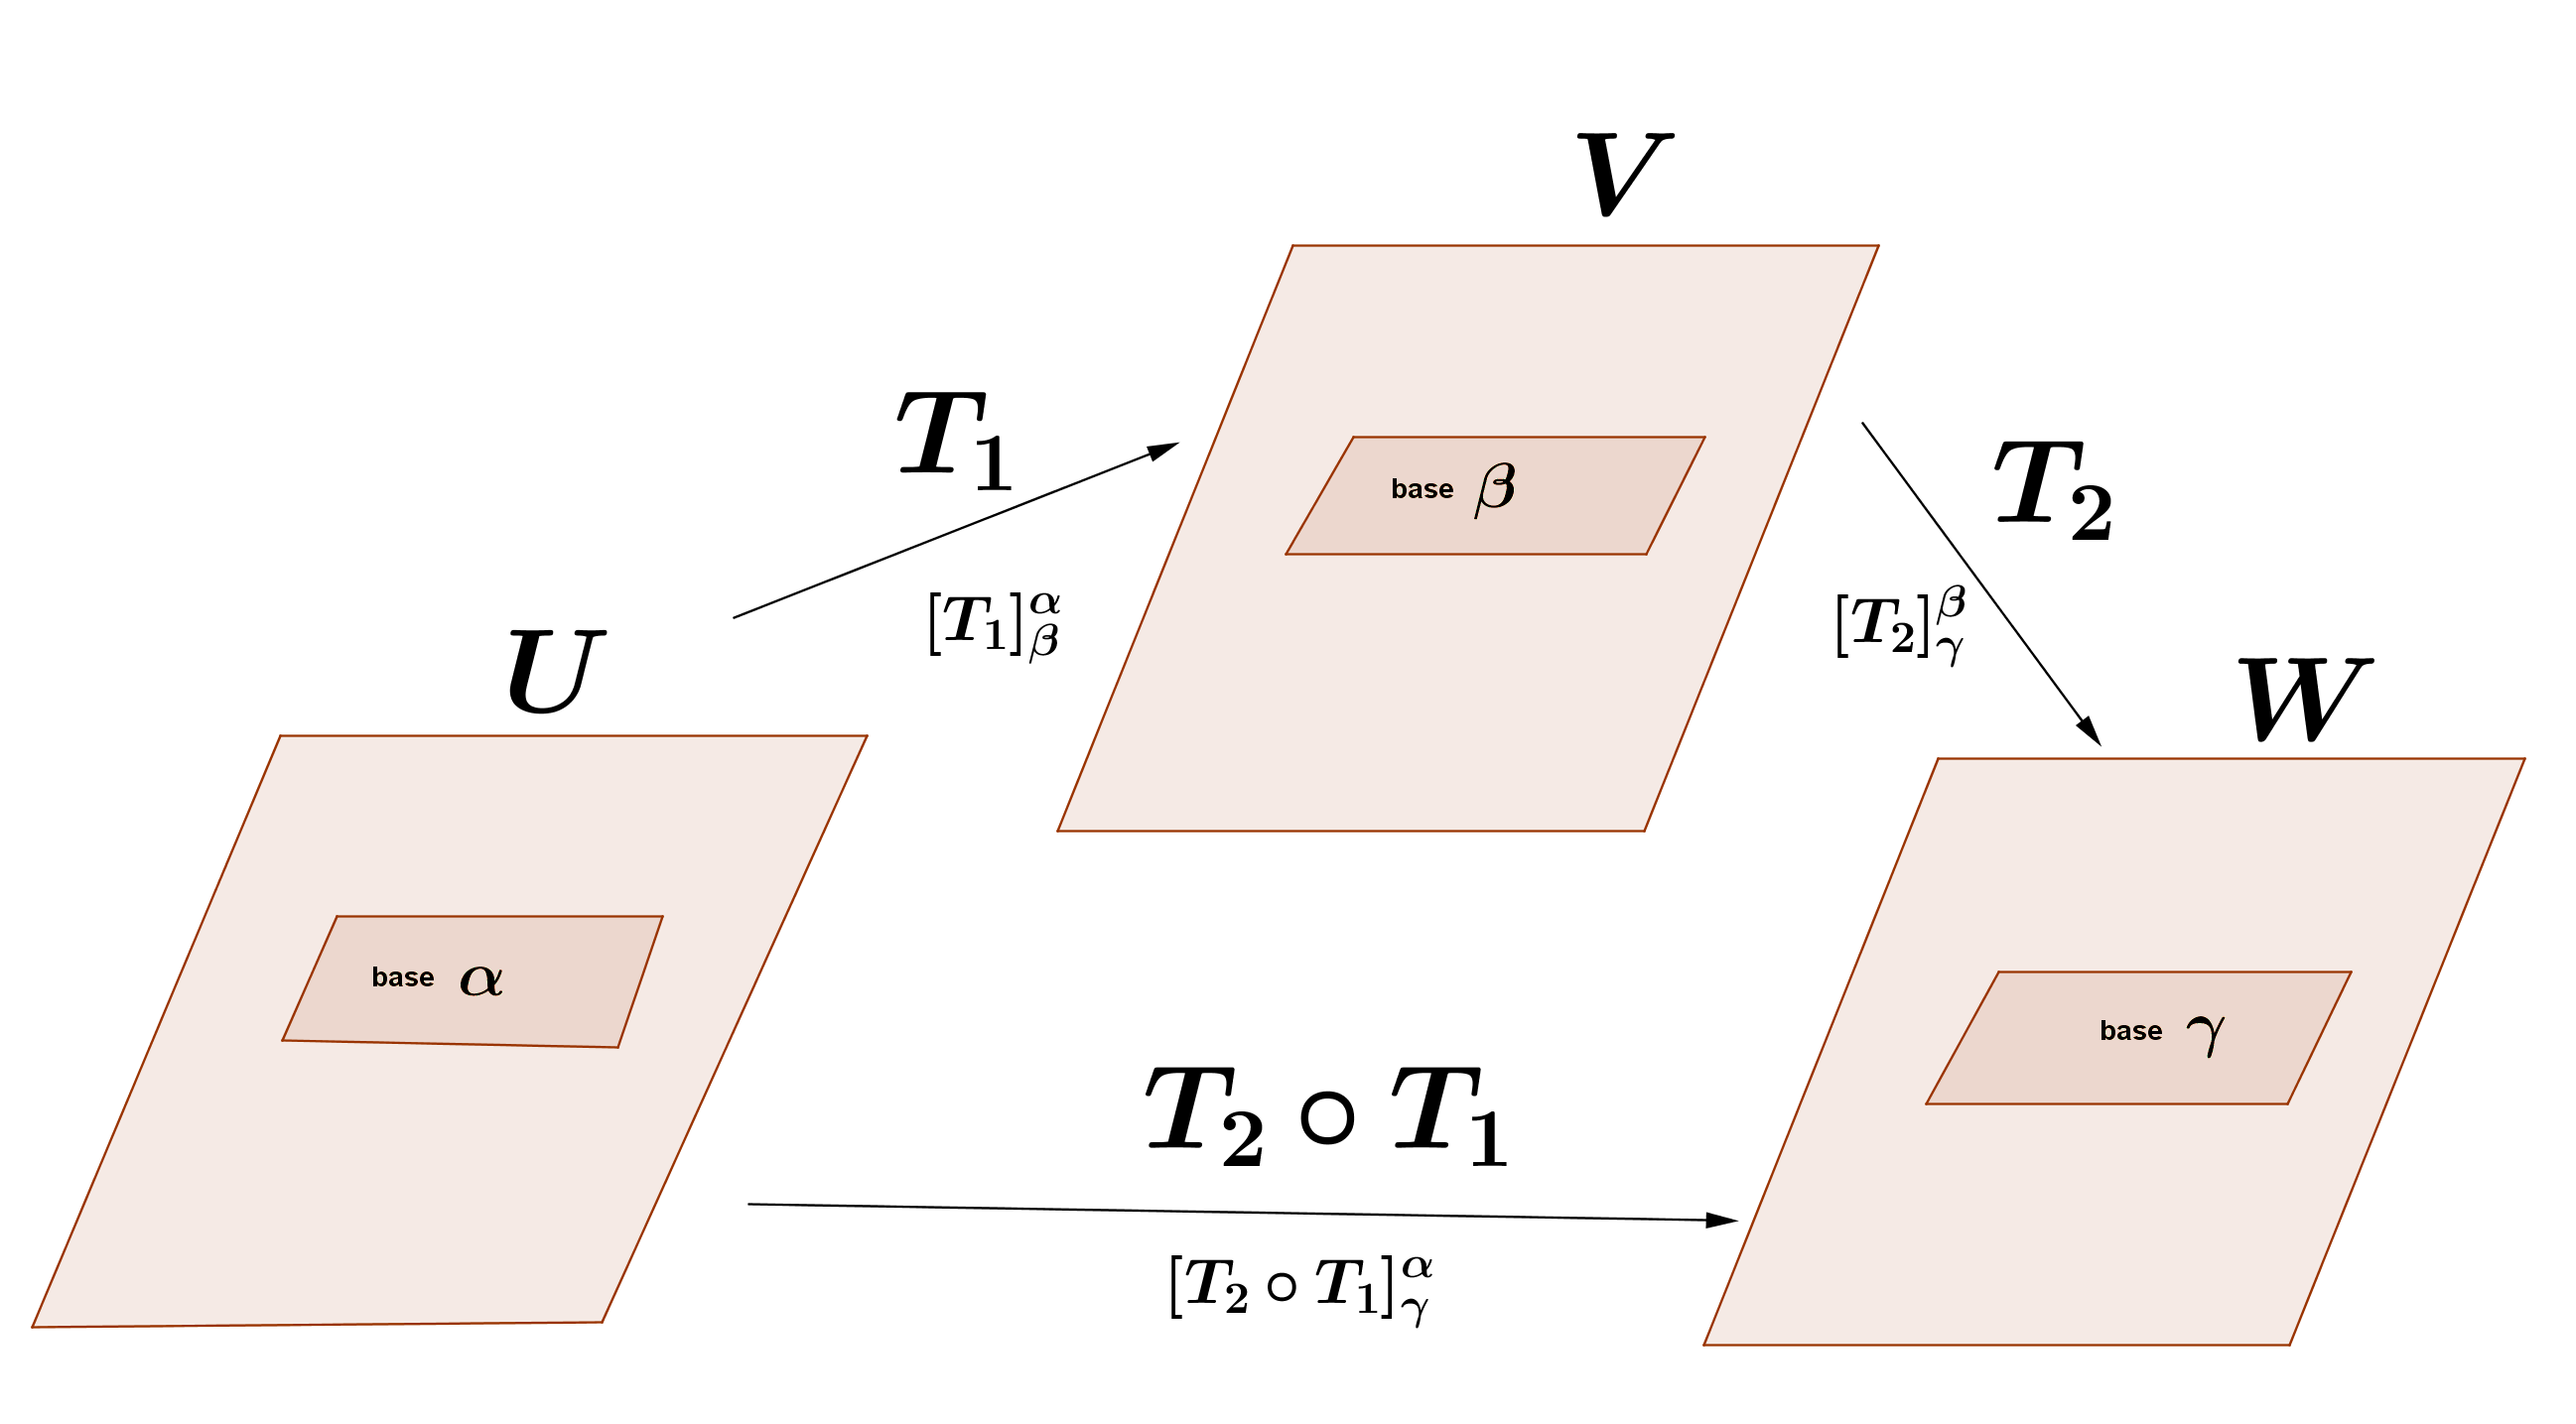
\includegraphics[width=0.8\textwidth]{chapters/matriz_trans_linear/img/composicao}
\caption{\footnotesize{Matriz da composição de duas transformações lineares}}
\label{fig:exp}
\end{figure}


\noindent\textit{\textbf{Demonstração.}} Queremos mostrar que $[T_2 \circ T_1]_{\gamma}^{\alpha}=[T_2 ]_{\gamma}^{\beta} \cdot[T_1]_{\beta}^{\alpha}$. Para isso note que pelo \textbf{Teorema 1} temos
\begin{equation}
[(T_2 \circ T_1)(u)]_{\gamma}=[T_2 \circ T_1]_{\gamma}^{\alpha}[u]_{\alpha}\;\;  e \;\; [(T_2 ( T_1(u))]_{\gamma}=[T_2 ]_{\gamma}^{\beta}[T_1(u)]_{\beta}. \label{teo21}
\end{equation}

Como $(T_2 \circ T_1)(u)=(T_2 ( T_1(u))$, segue  que
\begin{equation}
[T_2 \circ T_1]_{\gamma}^{\alpha}[u]_{\alpha}=[T_2 ]_{\gamma}^{\beta}[T_1(u)]_{\beta}.\label{teo22}
\end{equation}

Mas, por outro lado, também pelo \textbf{Teorema 1}, vem que

\begin{equation}
[T_1(u)]_{\beta}=[T_1]_{\beta}^{\alpha}[u]_{\alpha}.\label{teo23}
\end{equation}

Substituindo \eqref{teo23} em \eqref{teo22}, obtemos:
\begin{equation}
[T_2 \circ T_1]_{\gamma}^{\alpha}[u]_{\alpha}=[T_2 ]_{\gamma}^{\beta}[T_1]_{\beta}^{\alpha}[u]_{\alpha}.\label{teo24}
\end{equation}

Pela unicidade das coordenadas do vetor $u$ em relação a base $\alpha$, segue que
\begin{equation*}
[T_2 \circ T_1]_{\gamma}^{\alpha}=[T_2 ]_{\gamma}^{\beta}[T_1]_{\beta}^{\alpha},
\end{equation*}
como queríamos demonstrar.

\vspace{0.5cm}
Como consequência do \textbf{Teorema 2} resulta que se $T$  é uma transformação linear inversível, então a matriz da transformação inversa $T^{-1}$  pode ser obtida calculando a matriz inversa  da matriz de $T$. Isso é o que afirma o próximo corolário.

\vspace{0.5cm}
\noindent\textbf{Corolário 1.} Se  $T: U \rightarrow V$  é uma transformação linear inversível, ou seja $T$ é um isomorfismo, e $\alpha$ e   $\beta$ são  bases de $U$ e $V$, então  $T^{-1}: V \rightarrow U$ é uma transformação linear e $$[T^{-1} ]_{\alpha}^{\beta} = \left( [T]_{\beta}^{\alpha}\right)^{-1}.$$



\subsection{Matrizes Semelhantes}

Seja  $T:U \rightarrow U$ uma transformação linear e considere $\alpha$ e $\beta$ bases distintas de  $U$.  Então,  podemos obter uma matriz de $T$ em relação a base $\alpha$,  $[T]_{\alpha}^{\alpha}$; e uma matriz de $T$ em relação a base $\beta$,    e  $[T]_{\beta}^{\beta}$.  Uma pergunta importante a se fazer sobre essas duas matrizes  é a seguinte: qual a relação entre as matrizes $[T]_{\alpha}^{\alpha}$ e $[T]_{\beta}^{\beta}$?

Para responder a essa questão, considere  a \textbf{Figura 3.}

\begin{figure}[h!]
\center
% \includegraphics[width=1.0\textwidth]{chapters/matriz_trans_linear/img/semelhanca1}
\caption{\footnotesize{}}
\label{fig:exp}
\end{figure}

Note que as  transformações identidade $I_1$ e $I_2$ possuem matrizes em relação as bases $\alpha$ e $\beta$, $[I_1]_{\alpha}^{\beta}$  e $ [I_2]_{\beta}^{\alpha}$, respectivamente. Note ainda que podemos escrever  $T$ como a transformação composta $$ T=I_2 \circ T \circ I_1.$$

Dessa forma, obtemos
$$ [T]_{\beta}^{\beta}=[I_2 \circ T \circ I_1]_{\beta}^{\beta}.$$

Segue do \textbf{Teorema 2} que
$$ [T]_{\beta}^{\beta}=[I_2]_{\beta}^{\alpha} [ T ]_{\alpha}^{\alpha} [ I_1]_{\alpha}^{\beta}.$$

Como $[ I_1]_{\alpha}^{\beta}=([I_2]_{\beta}^{\alpha})^{-1}$, pois são matrizes mudança de base entre as bases $\alpha$ e $\beta$ e vice-versa; fazendo $P= [I_2]_{\beta}^{\alpha}$, obtemos

$$[T]_{\beta}^{\beta}=P[ T ]_{\alpha}^{\alpha}P^{-1}.$$

Isto significa que as matrizes $[T]_{\alpha}^{\alpha}$ e $[T]_{\beta}^{\beta}$ são \textit{matrizes semelhantes}.

\vspace{0.3cm}

Dizemos que duas matrizes $A$ e $B$ de mesma ordem $n$  são semelhantes, se existe uma matriz $P$, também de  ordem $n$,   invertível  e tal que $$A=P^ {-1}BP.$$


Matrizes semelhantes são importantes porque compartilham, entre outras propriedades, a de possuirem o mesmo determinante e  os mesmos autovalores. No nosso contexto, isso significa que o determinante da matriz $[T]_{\alpha}^{\alpha}$ é igual ao determinante da matriz $[T]_{\beta}^{\beta}$, que é igual ao determinante da matriz da transformação $T$ em qualquer base de $U$. A relevância desse resultado está no fato de que podemos determinar uma  base  de $U$ na qual a matriz de $T$ possa ser a mais simples possível. Por exemplo, uma matriz diagonal.  O problema de determinar uma base do espaço vetorial $U$ para a qual a transformação linear $T:U \rightarrow U$ seja uma matriz diagonal é um problema central nesse curso e será estudado mais adiante.

\chapter{Transformações Lineares}
\thispagestyle{empty}

\section{Introdução}
O objetivo deste tópico é estudar funções (também chamadas de aplicações ou transformações) entre espaços vetoriais.  Estamos interessados particularmente em funções que preservem as operações de soma de vetores e multiplicação por escalar. As funções que satisfazem tais propriedades  são chamadas de transformações lineares. Estudaremos aqui apenas transformações lineares entre espaços vetoriais reais. No entanto, todos os conceitos apresentados são extensíveis à espaços vetoriais complexos.

\section{Transformação Linear}


\textbf{Definição (Transformação Linear).} Sejam $U$  e $V$ espaços vetoriais sobre o conjunto dos números reais.  Uma transformação linear de $U$ em $V$, $$T: U \rightarrow V$$  é uma função que possui as seguintes propriedades:
\begin{enumerate}[label=(\roman*)]
\item $T(u+v)=T(u)+T(v)$, para todo $u$ e $v$ em $U$.
\item $T(\alpha u )= \alpha T(u)$, para todo $u \in U$ e todo $\alpha \in \mathbb{R}$.
\end{enumerate}

\vspace{0.7cm}
\noindent \textbf{Observações.}

\begin{enumerate}
\item  {As propriedades $(i)$ e $(ii)$ são equivalentes à  $$ T(u+\alpha v)= T(u)+ \alpha T(v)$$ para todo $u$ e $v$ em $U$ e para todo $\alpha \in \mathbb{R}$ .}

\item Se $T: U \rightarrow V$ é uma transformação linear, então $$T(0_u)=0_v.$$
\end{enumerate}

As duas observações anteriores facilitam o trabalho de verificar se uma dada aplicação $T: U \rightarrow V$ é uma transformação linear, o que pode ser feito da seguinte maneira:  Primeiro, calculamos $T(0_u)$.    Se $T(0_u) \neq 0_v$, então  $T$ não pode ser uma transformação linear.  Agora,  caso $T(0_u)=0_v$,  então verificamos se  $T$  satisfaz $ T(u+\alpha v)= T(u)+ \alpha T(v)$ para todo $u$ e $v$ em $U$ e para todo $\alpha \in \mathbb{R}$. Em caso afirmativo, concluímos que $T$ é uma transformação linear de $U$ em $V$.

\vspace{0.3cm}

\section{Exemplos de Transformações Lineares}
\begin{enumerate}
\item A aplicação $T: \mathbb{R}^2 \rightarrow \mathbb{R}$ definida por $T(x,y)=x+y$ é uma transformação linear. De fato, $T(0,0)=0+0=0$. Além disso, sejam $u=(x_1,y_1)$ e $v=(x_2,y_2)$ vetores quaisquer do $\mathbb{R}^2$ e $\alpha$ um  número real qualquer. Note que $$u+ \alpha v=(x_1+\alpha x_2, y_1+\alpha y_2). $$  Assim,  $$T(u+\alpha v)=T(x_1+\alpha x_2, y_1+\alpha y_2)=(x_1+\alpha x_2)+ (y_1+\alpha y_2)=(x_1+y_1)+\alpha ( x_2+y_2).$$ Por outro lado, como $T(u)= x_1+y_1$ e $T(v)=x_2+y_2$, então  $$T(u)+ \alpha T(v)= x_1+y_1+ \alpha(x_2+y_2).$$ Portanto,
$ T(u+\alpha v)= T(u)+ \alpha T(v)$.

\item A aplicação $T: \mathbb{R}^2 \rightarrow \mathbb{R}^2$ definida por $T(x,y)=(x+y, x+1)$ não  é uma transformação linear. De fato, $T(0,0)=(0,1) \neq (0,0)$.

\item A aplicação $T: \mathbb{R}^2 \rightarrow \mathbb{R}^3$ definida por $T(x,y)=(x,x+y,y)$ é uma transformação linear. De fato, $T(0,0)=(0,0,0)$. Além disso, sejam $u=(x_1,y_1)$ e $v=(x_2,y_2)$ vetores quaisquer do $\mathbb{R}^2$ e $\alpha$ um  número real qualquer.  $$T(u+\alpha v)=T(x_1+\alpha x_2, y_1+\alpha y_2)=(x_1+\alpha x_2, x_1+\alpha x_2+ y_1+\alpha y_2,  y_1+\alpha y_2). $$ Por outro lado,   como $T(u)=(x_1,x_1+y_1,y_1$ e $T(v)=(x_1, x_2+y_2, y_2)$, então    $$T(u)+\alpha T(v)=(x_1, x_1+y_1, y_1)+\alpha ( x_2,  x_2+y_2, y_2)=(x_1+\alpha  x_2, x_1+y_1+ \alpha ( x_2+ y_2), y_1 + \alpha y_2).$$   Portanto, $T(u+\alpha v)=T(u)+\alpha T(v).$

\item A aplicação $T: \mathbb{R}^3 \rightarrow \mathbb{R}^3$ definida por $T(x,y, z)=(x,y,z)$ é uma transformação linear. De fato, $T(0,0, 0)=(0,0,0)$. Além disso, sejam $u=(x_1,y_1, z_1)$ e $v=(x_2,y_2, z_2)$ vetores quaisquer do $\mathbb{R}^3$ e $\alpha$ um  número real qualquer.  Note que $$u+ \alpha v=(x_1+\alpha x_2, y_1+\alpha y_2, z_1+\alpha z_2). $$
Dessa  maneira,
 $$T(u+\alpha v)=T(x_1+\alpha x_2, y_1+\alpha y_2, z_1+\alpha z_2)=(x_1+\alpha x_2, y_1+\alpha y_2, z_1+\alpha z_2). $$ Por outro lado, $$T(u)+\alpha T(v)=(x_1, x_1, z_1)+\alpha ( x_2,  x_2, z_2)=(x_1+\alpha x_2, y_1+\alpha y_2, z_1+\alpha z_2).$$ Portanto, $ T(u+\alpha v)=T(u)+\alpha T(v)$.

\item  A aplicação $T: \mathbb{R}^3 \rightarrow \mathbb{M}(2, 2)$ definida por $$T(x,y, z)= \left[ \begin{array}{cc} x & 3\\ x-y & z-x \end{array} \right]$$  não  é uma transformação linear. De fato, $T(0,0, 0)= \left[ \begin{array}{cc} 0 & 3\\ 0 & 0 \end{array} \right] \neq \left[ \begin{array}{cc} 0 & 0\\ 0 & 0 \end{array} \right]$.

\item  A aplicação $T: \mathbb{R}^2 \rightarrow \mathbb{R}^2$ definida por $$T(x,y)=(xcos\theta - ysen\theta,xsen\theta+ ycos\theta)$$
% \left[ \begin{array}{cc} xcos\theta & ysen\theta \\ -xsen\theta & ycos\theta \end{array} \right]$$
é uma transformação linear. Com efeito, dados  $u=(x_1,y_1)$ e $v=(x_2,y_2)$ vetores quaisquer do $\mathbb{R}^2$ e $\alpha \in \mathbb{R}$, temos:

\begin{align*}
T(u+\alpha v) &= T(x_1+\alpha x_2, y_1+\alpha y_2) \\
                        &= ((x_1+\alpha x_2)cos\theta - (y_1+\alpha y_2)sen\theta, (x_1+\alpha x_2)sen\theta+ (y_1+\alpha y_2)cos\theta)\\
                       &=  (x_1cos\theta - y_1sen\theta, x_1sen\theta+ y_1cos\theta)+(\alpha x_2cos\theta - \alpha y_2sen\theta, \alpha x_2sen\theta+ \alpha y_2cos\theta)\\
                      &=  (x_1cos\theta - y_1sen\theta, x_1sen\theta+ y_1cos\theta)+\alpha( x_2cos\theta -  y_2sen\theta,  x_2sen\theta+ y_2cos\theta))\\
                       &=T(u)+\alpha T(v).
%\left[ \begin{array}{cc} (x_1+\alpha x_2)cos\theta & (y_1+\alpha y_2) sen\theta \\ -(x_1+\alpha x_2)sen\theta & (y_1+\alpha y_2)cos\theta \end{array} \right] \\
%&=  ((x_1+\alpha x_2)cos\theta - (y_1+\alpha y_2)sen\theta, (x_1+\alpha x_2)sen\theta+ (y_1+\alpha y_2)cos\theta)\\ %\left[ \begin{array}{cc} x_1cos\theta & y_1 sen\theta \\ -x_1sen\theta & y_1cos\theta \end{array} \right] + \alpha \left[ \begin{array}{cc}  x_2cos\theta & y_2 sen\theta \\ -x_2sen\theta & y_2cos\theta \end{array} \right]\\
%&=T(u)+\alpha T(v).
\end{align*}


\item A aplicação $T: \mathcal{P}_2(\mathbb{R}) \rightarrow \mathbb{R}^3$ definida por $$T(a_0+a_1x+a_2x^2)=(a_0, a_1, a_2)$$ é uma transformação linear. Com efeito, sejam $p(x)=a_0+a_1x+a_2x^2$ e $q(x)=b_0+b_1x+b_2x^2$ polinômios quaisquer do espaço vetorial $\mathbb{P}_2(\mathbb{R})$ e $\alpha \in \mathbb{R}$.  Da soma de dois polinômios obtemos $$p+\alpha q=a_0+\alpha b_0+(a_1+\alpha b_1)x+(a_2+\alpha b_2)x^2.$$ Assim, $$T(p+\alpha q)=T(a_0+\alpha b_0+(a_1+\alpha b_1)x+(a_2+\alpha b_2)x^2)=(a_0+\alpha b_0, a_1+\alpha b_1, a_2+\alpha b_2).$$
Por outro lado, como $T(p)=(a_0, a_1,a_2)$ e $T(q)=(b_0, b_1, b_2))$, então  $$T(p) +\alpha T(q)=(a_0, a_1, a_2) + \alpha ( b_0, b_1, b_2)=(a_0+\alpha b_0, a_1+\alpha b_1, a_2+\alpha b_2).$$ Logo, $ T(p+\alpha q)=T(p)+\alpha T(q)$.

\item Seja $D: \mathcal{P}_3(\mathbb{R}) \rightarrow \mathcal{P}_2(\mathbb{R})$ uma transformação do espaço dos polinômios de grau menor ou igual a 3 no espaço dos polinômios de grau menor ou igual a 2, ambos sobre $\mathbb{R}$, tal que $$D(a_3x^3+a_2x^2+a_1x+a_0)=3a_3x^2+2a_2x+a_1.$$ Isto é, $\mathcal{D}$ é a função derivada restrita ao espaço vetorial $\mathcal{P}_3(\mathbb{R})$. Como a derivada da soma de duas funções é a soma das derivadas dessas funções; e a derivada do produto de uma constante por uma função é igual a constante vezes a derivada da função, então podemos afirmar que $D$ é uma transformação linear de $\mathcal{P}_3(\mathbb{R})$ em $ \mathcal{P}_2(\mathbb{R})$.

\item Seja $\mathcal{C}([a,b], \mathbb{R})$ o conjunto formado por todas as funções reais  $f: [a,b] \rightarrow \mathbb{R}$ contínuas em $[a,b]$. A transformação  $S: \mathcal{C}([a,b], \mathbb{R}) \rightarrow \mathbb{R}$ tal que $$S(f)=\int_{a}^{b}f(x)dx$$ é uma transformação linear. De fato, a constatação deste fato é uma consequências das propriedades das integrais definidas.
\end{enumerate}

%\section{Exercícios Propostos}
\section{Exercícios Propostos}
\begin{enumerate}
\item Seja $V$ um espaço vetorial real qualquer. Mostre que $T: V \rightarrow V$   dada por $T(v)=v$ é uma transformação linear.

\item Seja $T: \mathbb{R} \rightarrow  \mathbb{R}$ uma aplicação definida por $T(x)=\lambda x$. Mostre que $T$ é linear. (Na verdade,  toda transformação linear de  $\mathbb{R}$ em $ \mathbb{R}$ é da forma $\lambda x$. Mostre isso!).
\item Mostre que as seguintes aplicações de $\mathbb{R}^2$ em $\mathbb{R}^2$ são transformações lineares.

\begin{enumerate}[label=(\alph*)]
\item  $T: \mathbb{R}^2 \rightarrow \mathbb{R}^2$ definida por $T(x,y)=c(x,y)$ para todo $c \in \mathbb{R}$ (\textit{Contração ou expansão}).
\item  $T: \mathbb{R}^2 \rightarrow \mathbb{R}^2$ definida por $T(x,y)=(x,-y)$  (\textit{Reflexão em torno do eixo x}).
\item  $T: \mathbb{R}^2 \rightarrow \mathbb{R}^2$ definida por $T(x,y)=(-x,-y)$  (\textit{Reflexão na origem}).
\item  $T: \mathbb{R}^2 \rightarrow \mathbb{R}^2$ definida por $T(x,y)=(x+cy,y)$ para todo $c \in \mathbb{R}$ (\textit{Cisalhamento horizontal}).
\end{enumerate}

\item Sejam $a$ e $b$ números reais diferentes de zero.  Mostre que  $T: \mathbb{R}^2 \rightarrow \mathbb{R}^2$ definida por $T(x,y)=(x+a,y+b)$ (\textit{Translação}) não é uma transformação linear.

\item  Mostre que a aplicação $T: \mathbb{R}^2 \rightarrow \mathbb{M}(2, 2)$ definida por $$T(x,y)= \left[ \begin{array}{cc} x+y & x\\ y & x-y \end{array} \right]$$   é uma transformação linear.



\item Seja $P \in \mathbb{M}(2, 2)$ uma matriz invertível e $T_P: \mathbb{M}(2, 2) \rightarrow \mathbb{M}(2, 2)$, definida por $$T_P(X)=P^{-1}XP.$$ Mostre que $T_P$ é linear.

\item Sejam $U$ e $V$ espaços vetoriais  quaisquer.  Se  $T: U \rightarrow V$   é uma transformação linear, mostre que $T(0_u)=0_v$.

\item {Sejam $V$ e $W$ espaços vetoriais  sobre $\mathbb{R}$ e $T : V \rightarrow W$ uma transformação linear. Mostre que se  $\{T(v_1),T( v_2),...,T(v_n)\}$ é um conjunto linearmente independente de $W$, então $\{v_1, v_2,...,v_n\}$ é um conjunto linearmente independente de $V$.}

\end{enumerate}

\section{Determinando uma transformação linear a partir da imagem dos vetores de uma base do domínio}
 Uma característica muito importante das transformações lineares é que uma transformação linear fica univocamente determinada se conhecemos seus valores nos vetores de uma base do domínio. Esse resultado é consequência do seguinte teorema:

\vspace{0.3cm}
\noindent \textbf{Teorema 1.} \textit{Sejam $\{ u_1, u_2, ..., u_n\}$ uma base de um espaço vetorial  $U$. Sejam $\{ v_1, v_2,..., v_n\}$ vetores de um espaço vetorial $V$. Então, existe uma única transformação linear  $T: U \rightarrow V$ tal que $T(u_i)=v_i$ para $i=1,2, ..., n$. }

\vspace{0.3cm}
\noindent \textbf{Observação.} Esta aplicação é dada por: se $$ u=a_1u_1+a_2u_2+...+a_nu_n,$$  então  $$T(u)=a_1T(u_1)+a_2T(u_2)+...+a_nT(u_n)=a_1v_1+a_2v_2+...+a_nv_n.$$

Além de afirmar a existência de uma única transformação linear satisfazendo certas condições, o teorema anterior, e a observação anterior, nos fornecem um roteiro de como determinar uma transformação linear $T: U \rightarrow V$ conhecendo-se uma base de $U$,  $\{ u_1, u_2, ..., u_n\}$, e  $n$ vetores de $V$, $\{ v_1, v_2,..., v_n\}$ , tais que $T(u_i)=v_i$ para $i=1,2, ..., n$.
\begin{enumerate}
\item Certifique-que $u_1, u_2,...,u_n$ formam uma base de $U$;
\item Escreva um vetor genérico de  $u \in U$ como uma combinação linear de $u_1, u_2,...,u_n$. Isto é, calcule escalares $a_1, a_2,...,a_n$ tais que $$u=a_1u_1+ a_2u_2+...+a_nu_n;$$
\item Escreva a equação $T(u)=a_1T(u_1)+ a_2T(u_2)+...+a_nT(u_n)$;
\item Faça a substituição $T(u_i)=v_1$ para $i=1,2,...,n$.
\item Organize os cálculos e escreva a expressão para $T(u)$,  onde $u$ é um vetor qualquer de $U$.
\end{enumerate}

\section{ Exemplo}
Dada uma base qualquer de $\mathbb{R}^2$, por exemplo, $\beta=\{(1,1), (-1, 1)\}$,  e dois vetores quaisquer de  $\mathbb{R}^3$, por exemplo, $( 1, -1,1)$ e $(0, 1,2)$.  O teorema anterior afirma que existe uma única transformação linear $T: \mathbb{R}^2 \rightarrow \mathbb{R}^3$ tal que $$T(1,1) = (1, -1, 1)$$ e  $$T(-1, 1) =(0, 1, 2).$$
Além disso, como dado $(x,y) \in \mathbb{R}^2$, sempre vai existir escalares $a_1$ e $a_2$ únicos, tais que,  $(x,y)= a_1(1, 1)+ b_1(-1, 1)$, então  a  transformação linear $T$ é dada por $$T(x,y)= a_1T(1, 1)+ b_1T(-1, 1)= a_1(1,-1,1)+a_2(0, 1,2).$$
Dessa maneira, para encontrarmos uma fórmula para $T$ basta apenas calcularmos os escalares $a_1$ e $a_2$. Isso pode ser feito, resolvendo-se o sistema $$(x,y)= a_1(1, 1)+ b_1(-1, 1).$$
Ou seja,
\begin{align*}
x &=a_1-b_1 \\
y&=a1+b1.
\end{align*}

Daí  obtemos $a_1=\dfrac{x+y}{2}$ e $a_2=\dfrac{y-x}{2}$. Dessa maneira,
\begin{align*}
T(x,y)&= \dfrac{x+y}{2}(1,-1,1)+\dfrac{y-x}{2}(0, 1,2)\\
          &=\left(\dfrac{x+y}{2}, -x, \dfrac{-x+3y}{2}\right).
\end{align*}

Portanto, a transformação linear procurada é



 $$T(x,y)= \left(\dfrac{x+y}{2}, -x, \dfrac{-x+3y}{2}\right).$$

\section{Exercícios Propostos}
\begin{enumerate}

\item Seja $T: \mathbb{R}^2 \rightarrow \mathbb{R}^2$  uma transformação linear tal que $T(1,0)=(1,1)$ e $T(0,1)=(-1,1)$.
\begin{enumerate}[label=(\alph*)]
\item Determine $T(x,y)$.
\item Calcule $T(2,3)$.
%\item Descreva $Ker(T)$ e $Im(T)$.
\end{enumerate}

\item Seja $T: \mathbb{R}^3 \rightarrow \mathbb{R}^3$  uma transformação linear tal que $T(1,0,0)=(2,-1,1)$,  $T(1,1, 0)=(-1,2,1)$  e $T(1,1, 1)=(1,1,-2)$ .
\begin{enumerate}[label=(\alph*)]
\item Determine $T(x,y,z)$.
\item Calcule $T(2,3,1)$.
%\item Descreva $Ker(T)$ e $Im(T)$.
\end{enumerate}

\item Seja  Seja $T: \mathbb{R}^3 \rightarrow \mathbb{R}$ tal que  $T(1,-1,1)=1$,  $T(1,0, 2)=2 $  e $T(1,1, 1)=3$ . Determine $T(x,y,z)$.
%\begin{enumerate}[label=(\alph*)]
%\item  $T(x,y)$.
%\item $Ker(T)$.
%\end{enumerate}

\item Seja $T: \mathbb{R}^4 \rightarrow \mathbb{R}^2$  uma transformação linear tal que  $T(1,0,0, 0)=(1,1)$, $T(1,1,0,0)=(-1,1)$,  $T(0,1,1, 0)=(1,-1)$ e   $T(0,0,1, 1)=(-1,-1)$ .
\begin{enumerate}[label=(\alph*)]
\item Determine $T(x,y,z,t)$.
\item Calcule $T(1,2,2,3)$.
%\item Descreva $Ker(T)$ e $Im(T)$.
\end{enumerate}

\item Seja $T: \mathbb{P}_2(\mathbb{R}) \rightarrow \mathbb{R}^3$  uma transformação linear tal que  $T(1+2x+x^2)=(1,2,1)$, $T(1+x)=(1,-1,-2)$ e  $T(2)=(1,0,0)$. Determine $T(a_0+a_1x+a_2x^2)$.
\end{enumerate}

\section{Núcleo e Imagem}
\textbf{Definição (Núcleo e Imagem).} \textit{Sejam $U$  e $V$ espaços vetoriais e $T: U \rightarrow V$ uma transformação linear. }

\begin{enumerate}%[label=(\roman*)]
\item \textit{O conjunto $\{ u\in U; \;T(u)=0_v\}$ é chamado de \textit{Núcleo de $T$} e será denotado por \textit{Ker(T)}.}

\begin{figure}[h]
\center
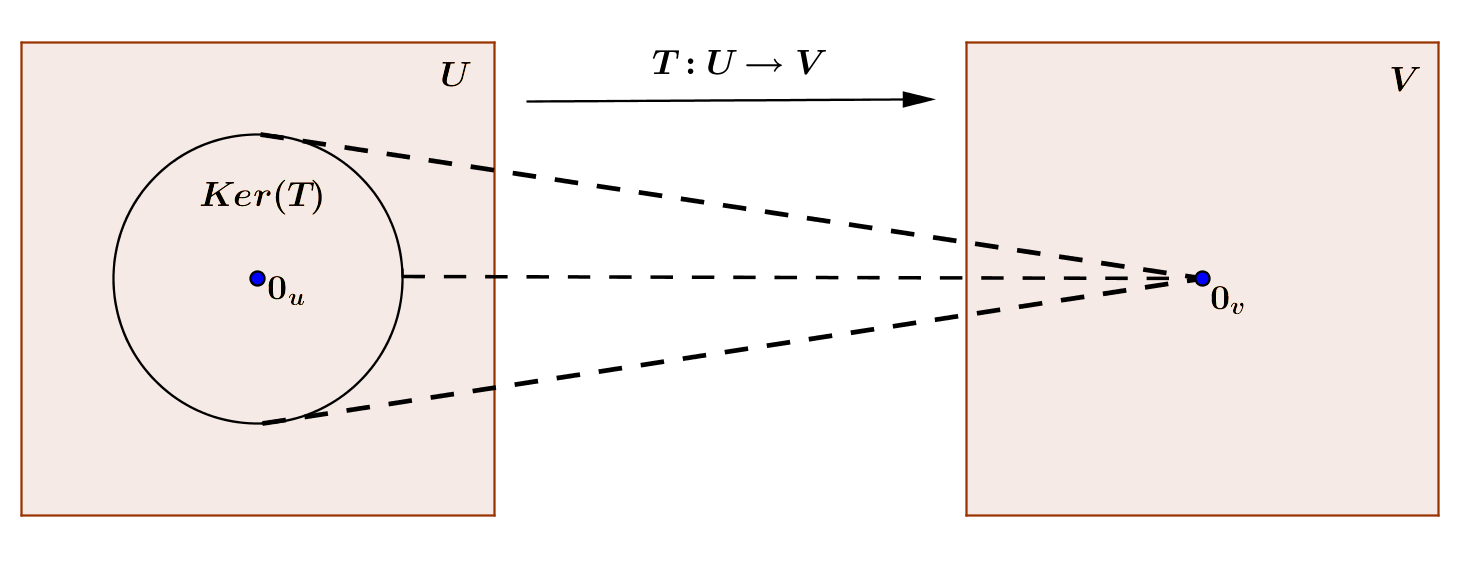
\includegraphics[width=0.70\textwidth]{chapters/transformacoes_lineares/img/kert1}
\caption{\footnotesize{Cada vetor $u \in Ker(T)$ é levado  em $0_v$ por  T .}}
\label{fig:exp}
\end{figure}


\item \textit{O conjunto $\{ v \in V;  \; v=T(u) \; \; \text{para algum}\; u\in U\}$ é chamado de \textit{Imagem de $T$} e será denotado por \textit{Im(T)}, ou simplesmente $T(U)$.}

\begin{figure}[h!]
\center
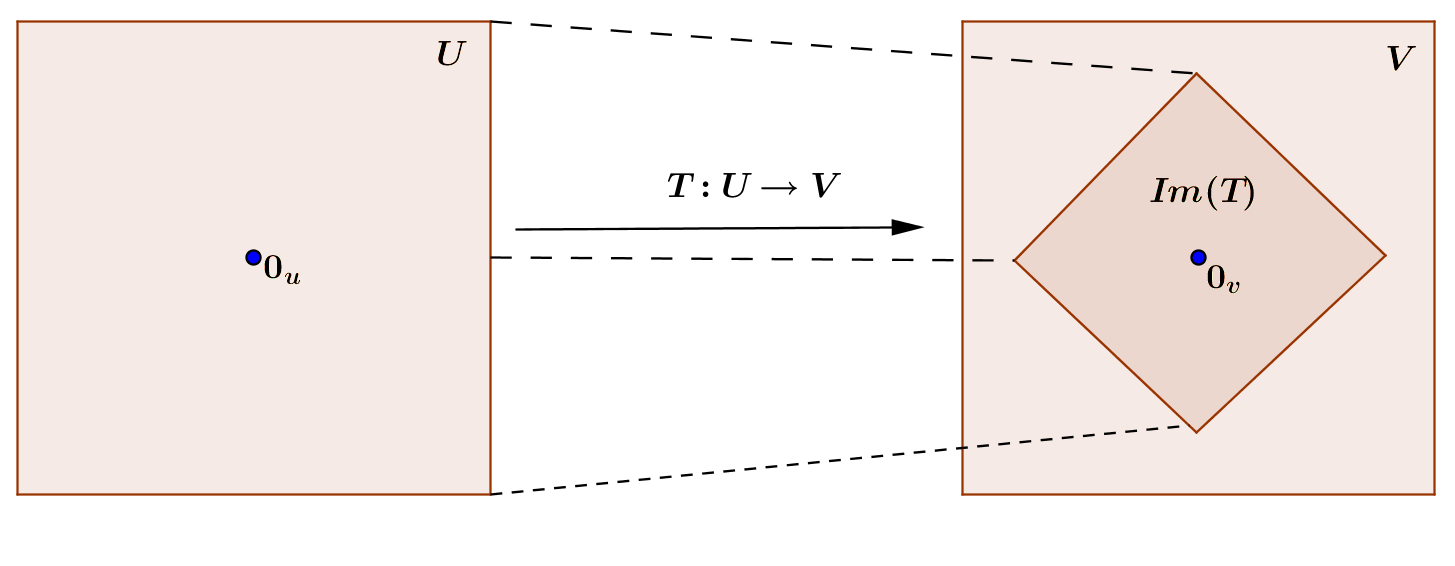
\includegraphics[width=0.70\textwidth]{chapters/transformacoes_lineares/img/imt1}
\caption{\footnotesize{Representação gráfica da imagem de T.}}
\label{fig:exp}
\end{figure}

\end{enumerate}

Observe que tanto \textit{Ker(T)} como \textit{Im(T)} são conjuntos diferentes do vazio. Isto porque, como já  sabemos,  $T(0_u)=0_v$. Logo, cada um desses conjuntos têm pelo menos o elemento nulo. Dessa forma, é conveniente investigar se esses conjuntos possuem a estrutura de um espaço vetorial. A resposta a essa pergunta é dada pelo \textbf{Teorema 2}.





\vspace{1cm}
\noindent \textbf{Teorema 2.} \textit{Seja $T: U \rightarrow V$ uma transformação linear. Então, \textit{Ker(T)} é um subespaço vetorial de $U$ e \textit{Im(T)} é um subespaço vetorial de $V$.}

\noindent \textbf{Demonstração.} Primeiro vamos mostrar que \textit{Ker(T)} é um subespaço vetorial de $U$. Para isso, sejam $u_1$ e $u_2$ dois vetores quaisquer de  \textit{Ker(T)} e $\lambda \in \mathbb{R}$. Vamos mostrar que $u_1+\lambda u_2 \in{Ker(T)} $. De fato, $$T(u_1+\lambda u_2)=T(u_1)+\lambda T(u_2)$$ pois $T$ é linear. Mas, como $u_1$ e $u_2$ pertencem  a  \textit{Ker(T)},  temos $T(u_1)=0_v$ e $T(u_2)=0_v$. Daí, $$T(u_1+\lambda u_2)=0_v+\lambda 0_v=0_v.$$ Logo,   $u_1+\lambda u_2 \in{Ker(T)} $ e, portanto, \textit{Ker(T)} é um subespaço vetorial de $U$.

Agora para mostrar que \textit{Im(T)} é um subespaço vetorial de $V$, considere dois vetores genéricos  $v_1$ e $v_2$ em \textit{Im(T)}. Daí, pela definição da \textit{Im(T)}, existem vetores $u_1$ e $u_2$ no domínio da transformação tais que
$$v_1=T(u_1) \; \text{e} \; v_2=T(u_2).$$

Assim, para todo $\lambda \in \mathbb{R}$, temos $$v_1+\lambda v_2=T(u_1) +\lambda T(u_2).$$ Como $T$ é linear, então
$$v_1+\lambda v_2=T(u_1 +\lambda u_2).$$ Isso mostra que $v_1+\lambda v_2 \in Im(T)$, pois é imagem do vetor $u_1 +\lambda u_2 \in U$. Portanto, $Im(T)$ é um subespaço vetorial de $V$.

\vspace{1cm}

A seguir veremos como calcular o núcleo e a imagem de uma transformação linear por meio de alguns exemplos.

\section{Exemplos}
\begin{enumerate}
\item Considere a transformação linear $T: \mathbb{R}^2 \rightarrow \mathbb{R}^4$ definida por $$T(x,y)=(x, y,x+y, x-y).$$  Para determinar  $Ker(T)$  note que  $(x,y) \in Ker(T)$ se, e somente se, $T(x,y)=(0,0)$. Mas isso implica em $(x, y, x+y, x-y)=(0,0,0,0)$. Logo, devemos ter $x=0$, $y=0$, $x+y=0$ e $x-y=0$. Obviamente, $x=y=0$. Assim obtemos,  $$Ker(T)=\{(0,0)\}.$$ Agora, para calcular $Im(T)$, note que cada elemento de $\mathbb{R}^4$ que está na imagem de $T$ é dado pela transformação $T(x,y)=(x, y, x+y, x-y)$.  Assim, fazemos $$(x,y,x+y, x-y)=x(1,0,1,1)+y(0,1,1,-1).$$ Dessa maneira, $$Im(T)=[(1,0,1,1),(0,1,1,-1)].$$

\item Considere a  transformação linear $T: \mathbb{R}^3 \rightarrow \mathbb{R}^2$ definida por $T(x,y,z)=(x, y)$. O vetor $(x,y,z) \in Ker(T)$ se, e somente se, $T(x,y,z)=(0,0)$. Mas isso implica em $(x, y)=(0,0)$. Logo, devemos ter $x=0$ e $y=0$. Mas, não encontramos nenhuma restrição sobre a variável  $z$. Ou seja, $z$ é  livre. Assim obtemos,  $$Ker(T)=\{(0,0, z); \; z \in \mathbb{R}\}.$$

Já $Im(T)$ pode ser obtida através de $$T(x, y)=(x,z)=x(1,0)+y(0,1).$$ Logo, $$Im(T)=[(1,0), (0,1)]=\mathbb{R}^2.$$
\end{enumerate}

\section{Exercícios Propostos}
\begin{enumerate}
\item  Para cada uma das transformações lineares dos exercícios da \textbf{Seção 6}
\begin{enumerate}[label=(\alph*)]
\item Calcular $Ker(T)$.
\item Descrever $Im(T)$.
\end{enumerate}
\item Determine o núcleo e a imagem da transformação linear $T: \mathbb{R}^4 \rightarrow \mathbb{R}^2$ definida  por $T(x,y,z,w)=(x-y, y-z, z-w)$.

\item Demonstre o Teorema 2.
\end{enumerate}

\section{Transformações Lineares Injetivas e Sobrejetivas}

Uma função  $T: U \rightarrow V$ é \textit{injetiva} (ou injetora)  se  $$T(x)=T(y) \Rightarrow x=y,\; \text{para todo}\; x, y \in U.$$ Isto equivale a dizer que numa função injetiva  as imagens de elementos distintos são distintas.

 Por outro lado, $T$ é uma função \textit{sobrejetiva} (ou sobrejetora) se $Im(T)=V$. Isto é, todo elemento do contradomínio $V$ é  imagem de algum elemento do domínio $U$. Se uma função $T$ é injetiva e sobrejetiva,  dizemos que $T$ é \textit{bijetiva} (ou bijetora).

Por exemplo, a função $f: \mathbb{R} \rightarrow \mathbb{R}$ dada por $f(x)=x^2$ não é injetora, pois $f(-2)=f(2)=4$. Ou seja, dois elementos distintos do domínio, -2 e 2,  possuem a mesma imagem 4.  Esta função também não  é sobrejetiva, pois $f(x)=x^2 \geq 0$ para todo $x\in \mathbb{R}$. Logo, $Im(f)=[0, \infty) \neq \mathbb{R}$. Já a função $f: \mathbb{R} \rightarrow \mathbb{R}$ dada por $f(x)=x^3$ é injetiva e sobrejetiva. Com efeito, $$f(x)=f(y) \Rightarrow x^3=y^3 \Rightarrow x^3 - y^3=0 \Rightarrow (x-y)(x^2+xy+y^2)=0$$ como $x^2+xy+y^2 > 0$ sempre que $x^2+y^2 \neq 0$, então $x-y=0$. Logo, $x=y$ e portanto $f$ é injetora. É simples verificar que $Im(f)=\mathbb{R}$, logo $f$  é sobrejetiva.

\vspace{1cm}
A tarefa de identificar se uma função $T$ é injetiva, em  geral, é  mais simples se $T$ é uma transformação linear.  Isso porque, conforme o \textbf{Teorema 3} que será apresentado a seguir, o trabalho de identificar se $T$ é injetiva fica reduzido a calcular o $Ker(T)$.  Esta  importante relação entre o núcleo de uma transformação linear e o fato da mesma  ser ou não  injetiva é estabelecida pelo seguinte teorema:

\vspace{1cm}
\noindent \textbf{Teorema 3.} \textit{Seja $T: U \rightarrow V$ uma transformação linear. Então, $T$ é uma aplicação injetiva se, e somente se, $Ker(T)=\{0_u\}.$}

\vspace{0.3cm}
\noindent \textbf{Demonstração.} Primeiro, suponha que $T$ é uma transformação linear injetiva e seja $u\in Ker(T)$. Então, por definição $T(u)=0_v$. Mas, já sabemos que  $T(0_u)=0_v$. Assim, $T(u)=T(0_u)$. Como $T$ é injetiva, $u=0_u$. Como o vetor $u$ foi tomado de modo arbitrário, segue que o único vetor no $ Ker(T)$ é o vetor nulo $0_u$. Ou seja, $ Ker(T)= \{0_u\}$.

Por outro lado, suponha que  $ Ker(T)= \{0_u\}$ e sejam vetores quaisquer $u_1$ e $u_2$ em $U$, tais que $T(u_1)=T(u_2)$. Vamos mostrar que $u_1=u_2$. De fato, se $T(u_1)=T(u_2)$, temos $T(u_1)-T(u_2)=0_v$. Mas, como $T$ é linear, segue que $T(u_1-u_2)=0_v$. Logo, $u_1-u_2 \in Ker(T)$. Mas, como $ Ker(T)= \{0_u\}$, então $u_1-u_2=0_u$. Logo, $u_1=u_2$. Portanto, de acordo com a definição de função injetiva,  $T$ é injetiva.




\vspace{1cm}

\section{Exemplos}


\begin{enumerate}
\item  A transformação linear $T: \mathbb{R}^2 \rightarrow \mathbb{R}^2$ definida por $T(x,y)=(x+2y,y)$ é injetiva. Com efeito, de acordo com a definição de núcleo $(x,y) \in Ker(T)$ se, e somente se, $T(x,y)=(0,0)$. Mas isso implica em $(x+2y, y)=(0,0)$. Logo, $x+2y=0$ e $y=0$ e assim obtemos, $x=y=0$. Portanto,  $Ker(T)=\{(0,0)\}$ e $T$ é injetiva, segundo o teorema.

\item A transformação linear $T: \mathbb{R}^3 \rightarrow \mathbb{R}$ definida por $T(x,y,z)=x+y+z$ não é injetiva. De fato, de acordo com a definição de núcleo $(x,y,z) \in Ker(T)$ se, e somente se, $T(x,y,z)=0$. Mas isso implica em $x+y+z=0$. De onde obtemos  $z=-x-y$. Assim, as variáveis $x$ e $y$ são livres e podem assumir qualquer valor real. Dessa forma   $$Ker(T)=\{(x,y, -x-y); x, y \in \mathbb{R}\} \neq \{ (0,0,0)\}.$$  Logo,  $T$ não é injetiva.

\end{enumerate}

\section{Exercícios Propostos}

\begin{enumerate}

\item Considere a transformação linear  $T: \mathbb{R}^3 \rightarrow \mathbb{R}^3$ definida por $T(x,y,z)=(x,x, z-y)$.

\begin{enumerate}[label=(\alph*)]
\item Determine $Ker(T)$. $T$ é injetiva?
\item Determine uma base para $Ker(T)$.
\item Determine uma base para $Im(T)$. Qual a dimensão de $Im(T)$.
\item $T$ é sobrejetiva?
\end{enumerate}

\item Sejam $U$ e $V$ espaços vetoriais e  $\{u_1, u_2,...,u_n\}$  um conjunto de vetores linearmente independentes de $U$. Mostre que, se $T: U \rightarrow V$ é uma transformação linear injetiva, então  $\{T(u_1), T(u_2),...,T(u_n)\}$  é um conjunto de vetores linearmente de $V$ (Isto é, transformações lineares injetivas levam conjunto LI em conjunto LI).
\end{enumerate}

\section{O Teorema do Núcleo e da Imagem. Isomorfismos}

O próximo teorema é um dos mais importantes da Álgebra Linear. Ele relaciona as dimensões do núcleo e da imagem de uma transformação linear  $T: U \rightarrow V$  com  a dimensão do espaço $U$ (o domínio da transformação linear). Esse teorema traz consequências interessantes para a análise de transformações injetivas e sobrejetivas, como veremos nas próximas seções.

\vspace{1cm}
\noindent \textbf{Teorema 4 (Teorema do Núcleo e da Imagem).} \textit{Sejam $U$ e $V$ espaços vetoriais, sendo $U$ de dimensão finita,  e  $T: U \rightarrow V$ uma transformação linear. Então, $$dim(Ker(T)) + dim(Im(T))=dim(U).$$}

\noindent\textit{Demonstração. Aula}


Para avaliarmos um pouco a importância do \textbf{Teorema 4},  considere uma transformação  linear $T: \mathbb{R}^3 \rightarrow \mathbb{R}^2$. O Teorema do Núcleo e da Imagem afirma que $$dim( \mathbb{R}^3 ) =3=dim(Ker(T))+ dim(Im(T)).$$ Isto é, a soma da dimensão do núcleo de $T$ com a dimensão da imagem de $T$ tem que ser exatamente 3. Mas, como $Im(T) \subset \mathbb{R}^2$, a dimensão da imagem de $T$ é no máximo igual a 2. Logo, a dimensão do núcleo de $T$ deve ser maior ou igual a 1. Portanto, $Ker(T)\neq \{ 0_u\}$. Dessa maneira, concluimos que  $T$ não pode ser injetora. Esse raciocínio se aplica a todas as transformações lineares  $T: U \rightarrow V$  tais que $dim(U) > dim(V)$. No caso em que $dim(U) = dim(V)$, temos o seguinte resultado:


\vspace{1cm}
\noindent\textbf{Corolário 1.} \textit{Sejam $U$  e $V$ espaços vetoriais de dimensão finita e    $T: U \rightarrow V$ uma transformação linear. Se $dim(U)=dim(V)$, então  $T$ é injetiva se, e somente se, $T$ é sobrejetiva.}

\vspace{1cm}
\noindent\textbf{Definição (Isormorfismo).} Sejam $U$  e $V$ espaços vetoriais.
\begin{enumerate}%[label=(\roman*)]
\item Se $T: U \rightarrow V$  é uma transformação linear bijetiva, $T$ é chamada de \textit{isomorfismo}.
\item Quando existe um isomorfismo  $T: U \rightarrow V$, dizemos que $U$ e $V$ são espaços vetoriais \textit{isomorfos} e denotamos $U \simeq V$.
\end{enumerate}

\begin{figure}[h]
\center
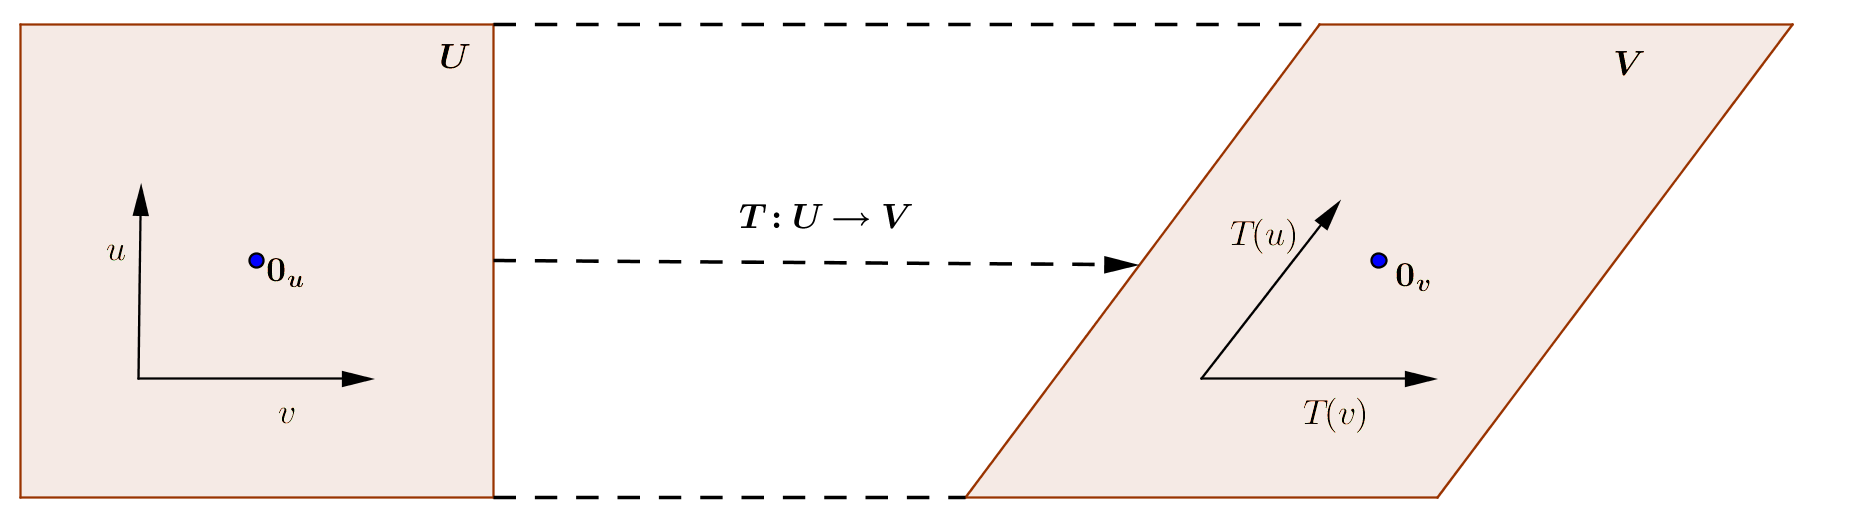
\includegraphics[width=0.70\textwidth]{chapters/transformacoes_lineares/img/isomorfismo}
\caption{\footnotesize{Espaços isomorfos possuem a mesma estrutura vetorial }}
\label{fig:exp}
\end{figure}

Espaços vetoriais isomorfos são essencialmente  iguais. A diferença está apenas na forma de representação dos seus vetores e das operações de soma de vetores e mutiplicação de vetores por escalar. Espaços vetoriais isomorfos devem ter a mesma dimensão.  Outras informações relevantes sobre isomorfismos estão resumidas na \textbf{Proposição 1}.

\vspace{1cm}
\noindent\textbf{Proposição 1.} \textit{Seja $T: U \rightarrow V$ um isomorfismo. Então, }
\begin{enumerate}%[label=(\roman*)]
\item \textit{ $T$ leva uma base de $U$ em  uma base de $V$.}
\item \textit{Existe a  aplicação inversa $T^{-1}: V \rightarrow U$ que é linear e também é um isomorfismo.}
\end{enumerate}

A \textbf{Proposição 1} apresenta uma caracterização importante dos isomorfismos: levar  base  em base. Isto é, todo isomorfismo  $T: U \rightarrow V$  transforma uma base $\{ u_1, u_2,...,u_n\}$ de $U$ no conjunto  $\{T( u_1), T(u_2),...,T(u_n)\}$ que é uma base de $V$. Dessa forma, considerando que $U$ e $V$ possuam a mesma dimensão $n$, podemos determinar a transformação linear inversa $T^{-1}: V \rightarrow U$ definindo

\begin{align*}
T^{-1}(T(u_1))&= u_1\\
T^{-1}(T(u_2))&= u_2\\
               \vdots &=\vdots\\
T^{-1}(T(u_n))&= u_n
\end{align*}

e usando o roteiro apresentado  pelo \textbf{Teorema 1}.

\vspace{1cm}
Além disso, de acordo com a \textbf{Proposição 1} podemos dizer que espaços vetoriais isomorfos  possuem a mesma dimensão. A recíproca dessa afirmação também é verdadeira. Ou seja, espaços vetoriais que possuem a mesma dimensão finita são isomorfos. Dessa maneira, como podemos ver nos exemplos a seguir, os espaços $\mathbb{R}^4$, $\mathcal{P}_3(\mathbb{R})$ e $\mathbb{M}(2,2)$  são espaços vetoriais isomorfos entre si já que todos têm dimensão 4. Isso significa que, a menos dos seus elementos, esses espaços vetoriais são idênticos. Em outras palavras, apesar dos elementos de cada um desses espaços serem diferentes (de fato, matrizes e polinômios, por exemplo, são objetos matemáticos de naturezas distintas), os espaços vetoriais isomorfos possuem a mesma estrutura. São indistinguíveis. Dessa maneira, podemos dizer que conjuntos LI de um espaço, correspondem a conjuntos LI do outro espaço, por exemplo.

\section{Exemplos}
\begin{enumerate}
\item Os espaços $\mathcal{M}(2,2)$ e $\mathbb{R}^4$ são isomorfos.  Com efeito, basta definir $T: \mathbb{R}^4 \rightarrow \mathcal{M}(2,2)$ por $$T(x,y,z,w)= \left[ \begin{array}{cc} x & y\\ z &w\end{array} \right].$$ É simples verificar que $T$ é uma transformação linear e que $Ker(T)=\{(0,0,0,0)\}$. Logo $T$ é injetiva. Como os  dois espaços possuem a dimensão,  4, então $T$ também é sobrejetiva e portanto é um isomorfismo.

\item $\mathbb{R}^4 \simeq \mathcal{P}_3(\mathbb{R})$. De fato, a aplicação $T: \mathcal{P}_3(\mathbb{R}) \rightarrow \mathbb{R}^4$ dada por $$T(a_0+a_1x+a_2x^2+a_3x^3)=(a_0, a_1, a_2, a_3, a_4)$$ é um isomorfismo entre os dois espaços. Verifique!

\item Seja $W=\{(x,y,z)\in \mathbb{R}^3; \; z=0 \}$. $W$ é isomorfo a $\mathbb{R}^2$. De fato, note que $W=[(1,0,0), (0,1,0)]$ e que $dim(W)=2$.  Agora note que $T: \mathbb{R}^2 \rightarrow \mathbb{R}^3$ definida por $$T(x,y)=(x,y,0)$$ é tal que $Im(T)=W$.  Como $dim(\mathbb{R}^2) = dim(W)=2= dim(Im(T))$, então $T$ é um isomorfismo entre $\mathbb{R}^2$ e $W$.
\end{enumerate}

\section{Exercícios Resolvidos}
\begin{enumerate}
\item Seja $T: \mathbb{R}^3 \rightarrow\mathbb{R}^3$ dada por  $T(x,y,z)=(x, x+y, x+y+z)$. Mostre que $T$ é um isomorfismo e  determine $T^{-1}(x,y,z)$.

\textbf{\textit{Resolução.} }

\textit{\textbf{Mostrando que T é um isomorfismo.}} Primeiro vamos mostrar que $T$ é injetiva.  De fato, $(x,y,z) \in Ker(T)$ se,  e somente se, $T(x,y,z)=(0,0,0)$.  Logo, devemos ter $(x,x+y,x+y+z)=(0,0,0)$. Ou seja,
\begin{align*}
x&=0\\
x+y&=0\\
             x+y+z&=0.
\end{align*}

Assim, $x=y=z=0$, logo $Ker(T)=\{ (0,0,0)\}$ e portanto $T$ é injetiva.  Como $T$ é uma tranformação linear entre espaços de mesma dimensão, o Teorema do Núcleo e da Imagem garante que $T$ é também sobrejetiva, logo $T$ é um isomorfismo.

\textit{\textbf{Calculando  $T^{-1}$.}} Primeiro precisamos encontrar os valores de $T$ em uma base do seu domíno, neste caso o $\mathbb{R}^3$. Vamos considerar a base canônica, $\{(1,0,0),(0,1,0), (0,0,1)\}$.  Note que
\begin{align*}
T(1,0,0)&=(1,1,1)\\
T(0,1,0)&=(0,1,1)\\
T(0,0,1)&= (0,0,1)
\end{align*}

Como $T$ é um isomorfismo, então os vetores  $(1,1,1), (0,1,1)$ e $ (0,0,1)$  formam uma base para $Im(T)$, que nesse caso é o próprio $\mathbb{R}^3 $. De acordo com o \textbf{Teorema 1},  $T^{-1}$ é a transformação linear de  $\mathbb{R}^3 $ em  $\mathbb{R}^3 $ tal que
\begin{align*}
T^{-1}(1,1,1)=T^{-1}(T(1,0,0))&=(1,0,0)\\
T^{-1}(0,1,1)=T^{-1}(T(0,1,0))&=(0,1,0)\\
T^{-1}(0,0,1)=T^{-1}(T(0,0,1))&= (0,0,1)
\end{align*}


 Agora, tomamos um vetor $(x,y,z)$ qualquer de $Im(T)$ e escrevemos como combinação linear dos vetores, $(1,1,1), (0,1,1)$ e $ (0,0,1)$ . Isto é, vamos calcular escalares $a_1$, $a_2$ e $a_3$ tais que $$(x,y,z)= a_1(1,1,1)+a_2 (0,1,1)+a_3 (0,0,1).$$ Para isso, devemos resolver o sistema linear
\begin{align*}
x&=a_1\\
y&=a_1+a_2\\
z&=a_1+a_2+a_3
\end{align*}

de  onde obtemos, $a_1=x$, $ a_2=y-x$ e $a_3=z-y$.  Daí,
\begin{align*}
T^{-1}(x,y,z)&= a_1T^{-1}(1,1,1)+a_2T^{-1} (0,1,1)+a_3T^{-1} (0,0,1),\\
&= a_1(1,0,0)+a_2 (0,1,0)+a_3 (0,0,1),\\
&=x(1,0,0)+(y-x) (0,1,0)+(z-y) (0,0,1),\\
&=(x,y-z, z-y).
\end{align*}

De onde obtemos $T^{-1}(x,y,z)=(x,y-z, z-y)$.

\item Sejam $p_1(t)=1$, $p_2(t)=1-t$, $p_3(t)=1-t-t^2$ e $p_4(t)=1-t-t^2-t^3$ polinômios do espaço vetorial $\mathcal{P}_3(\mathbb{R})$. Mostre que eles formam um conjunto linearmente independente.

\textbf{\textit{Resolução.} }

Como $\mathcal{P}_3(\mathbb{R}) \simeq \mathbb{R}^4$,  podemos associar os polinômios dados ao seguinte conjunto de vetores do $\mathbb{R}^4$: $$\{(1,0,0,0), (1,-1,0,0),(1,-1,-1,0), (1,-1,-1,-1)\}.$$
Como este é um conjunto de vetores LI do $\mathbb{R}^4$, então $\{p_1(x), p_2(x), p_3(x), p_4(x)\}$ é um conjunto de vetores LI em  $\mathcal{P}_3(\mathbb{R}) $.


\end{enumerate}

\section{Exercícios Propostos}
\begin{enumerate}
\item Mostre que nenhuma transformação linear   $T: \mathbb{R}^2 \rightarrow \mathbb{R}^3$ pode ser sobrejetiva.

\item Mostre que $T: \mathbb{R}^3 \rightarrow \mathbb{R}^3$ definida por $T(x,y,z)=(x-y, x+y, z)$ é um isomorfismo e determine $T^{-1}(x,y,z)$.

\item Seja $T: \mathbb{R} \rightarrow \mathbb{R}^3$ definida por $T(x)=(0,x,0)$. Verifique que $T$ é linear. Mostre que $T$ é um isomorfismo de $V$ em $Im(T)$.

\item
\begin{enumerate}
\item Determine uma transformação linear $T:\mathbb{R}^3 \rightarrow \mathbb{R}^4$ tal que $$KerT=\{(x,y,z) \in \mathbb{R}^3; \; x+y+z=0\}.$$
%\item Determine um subespaço de $\mathbb{R}^4$ isomorfo  a $\mathbb{R}^3$.
\item Determine um subespaço de $\mathbb{R}^4$ isomorfo  a $KerT$.
\end{enumerate}

\end{enumerate}

\section{Exercícios Gerais}
\begin{enumerate}

\item  Seja $V= \{(x, y, z, t) \in R^4; x=0 \; e \; y=0\}$ um subespaço de $\mathbb{R}^4$.
    \begin{enumerate}
    %\item Mostre que $V$ é um subespaço vetorial de $R^4$
    \item Determine uma base de $V$;
    \item Determine um subespaço $W$ de $\mathbb{R}^4$ tal que $\mathbb{R}^4 = V \bigoplus W$.
    \item Encontre uma transformação linear de $\mathbb{R}^4$ em $\mathbb{R}^2$ tal que $KerT=V$.
\item Mostre que $\mathbb{R}^2$ é isomorfo a $V$.
      \end{enumerate}

\item {Mostre que $T:\mathbb{R}^2 \rightarrow\mathbb{R}^2$ é uma transformação linear se, e somente se, existem números reais $a, b, c$ e $ d$ tais que $T(x,y)=(ax+by, cx+dy).$}

\item Seja $A$ uma matriz de ordem $m\times n$. Defina a aplicação $T_A: \mathbb{R}^{m\times 1} \rightarrow \mathbb{R}^{1\times n} $ por $$T_A(x)=Ax.$$
\begin{enumerate}[label=(\alph*)]
\item Mostre que $T_A$ é uma transformação linear.
\item Verifique a solução do sistema linear homogêneo é igual a $Ker(T)$.
\item Mostre que o sistema linear $Ax=b$ tem solução se, e somente se, $b \in Im(T_A).$
\end{enumerate}

\item Seja $V=\mathcal{C}(\mathbb{R},\mathbb{R})$ o espaço vetorial das funções  reais contínuas. Mostre que a função   $\mathcal{T}: \mathcal{C}(\mathbb{R}) \rightarrow \mathcal{C}(\mathbb{R})$ definida por$$(\mathcal{T}f)(x)=\int_{0}^{x} f(t)dt$$ é uma transformação linear.

\item  Dados $a \in \mathbb{R}$ e  o conjunto $\beta= \{(1,a), (-a,1)$.
\begin{enumerate}[label=(\alph*)]
\item Verifique  $\beta$ é uma base de $\mathbb{R}^2$ .
\item Determine a transformação linear $P: \mathbb{R}^2 \rightarrow \mathbb{R}^2$ tal que $P(1,a)=(1,a)$  e $P(-a,1)=(0,0)$
\item Determine a transformação linear $R: \mathbb{R}^2 \rightarrow \mathbb{R}^2$ tal que $R(1,a)=(1,a)$  e $R(-a,1)=(a,-1)$
\end{enumerate}
Observação. \textit{A aplicação $P$  realiza  a projeção do vetor $(x,y)$ sobre a reta $y=ax$ e  $R$ realiza  a reflexão de $(x,y)$ em torno dessa mesma reta}.

\end{enumerate}

\chapter{Autovalores e Autovetores}
\thispagestyle{empty}

\section{Introdução}

Uma transformação linear $T: V \rightarrow V$, ou seja $T$ é uma transformação linear do espaço vetorial $V$ nele mesmo,  é comumente chamada de \textit{operador linear}. Nesta seção estamos interessados em descobrir quais vetores $v$ do espaço vetorial $V$ permanecem com a sua direção inalterada por um operador linear  $T$, isto é, quais vetores $v \in V$ satisfazem a condição  $T(v)=\lambda v$, $ \lambda \in \mathbb{R}$. O par $\lambda \in \mathbb{R}$ e $v \in V$ que satistazem essa condição são chamados de autovalor e autovetor, respectivamente.

\section{Autovalores e Autovetores}
\textbf{Definição (Autovalor e Autovetor).} Seja $T: V \rightarrow V$ um operador linear. Se existirem um vetor $v \in V$,  não nulo, e um escalar $ \lambda \in \mathbb{R}$ tais que $$ T(v)=\lambda v,$$ dizemos que $\lambda$ é um \textit{autovalor} de $T$ e $v$ é um \textit{autovetor} de $T$ associado ao autovalor $\lambda$.

\textbf{Observações}

\begin{enumerate}
\item Na definição acima, $\lambda \in \mathbb{R}$  pode ser igual a zero, mas  devemos ter sempre $v\neq 0$. Isto é,  o vetor nulo  nunca será  autovetor, embora o número zero possa ser um autovalor.
\item Da equação $ T(v)=\lambda v$, podemos concluir intuitivamente que autovetores têm a sua direção preservada pela tranformação linear. Isto é, a ação da transformação linear $T$ sobre um autovetor $v$, ou aumenta ou diminui o seu tamanho; ou muda o seu sentido.
\item Para cada autovalor $\lambda$ de $T$, o subconjunto de $V$ definido por   $$v_{\lambda}=\{ v \in V; T(v)=\lambda v\}$$ é um subespaço vetorial de $V$ e é chamado de \textit{autoespaço de $V$ associado a} $\lambda$.
\end{enumerate}

\subsection{Autovalores e autovetores de uma matriz}

Seja $A$ uma matriz quadrada de ordem $n$. Dizemos que $\lambda \in \mathbb{R}$ é um  autovalor  de $A$, se existir  $v$ uma matriz coluna  de ordem $n\times  1$, não nula,  tal que $$Av=\lambda v.$$

Observe que essa definição  equivale a dizer que os autovalores e autovetores da matriz $A$ são os autovalores e autovetores do operador linear $T_A: \mathbb{R}^n \rightarrow \mathbb{R}^n$ definido por $$T_A(x)=Ax.$$

Por exemplo, os autovalores da matriz da matriz
$A= \begin{bmatrix}
2 & 0\\
 1& -3
\end{bmatrix}$ podem ser obtidos resolvendo-se a equação $ \begin{bmatrix}
2 & 0\\
 1& -3
\end{bmatrix}\begin{bmatrix}
x\\
 y
\end{bmatrix}=\lambda\begin{bmatrix}
x\\
 y
\end{bmatrix}.$
De onde obtemos o sistema não linear

$\left\{\begin{matrix}
2x & = & \lambda x \\
 x-3y& = & \lambda y
\end{matrix}\right.$.

 Resolvendo-se esse sistema não linear, determinamos os valores reais de $\lambda$, se existirem, e o respectivo autoespaço associado. Porém a solução de um sistema não linear, em geral, não é uma tarefa simples. Uma maneira mais adequada para calcular os autovalores de um operador linear será apresentado a seguir. Trata-se do polinômio característico de $T$.



\section{Polinômio Caracteristico}

Seja  $A$ uma  matriz de ordem $n$. A matriz $$A-\lambda I$$ é chamada de \textit{matriz característica} de $A$ na indeterminada $\lambda$. O determinante  dessa matriz, isto é, $$det(A-\lambda I)$$ é um polinômio  em $\lambda$ chamado de \textit{polinômio característico} de $A$. Prova-se que os autovalores da matriz $A$ são exatamente as raízes reais do polinômio característico de $A$, ou seja, as raízes do polinômio $$p(\lambda)=det(A-\lambda I).$$

Agora se $T:  V \rightarrow V$ é um operador linear e $\alpha$ é uma base de $V$, então definimos o polinômio característico de $T$ é como sendo $$p(\lambda)=det([T]_{\alpha}^{\alpha}-\lambda I).$$


\vspace{0.7cm}
\noindent \textbf{Observações.} O polinômio característico $p(\lambda)$ de $T$ independe da base $\alpha$ de $V$ escolhida.  Isto é, se $\beta$ é outra base de $V$, então $$det([T]_{\alpha}^{\alpha}-\lambda I)= det([T]_{\beta}^{\beta}-\lambda I).$$  Dessa forma, para operadores  lineares $$T: \mathbb{R}^n \rightarrow \mathbb{R}^n$$ sempre  podemos escolher a base canônica $\{ e_1, e_2,..., e_n\}$ e, assim,  simplificarmos o cálculo da matriz $[T]_{\alpha}^{\alpha}$.


\subsection{Exemplos}
\begin{enumerate}
\item   Determine os autovalores e autovetores da matriz
$A= \begin{bmatrix}
2 & 0\\
 1& -3
\end{bmatrix}$

\textbf{Resolução.}

Primeiro, construimos a matriz característica de $A$.

$$A-\lambda I=
 \begin{bmatrix}
2 & 0\\
 1& -3
\end{bmatrix} -\lambda
 \begin{bmatrix}
1 & 0\\
 0& 1
\end{bmatrix}=
 \begin{bmatrix}
2-\lambda & 0\\
 1& -3-\lambda
\end{bmatrix}$$

Em seguida, calculamos o polinômio característico de $A$. Isto é, obtemos $p(\lambda)= det(A-\lambda  I)$:

$$p(\lambda)= (2-\lambda)(-3-\lambda).$$

\textit{{Cálculo dos Autovalores de $A$}}

Os autovalores de $A$ são as raízes de $P(\lambda)$. Logo, devemos resolver a equação $P(\lambda)=0$, que implica em $(2-\lambda)(-3-\lambda)=0$. Logo, $\lambda=2$ ou $\lambda=-3$.

Agora, para calcular os autovetores de $T$ devemos resolver o sistema $$Av=\lambda v$$ ou  o sistema $$ (A-\lambda I)v=0,$$ onde zero representa a matriz coluna nula de ordem $2 \times 1$. Vamos utilizar o segundo sistema.

\textit{{Autovetores associados ao autovalor $\lambda_1=2$.}} Resolveremos o sistema
$$
 \begin{bmatrix}
2-\lambda & 0\\
 1& -3-\lambda
\end{bmatrix}
 \begin{bmatrix}
x\\
y
\end{bmatrix}=
\begin{bmatrix}
0\\
0
\end{bmatrix}
$$
para $\lambda=2$. Daí, obtemos o sistema linear homogêneo:
$$
 \begin{bmatrix}
2-2 & 0\\
 1& -3-2
\end{bmatrix}
 \begin{bmatrix}
x\\
y
\end{bmatrix}=
\begin{bmatrix}
0\\
0
\end{bmatrix} \Rightarrow
 \begin{bmatrix}
0 & 0\\
 1& -5
\end{bmatrix}
 \begin{bmatrix}
x\\
y
\end{bmatrix}=
\begin{bmatrix}
0\\
0
\end{bmatrix}
.$$

De onde obtemos $x-5y=0$ o que implica $x=5y$.  Logo, $$v_{\lambda_1}=\{ (5y, y); y \in \mathbb{R}\}=[(5,1)] $$ é o autoespaço associado ao autovalor $\lambda_1=2$ e $v=(5,1)$ é um autovetor de $A$ associado a $\lambda_1=2$.
\textit{{Autovetores associados ao autovalor $\lambda_2=-3$.}}

 Resolveremos o sistema
$$
 \begin{bmatrix}
2-\lambda & 0\\
 1& -3-\lambda
\end{bmatrix}
 \begin{bmatrix}
x\\
y
\end{bmatrix}=
\begin{bmatrix}
0\\
0
\end{bmatrix}
$$
para $\lambda=-3$. Daí, obtemos o sistema linear homogêneo:
$$
 \begin{bmatrix}
2-(-3) & 0\\
 1& -3-(-3)
\end{bmatrix}
 \begin{bmatrix}
x\\
y
\end{bmatrix}=
\begin{bmatrix}
0\\
0
\end{bmatrix} \Rightarrow
 \begin{bmatrix}
5 & 0\\
 1& 0
\end{bmatrix}
 \begin{bmatrix}
x\\
y
\end{bmatrix}=
\begin{bmatrix}
0\\
0
\end{bmatrix}
.$$

De onde obtemos $5x=0$ e  $x=0$. Logo, $x=0$ e $ y$ é uma variável livre. Assim , $$v_{\lambda_2}=\{ (0, y); y \in \mathbb{R}\}=[(0,1)] $$ é o autoespaço associado ao autovalor $\lambda_1=-3$ e $v=(0,1)$ é um autovetor de $A$ associado a $\lambda_2=-3$.

Note que o conjunto $ \{ (5,1), (0,1)\} $ é uma base do $\mathbb{R}^2$ formada por autovetores de $A$.
\item  Determine os autovalores e autovetores do operador linear $T: \mathbb{R}^3 \rightarrow \mathbb{R}^3$  dado por $T(x,y,z)=(x+2y+3z,-2y, z)$.
\textbf{Resolução.}

Neste caso, primeiro devemos encontrar a matriz  $[T]_{\alpha}^{\alpha}$ de $T$ em relação à alguma base $\alpha$ de $\mathbb{R}^3$. Como o polinômio característico de $T$ independe da base escolhida, vamos escolher a base canônica do $\mathbb{R}^3$.  Assim temos

$$
[T]=
\begin{bmatrix}
1 & 2 & 3\\
0&-2& 0\\
0&0&1
\end{bmatrix}.$$


Agora podemos construir a matriz característica de $T$,  ou seja, a matriz característica de $[T]$.

$$[T]-\lambda I=
\begin{bmatrix}
1 -\lambda & 2 & 3\\
0&-2-\lambda & 0\\
0&0&1-\lambda
\end{bmatrix},
$$

de onde obtemos o polinômio característico de $T$

$$p(\lambda)= det([T]-\lambda  I)= (1-\lambda)^2(-2-\lambda).$$

\textit{{Cálculo dos Autovalores de $T$}}

Os autovalores de $T$ são as raízes de $P(\lambda)$. Logo, devemos resolver a equação $P(\lambda)=0$, que implica em $(1-\lambda)^2(-2-\lambda)=0$. Logo, $\lambda=1$ ou $\lambda=-2$. Assim,  $T$ possui dois  autovalores  distintos, que são $\lambda_1=1$ e $\lambda_2=-2$.

Agora, para calcular os autovetores de $T$ devemos resolver o sistema $$[T]v=\lambda v$$ ou  o sistema $$ ([T]-\lambda I)v=0,$$ onde zero representa a matriz coluna nula de ordem $3 \times 1$. Vamos utilizar o segundo sistema.

\textit{{Autovetores associados ao autovalor $\lambda_1=1$.}} Resolveremos o sistema
$$
([T]-\lambda I)v=\begin{bmatrix}
1 -\lambda & 2 & 3\\
0&-2-\lambda & 0\\
0&0&1-\lambda
\end{bmatrix}
 \begin{bmatrix}
x\\
y \\
z
\end{bmatrix}=
\begin{bmatrix}
0\\
0 \\
0
\end{bmatrix}
$$
com  $\lambda=1$.

Daí ,  obtemos o seguinte sistema linear homogêneo

$$
\begin{bmatrix}
0 & 2 & 3\\
0&-3 & 0\\
0&0&0
\end{bmatrix}
\begin{bmatrix}
x\\
y \\
z
\end{bmatrix}=
\begin{bmatrix}
0\\
0 \\
0
\end{bmatrix}.
$$

Resolvendo o sistema homogêneo, obtemos  as equações  $$2y+3z=0 \; \text{e} \; -3y=0. $$  Logo,  $y=0$ o que implica $z=0$ e a variável $x$ é livre.  Dessa forma, obtemos $$v_{\lambda_1}=\{ (x, 0, 0 ); x \in \mathbb{R}\}=[(1,0,0), $$  que é o autoespaço associado ao autovalor $\lambda_1=1$. Já  o vetor $v=(1,0,0)$ é um autovetor de $T$ associado a $\lambda_2=1$.


\textit{{Autovetores associados ao autovalor $\lambda_2=-2$.}}

 Resolveremos o sistema
$$
([T]-\lambda I)v=0 \Rightarrow
\begin{bmatrix}
1 -\lambda & 2 & 3\\
0&-2-\lambda & 0\\
0&0&1-\lambda
\end{bmatrix}
 \begin{bmatrix}
x\\
y \\
z
\end{bmatrix}=
\begin{bmatrix}
0\\
0 \\
0
\end{bmatrix}
$$
com  $\lambda=-2$. Daí, obtemos o sistema linear homogêneo

$$
\begin{bmatrix}
3 & 2 & 3\\
0&0& 0\\
0&0&3
\end{bmatrix}
\begin{bmatrix}
x\\
y \\
z
\end{bmatrix}=
\begin{bmatrix}
0\\
0 \\
0
\end{bmatrix}.
$$

Resolvendo o sistema, obtemos  as equações  $$3x+2y+3z=0 \; \text{e} \; 3z=0. $$  Daí obtemos,  $z=0$ o que implica $3x+2y=0$. Assim,  $$ y= -\dfrac{3}{2}x$$   e a variável $x$ é livre.  Dessa forma, obtemos $$v_{\lambda_2}=\{ (x, -\dfrac{3x}{2}, 0 ); x \in \mathbb{R}\}=[(1,-\dfrac{3}{2},0)]=[(2,-3,0)] $$  que é o autoespaço associado ao autovalor $\lambda_2=-2$.  O vetor $v=(2,-3,0)$ é um autovetor de $T$ associado a $\lambda_2=-2$, porém note que qualquer vetor do tipo $( 2k, -3k,0)$ e um autovetor de $T$ associado ao autovalor $-2$.


Note que o conjunto $ \{ (1,0,0), (2,-3,0)\} $, apesar de ser um conjunto LI, não é uma base de $\mathbb{R}^3$ pois possui apenas dois vetores. Dessa maneira, concluimos que não existe uma base $\mathbb{R}^3$ formada por  autovetores de $T$.
\end{enumerate}

\section{Exercícios Propostos}
\begin{enumerate}
\item  Determine os autovalores e autovetores correspondentes das seguintes transformações lineares.
\begin{enumerate}[label=(\alph*)]
\item $T: \mathbb{R}^2 \rightarrow \mathbb{R}^2$  definida por $T(x,y)=(x,-y)$.
\item  $T: \mathbb{R}^2 \rightarrow \mathbb{R}^2$  definida por $T(x,y)=(-x,-y)$.
\item  $T: \mathbb{R}^2 \rightarrow \mathbb{R}^2$  definida por $T(x,y)=(x+y,x-y)$.
\item  $T: \mathbb{R}^3 \rightarrow \mathbb{R}^3$  definida por $T(x,y,z)=(x,x+2y, x+y-3z)$ .
\item  $T: \mathbb{R}^4 \rightarrow \mathbb{R}^4$  definida por $T(x,y,w,z)=(x+y+z+w, -2y+z+w, 3z+w, 2w).$
\end{enumerate}

\end{enumerate}

\section{Diagonalização de Operadores}

O Objetivo desta seção é determinar uma base $\alpha$ do espaço vetorial $V$, em relação a qual a matriz do operador $T : V \rightarrow V$ é uma matriz diagonal. Veremos  que  uma base de $V$  formada por autovetores de $T$  satisfaz essa propriedade.

De  fato,  uma condição necessária para que um conjunto de vetores formem uma base para um espaço vetorial $V$ é que os mesmos formem um conjunto LI. O teorema a seguir mostra que autovetores associados a autovalores distintos são vetores linearmente independentes.

\begin{thm} Autovetores associados a autovalores distintos são linearmente independentes.\label{teo1}
\end{thm}

\textbf{\textit{Demonstração.}} Vamos considerar caso em que $T$ possui dois autovalores distintos. Suponha que  $\lambda_1$ e $\lambda_2$ são dois autovalores distintos do operador linear $T : V \rightarrow V$;  e sejam $v_1$ e $v_2$ os autovalores associados a $\lambda_1$ e $\lambda_2$, respectivamente. Daí temos,
\begin{align}
T(v_1)&=\lambda_1v_1\\ \nonumber
T(v_2)&=\lambda_2v_2.\label{diag1}
\end{align}
Para mostrar que $\{v_1, v_2\}$ é um conjunto LI, vamos considerar a equação
\begin{equation}
a_1v_1+a_2v_2=0.\label{diag2}
\end{equation}
Dessa forma, temos
\begin{align*}
T(a_1v_1+a_2v_2)&=T(0),\\
a_1T(v_1)+a_2T(v_2)&=0,
\end{align*}
o que implica em
\begin{equation}
a_1\lambda_1v_1+a_2\lambda_2v_2=0.\label{diag3}
\end{equation}
Multiplicando a equação \eqref{diag2} por $\lambda_1$, obtemos

\begin{equation}
a_1\lambda_1v_1+a_2\lambda_1v_2=0.\label{diag4}
\end{equation}

Daí, subtraindo as equações \eqref{diag3} e \eqref{diag4} uma da outra, obtemos

$$a_2\lambda_2v_2 - a_2\lambda_1v_2=0. \;\; \text{ou seja,}\;\; a_2(\lambda_2-\lambda_1)v_2=0.$$

Como, por hipótese, $\lambda_2\neq\lambda_1$ e, por definição, $v_2 \neq 0$, então $a_2=0$. Substituindo esse valor em \eqref{diag2} obtemos $a_1=0$. Portanto, o conjunto  $\{v_1, v_2\}$ é LI.

\vspace{0.2cm}
De acordo com  o Teorema \ref{teo1}, se em um espaço $V$ de dimensão $n$, o operador linear $T : V \rightarrow V$ possuir $n$ autovalores distintos, então podemos garantir a existência de $n$ autovetores linearmente independentes, e portanto, uma base de $V$ formada por autovetores de $T$.



\begin{thm} Um operador linear $T : V \rightarrow V$ admite uma base  $\alpha = \{v_1, v_2,...,v_n\}$ em relação a qual $[T]_{\alpha}^{\alpha}$ será uma matriz diagonal se, e somente se, essa  base $\alpha$ é formada por autovetores de $T$.\end{thm}





\textbf{Definição (Operador diagonalizável).} Seja $T: V \rightarrow V$ um operador linear.  Dizemos que $T$ é um \textit{operador diagonalizável}  se existe uma base de $V$ cujos elementos são autovetores de $T$.

\subsection{Exemplos}
\begin{enumerate}

\item O operador linear $T: \mathbb{R}^2 \rightarrow \mathbb{R}^2$  dado por $T(x,y)=(2x, x+3y)$ é  diagonalizável. De fato,  a matriz de $T$ em relação a  base canônica de $ \mathbb{R}^2$  é $$[T]= \begin{bmatrix}
2 & 0\\
 1& -3
\end{bmatrix}.$$ Note que $[T]$ é igual a  matriz $A$ do \textbf{Exemplo 1} da \textbf{Seção 3.1}. Logo, existe uma base de $\mathbb{R}^2$ formada por autovetores de $T$ e, portanto, \textbf{$T$ é diagonalizável}.

\item O operador linear $T: \mathbb{R}^3 \rightarrow \mathbb{R}^3$ do \textbf{Exemplo 2} da \textbf{Seção 3.1} \textbf{não é diagonalizável}. De fato, não foi possível determinar uma base para o $\mathbb{R}^3$ formada por autovetores de $T$.
\end{enumerate}

\textbf{Definição (Matriz Diagonalizável).} Dizemos que uma matriz  $A$ quadrada de ordem $n$ é diagonalizável, se a transformação linear   $T_A:  \mathbb{R}^n \rightarrow \mathbb{R}^n$ definida por $$T_A(v)=Av$$ é diagonalizável.

Equivalentemente, dizemos que uma matriz  $A$ quadrada de ordem $n$ é diagonalizável se existe uma matriz $P$ de ordem $n$, invertível  e tal que $$P^{-1}AP$$ é uma matriz diagonal. Dizemos que a matriz $P$ é  a matriz que diagonaliza $A$.


\vspace{0.5cm}

\noindent \textbf{Observação.} No caso da matriz  $A$  de ordem $n$ ser diagonalizável,  existe uma base $\alpha$ de  $\mathbb{R}^n$ formada por autovetores de $A$. Dessa forma, a matriz $P$  que diagonaliza $A$ é a matriz cujas colunas são os   $n$ autovetores que formam a base  $\alpha$.



\subsection{Exemplos}
\begin{enumerate}

\item  A matriz
$A= \begin{bmatrix}
2 & 0\\
 1& -3
\end{bmatrix}$ é diagonalizável.  De fato, do \textbf{Exemplo 1} da \textbf{Seção 3.1},
  $(5,1)$ e $(0,1)$, vetores do $\mathbb{R}^2$, são autovetores de $A$  linearmente independentes. Logo, a matriz $$P= \begin{bmatrix}
5 & 0\\
 1& 1
\end{bmatrix}$$ cujas colunas são formadas pelos elementos desses vetores é uma matriz invertível, cuja inversa é
$$P^{-1}= \begin{bmatrix}
1/5 & 0\\
 -1/5& 1
\end{bmatrix}.$$ Além disso,  temos que
$$P^{-1}AP=  \begin{bmatrix}
1/5 & 0\\
 -1/5& 1
\end{bmatrix}
\begin{bmatrix}
2 & 0\\
 1& -3
\end{bmatrix}
\begin{bmatrix}
5 & 0\\
 1& 1
\end{bmatrix}=
\begin{bmatrix}
2 & 0\\
 0& -3
\end{bmatrix}$$
é uma matriz diagonal.  Logo, $P$ é a matriz que   diagonaliza $A$.  Portanto, $A$ é diagonalizável.



\end{enumerate}

\section{Exercícios Propostos}
\begin{enumerate}
\item  Mostre que a matriz
$A= \begin{bmatrix}
1 & 1\\
 0& 1
\end{bmatrix}$  não é diagonalizável.

\item  Mostre que a matriz
$A= \begin{bmatrix}
1 & 1\\
 0& 2
\end{bmatrix}$ é diagonalizável.

\item Mostre que a matriz
$A= \begin{bmatrix}
1 & 2\\
 3& 2
\end{bmatrix}$  é semelhante à matriz
$B= \begin{bmatrix}
4 & 0\\
 0& -1
\end{bmatrix}$. (sugestão: mostre que existe uma matriz invertìvel $P$ tal que $P^{-1}AP=B$)

\item A matriz
$A=
\begin{bmatrix}
2 &1&0&0\\
0&2&0&0\\
0&0&2&0\\
0&0&0&3
\end{bmatrix}$ é diagonalizável?

\item Mostre que
$A=
\begin{bmatrix}
3 &0&0\\
0&2&-5\\
0&1&-2
\end{bmatrix}$ não é diagonalizável?



\end{enumerate}


\section{Exercícios Gerais}
\begin{enumerate}

\item  Diz-se que  um operador linear $T:V  \rightarrow V$ é \textit{idempotente} se $$T(T(v))=T(v)$$ para todo $v \in V$.

\begin{enumerate}[label=(\alph*)]
\item Seja $T$ idempotente. Ache seus autovalores.
\item Encontre uma matriz $A$ de ordem 2, não nula, tal que $T_A: \mathbb{R}^2 \rightarrow \mathbb{R}^2$ seja idempotente.
\item  Mostre que um operador linear idempotente é diagonalizável.
\end{enumerate}


\item  \textbf{Teorema de Cayley-Hamilton:} Se $T:V  \rightarrow V$ é um operador linear, $\alpha$ é uma base de $V$ e $p(\lambda)$ é o polinômio característico de $T$, então $$p([T]_{\alpha}^{\alpha}=0.$$ Sendo que o $0$ representa a matriz nula.
\begin{enumerate}[label=(\alph*)]
\item Seja $T(x,y)=(x+y, -y)$. Ache o polinômio característico $p(\lambda)$ de $T$.
\item Se  $[T]$ é a matriz de $T$ em relação à base canônica do $\mathbb{R}^2$ , verifique que  $p([T])=0$ .
\item Se $p(t)=t^2+at+bt=0$, então $p(A)=A^2+aA+bI=0$, onde 0 é matriz nula de ordem 2.   Dessa forma, pode-se usar a equação $$A^2=-aA-bI$$ para calcular $A^2$. Use os resultados dos itens (a) e (b) e calcule  as matrizes $[T]^2$ e $[T]^3$.
\end{enumerate}

\end{enumerate}

Espera-se que ao ter estudado essa seção você tenha adquirido  as seguintes competências e habilidades:
\begin{itemize}
\item  Calcular  os autovalores e   autovetores  de uma matriz quadrada de ordem $n$;
\item  Calcular  os autovalores  e os autovetores  de um operador linear  $T$ ;
\item  Verificar se  uma dada matriz  é diagonalizável e obter a matriz $P$ que diagonaliza a mesma;
\item Verificar se um determinado operador linear é diagonalizável;
\item Dado um operador $T:V  \rightarrow V$ obter, quando existir, uma base de $V$ formada por autovetores de $T$.
\end{itemize}
%\begin{enumerate}

\section{Respostas}
\subsection{ \textbf{Exercícios 4 }}
\begin{enumerate}
\item
\begin{enumerate}[label=(\alph*)]
\item $\lambda_1=-1$ e $V_{\lambda_1}=\{(0,y);  y \in \mathbb{R} \}$;  $\lambda_2=1$ e $V_{\lambda_2}=\{(x,0);  x \in \mathbb{R} \}$
\item $\lambda=-1$ e $V_{\lambda}=\{(x,y);  x, y \in \mathbb{R} \}= [ (1,0), (0,1)]=\mathbb{R}^2$.
\item $\lambda_1=-\sqrt{2}$ e $V_{\lambda_1}=\{(x,(1+\sqrt{2})x);  x\in \mathbb{R} \}=[(1, 1+\sqrt{2})]$;  $\lambda_2=\sqrt{2}$ e $V_{\lambda_2}=\{(x,(\sqrt{2}-1)x);  x \in \mathbb{R} \}=[(1, \sqrt{2}-1)]$.

\item $\lambda_1=1$ e $V_{\lambda_1}=\{(-5y,y,-y);  y \in \mathbb{R} \}$;  $\lambda_2=2$,  $V_{\lambda_2}=\{(0,y,5y);  y \in \mathbb{R} \}$;  $\lambda_3=-3$ e $V_{\lambda_3}=\{(0,0,z);  z \in \mathbb{R} \}$.

\item $\lambda_1=1$ e $V_{\lambda_1}=\{(x,0,0,0);  x \in \mathbb{R} \}$;  $\lambda_2=-2$,  $V_{\lambda_2}=\{(x,-3x,0,0);  x \in \mathbb{R} \}$;  $\lambda_3=3$ e $V_{\lambda_3}=\{(x,0,2x,0);  x \in \mathbb{R} \}$; $\lambda_4=2$ e $V_{\lambda_4}=\{(5y,y,0,4y);  y \in \mathbb{R} \}$.
\end{enumerate}
\end{enumerate}


\subsection{ \textbf{Exercícios 6 }}
\begin{enumerate}
\item  $\lambda =1$ é o único autovalor do operador $T_A$ e o seu  autoespaço associado é $V_{\lambda}=\{(x,0);  x \in \mathbb{R} \}$. Logo, $R^2$ não possui uma base formada por autovetores de $T_A$. Assim, $T_A$ não é diagonalizável e portanto $A$ não é uma matriz diagonalizável.

\item  Considerando que a matriz $A$ é a matriz na base canônica do operador linear $T_A:\mathbb{R}^2 \rightarrow \mathbb{R}^2$, $$ T_A(v)=Av$$ onde $v$ é um vetor coluna. Temos que $\lambda=1 $ e $\lambda=2$ são autovalores distintos  $T_A$. Logo, $T_A$ é diagonalizável. Portanto, $A$ é diagonalizável.
\item A matriz $P$ que diagonaliza a matriz $A$ é a matriz cujas colunas são formadas por autovetores linearmente independentes de $A$.  Neste caso, $$P= \begin{bmatrix}
1 & 1\\
 3/2& -1\end{bmatrix}.$$

\end{enumerate}
\subsection{ \textbf{Exercícios 7}}
\begin{enumerate}
\item
\begin{enumerate}[label=(\alph*)]
\item  Sejam $T$ um operador idempotente, $\lambda$ um autovalor de $T$ e $v \neq 0$ tal que $T(v)=\lambda v$. Como $T$ é idempotente vale a igualdade $$T(T(v))=T(v).$$  Substituindo, nessa equação,  $T(v)$ por $\lambda v$ , obtemos:
\begin{align*}
T(T(v))&=\lambda v\\
T(\lambda v)&=\lambda v\\
\lambda T( v)&=\lambda v\\
\lambda \lambda v&=\lambda v\\
\lambda^2v -\lambda v&=0\\
(\lambda^2 -\lambda )v&=0.\\
\end{align*}
Como $ v \neq 0$, então devemos ter  $\lambda^2 -\lambda =0$; de onde obtemos $\lambda=0$ e $\lambda=1$.
\item Por exemplo, a matriz $A= \begin{bmatrix}
0 & 0\\
0& 1\end{bmatrix}$ satisfaz a condição solicitada.
\end{enumerate}

\item
\begin{enumerate}[label=(\alph*)]
\item  $p(\lambda)= \lambda^2- 1$.
\item Como  $[T]= \begin{bmatrix}
1 & 1\\
0&- 1\end{bmatrix}$  e $p(\lambda)= \lambda^2- 1$, temos:
\begin{align*}
p(\lambda)&=\lambda^2 - 1\\
p([T])&=[T]^2- 1I_2\\
p([T])&=\left(\begin{bmatrix}
1 & 1\\
0&- 1\end{bmatrix}\right)^2 - \begin{bmatrix}
1 & 0\\
0&1\end{bmatrix}\\
p([T])&=\begin{bmatrix}
1 & 1\\
0&- 1\end{bmatrix} \begin{bmatrix}
1 & 1\\
0&- 1\end{bmatrix}- \begin{bmatrix}
1 & 0\\
0&1\end{bmatrix}\\
p([T])&=\begin{bmatrix}
1 & 0\\
0&1\end{bmatrix} - \begin{bmatrix}
1 & 0\\
0&1\end{bmatrix}\\
p([T])&=\begin{bmatrix}
0 & 0\\
0&0\end{bmatrix}.
\end{align*}
\item  Calculando o  polinômio  característico na matriz  $[T]$ obtemos $p([T])=[T]^2- I_2$. Pelo Teorema de Cayley-Hamilton,  $p([T])=0$. Logo, devemos ter $$[T]^2- I_2=0,$$ de onde obtemos $[T]^2= I_2$, como já foi verificado no item (b). Para calcular $[T]^3$, usamos a igualdade $[T]^3= [T]^2[T]$. Como $[T]^2=I_2$, então  $[T]^3= I_2[T]$. Logo, $[T]^3= [T]$.

\end{enumerate}

\end{enumerate}

\chapter{Espaços com Produto Interno}
\thispagestyle{empty}

\section{Introdução}

O espaço $\mathbb{R}^3$  possui características importantes que gostaríamos que fossem compartilhadas por outros espaços vetoriais. Por exemplo,  em $\mathbb{R}^3$ podemos calcular ângulo e distâncias entre dois vetores.  Como esses conceitos são oriundos da geometria, dizemos de um modo geral, que o espaço $\mathbb{R}^3$ possui uma geometria.  Nesta seção, teremos como objetivo extender tais conceitos, naturais ao $\mathbb{R}^3$, para outros outros espaços vetoriais.

\section{Produto interno}


\textbf{Definição (Produto interno).} Seja $V$ um espaço vetorial sobre $\mathbb{R}$. Um \textit{produto interno} sobre $V$ é uma função $\langle \rangle$ de $V \times V$ em $\mathbb{R}$,  $$\langle \rangle : V\times V \rightarrow \mathbb{R}, $$


que satisifaz as seguintes propriedades:

\begin{enumerate}[label=(\roman*)]%[label=(\alph*)]
\item  $\langle u, u\rangle  \geq 0$  e  $\langle u, u \rangle = 0$  se, e somente se, $u=0$.
\item  $\langle u, v\rangle  = \langle v, u \rangle$ para quaisquer $u, v \in V$.
\item $\langle u+w, v\rangle  = \langle u, v \rangle + \langle w, v \rangle $ para quaisquer $u, v $ e $ w \in V$.
\item $\langle k u, v \rangle = k \langle  u, v \rangle$ para todo $ k \in \mathbb{R}$ e para quaisquer $ u, v \in V$.
\end{enumerate}



\vspace{0.7cm}
\noindent \textbf{Observações.}

\begin{enumerate}
\item   $\langle 0, v\rangle  = \langle v, 0 \rangle=0$ para todo $v \in V$.

\item   $\langle u, w+v\rangle  = \langle u, w \rangle + \langle u, v \rangle $ para quaisquer $u, v $ e $ w \in V$.
\end{enumerate}

\subsection{Exemplos}
\begin{enumerate}


\item  \textbf{Espaço Vetorial $\mathbb{R}^3$. } Sejam $x=(x_1, x_2, x_3)$ e $y=(y_1, y_2, y_3)$ vetores quaisquer do $ \mathbb{R}^3$. A função definida por
 $$\langle x, y \rangle = x_1y_1+x_2y_2+x_3y_3 $$ é um produto interno sobre $\mathbb{R}^3$.

\textbf{\textit{Demonstração.}} \textit{Aula.}

\item  \textbf{Espaço Vetorial $\mathbb{R}^n$. }  Sejam $x=(x_1, x_2,..., x_n)$ e $y=(y_1, y_2,.., y_n)$ vetores quaisquer do $ \mathbb{R}^n$. A função definida por
 $$\langle x, y \rangle = x_1y_1+x_2y_2+...+x_ny_n $$ é um produto interno sobre $\mathbb{R}^n$. Este produto interno é chamado de \textbf{produto interno canônico} de  $\mathbb{R}^3$    ou produto interno usual $\mathbb{R}^n$.


\item  \textbf{Espaço Vetorial  $\mathcal{C}[0,1]$ (o espaço vetorial formado por todas as funções que são  contínuas $[0,1]$). }  Sejam $f$ e $g$ funções quaisquer de  $\mathcal{C}[0,1]$. Isto é, $f$ e $g$ são funções contínuas no intervalo $[0,1]$ de $\mathbb{R}$. A função definida por
 $$\langle f, g \rangle = \int_{0}^{1}f(t)g(t)dt $$ é um produto interno sobre  $\mathcal{C}[0,1]$, sendo também  chamado de {produto interno canônico} de   $\mathcal{C}[0,1]$.

\textbf{\textit{Demonstração.}} Primeiro lembre-se das seguintes  propriedades da integral:

 $(a) \displaystyle  \int_{a}^{b}[f(x)+g(x)]dx=   \int_{a}^{b}f(x)dx +   \int_{a}^{b}g(x)dx$,   $ (b) \displaystyle\int_{a}^{b}kf(x)dx =  k \int_{a}^{b}f(x)dx $

e $(c) \displaystyle \int_{a}^{b}f(x)dx \geq 0$,  sempre que $f(x) \geq 0$ em $[a,b]$.

A \textbf{propriedade $(i)$} da definição de produto interno é satisfeita. De fato,

\begin{align*}
\langle f, f \rangle = \int_{0}^{1}f(t)f(t)dt=\int_{0}^{1}[f(t)]^2dt.
\end{align*}
Como  $[f(t)]^2 \geq 0$ para todo $t \in [0,1]$, pela propriedade (c) das integrais, obtemos que  $\displaystyle \int_{0}^{1}[f(t)]^2dt \geq 0$ e, portanto, $\langle f, f \rangle  \geq 0$.

Agora, se  $\langle f, f \rangle =0$, então temos  $\displaystyle \int_{0}^{1}[f(t)]^2dt=0$. Daí,  $f(t)=0$ para todo $t \in [0,1]$  e, portanto, $f=0$. Isto é, $f$ é a função que se anula em todo ponto de $[0,1]$.

Para provarmos que a \textbf{propriedade $(ii)$ } é válida, basta atentarmos para o fato de que vale a comutatividade para o produto de números reais. Isto é, $f(x)g(x)=g(x)f(x)$ para todo $x$ real. Daí, temos
\begin{align*}
\langle f, g\rangle= \int_{0}^{1}f(t)g(t)dt=\int_{0}^{1}g(t)f(t)dt=\langle g,f\rangle.
\end{align*}

A \textbf{propriedade $(iii)$ } da definição de produto interno pode ser verificada fazendo uso da propriedade (a) das integrais. De fato, dadas funções $f, g, h \in \mathcal{C}[0,1]$ temos
\begin{align*}
\langle f+g, h \rangle& = \int_{0}^{1}[f+g](t)h(t)dt=\int_{0}^{1}[f(t)+g(t)]h(t)dt=\int_{0}^{1}[f(t)h(t)+g(t)h(t)]dt\\
                                   &=\int_{0}^{1}f(t)h(t)dt + \int_{0}^{1}g(t)h(t)dt\\
                                   &=\langle f, h \rangle +\langle g,h \rangle.
\end{align*}

Por fim, a \textbf{propriedade $(iv)$ } pode ser verificada fazendo uso da propriedade $(b)$ das integrais. De fato, dadas uma constante real $k$ e uma  função $f \in \mathcal{C}[0,1]$, segue da propriedade $(b)$ das integrais  e da definição deste produto interno
\begin{align*}
\langle kf, g \rangle& = \int_{0}^{1}(kf)(t)g(t)dt=\int_{0}^{1}kf(t)g(t)dt=k\int_{0}^{1}(f)(t)g(t)dt=k\langle f, g \rangle.
\end{align*}

Portanto, comos as propriedades (i)-(iv) da definição de produto são satisfeitas, então  $$\langle f, g \rangle = \int_{0}^{1}f(t)g(t)dt $$ é um produto interno sobre  $\mathcal{C}[0,1]$.

\item  \textbf{Espaço Vetorial $\mathcal{M}(m,n)$. }   Seja $X$ uma matriz quadrada de ordem $n$. Chama-se  \textit{traço} da matriz $X$, denotamos $tr(X)$,  a soma dos termos de sua diagonal principal. Isto é, $$tr(X)=x_{11}+x_{22}+...+x_{nn}=\sum_{i=1}^{n}{x_{ii}}.$$ Sejam $A$ e $B$ matrizes quaisquer de  $\mathcal{M}(m,n)$. Isto é, $A$ e $B$ são matrizes de ordem $m \times n$. A função  definida por definida por
 $$\langle A, B \rangle = \text{tr}(B^TA)=\sum_{i}^{n}(B^TA)_{ii} $$ é um produto interno sobre $\mathcal{M}(m,n)$.

\textbf{\textit{Demonstração.}} \textit{Exercício.}
\end{enumerate}

\section{Norma}

\textbf{Definição (Norma).} Seja $V$ um espaço vetorial com produto interno.  Para cada $v \in V$, definimos a norma de $v$, denotamos $||v||$, como sendo o número real
$$||v||= \sqrt{\langle v, v \rangle }. $$

\vspace{0.7cm}
\noindent \textbf{Observações.}

\begin{enumerate}
\item $||v||= \sqrt{\langle v, v \rangle}  \Longleftrightarrow ||v||^2=  \langle v, v \rangle$.
\item Se $v \in V$ é tal que $||v||=1$, dizemos que $v$ é \textit{unitário}.

\item Sendo $V$ um espaço vetorial com produto interno segue, diretamente das definições de produto interno e de norma, as seguintes propriedades:

\begin{enumerate}[label=(\roman*)]%[label=(\alph*)]
\item  $|| v ||  \geq 0$  e  $|| v || = 0$  se, e somente se, $v=0$.
\item  $||k \cdot v ||  = |k|\cdot|| v ||  $   para todo $k \in \mathbb{R}$ e para todo  $v \in V$.
\end{enumerate}

\end{enumerate}


\subsection{Exemplos}
\begin{enumerate}


\item   Considerando o espaço vetorial $\mathbb{R}^2$ com o produto interno usual as normas dos vetores  $x=(1,-1)$ e $y=(-2,-3)$ são respectivamente,
\begin{align*}
 ||x||&= \sqrt{\langle x, x \rangle }= \sqrt{\langle (1,-1), (1,-1) \rangle } = \sqrt{1^2+(-1)^2} = \sqrt{2},\\
||y||&= \sqrt{\langle y, y\rangle }= \sqrt{\langle (-2,-3), (-2,-3) \rangle } = \sqrt{(-2)^2+(-3)^2} = \sqrt{13}.
\end{align*}


\item No espaço das funções polinomiais de grau menor ou a 2,  $\mathcal{P}_2(\mathbb{R})$,  podemos considerar  o produto interno
 $$\langle f, g \rangle = \int_{0}^{1}f(t)g(t)dt.$$  De fato, toda função polinômial de grau menor ou igual a 2 é também uma função contínua. Assim, dado o polinômio $p(x)=x^2-2 \in\mathcal{P}_2(\mathbb{R})$, em relação a esse produto interno temos

\begin{align*}
 ||p(x)||^2&= \langle p(x), p(x) \rangle = \int_{0}^{1}(x^2-2)( x^2-2)dx= \int_{0}^{1}(x^4-4x^2+4)dx=\dfrac{43}{15}.
\end{align*}

\end{enumerate}

\vspace{0.7cm}

\subsection {\textbf{A Desigualdade de Cauchy-Shwarz.}}
Seja $V$ um espaço vetorial com produto interno. Então,
\begin{align}
|\langle u, v\rangle| \leq ||u||\cdot ||v|| \end{align} para quaisquer $u, v \in V$. A igualdade vale se, e somente se, $u$ e $v$ forem vetores linearmente dependentes.

\textbf{\textit{Demonstração.}} \textit{Aula.}

\vspace{0.7cm}

A Desigualdade de Cauchy-Schwarz tem aplicações em vários ramos da matemática. Nesta seção, essa desigualdade será utilizada para demonstrar outra desigualdade muito importante, a \textit{Desigualdade Triangular}, e também para estabelecermos a definição de ângulo entre dois vetores.



\subsection{ \textbf{A Desigualdade Triangular}}

Sabe-se da \textit{Geometria Euclidiana} que se $a$, $b$ e $c$ são as medidas dos lados de um triângulo qualquer, então  $$ a < b + c. $$ Isto é, a medida de um dos lados é sempre  inferior à  soma das medidas dos outros dois lados. Uma versão deste resultado para vetores  será apresentada a  seguir.

\vspace{0.7cm}


\textbf{Desigualdade  Triangular.}  Seja $V$ um espaço vetorial com produto interno. Então,
\begin{align}
||u+ v|| \leq ||u|| + ||v||
\end{align}
para quaisquer $u, v \in V$.

\textbf{\textit{Demonstração.}} \textit{Aula.}
\vspace{0.7cm}


\subsection {\textbf{Ângulo entre dois  vetores}}

Sejam  $u$ e $v$  dois vetores não nulos do espaço vetorial com produto interno $V$. Da desigualdade de Cauchy-Shwarz temos que

\begin{align*}
|\langle u, v\rangle| \leq ||u||\cdot ||v|| \end{align*}
para quaisquer $u, v \in V$.  Efetuando a divisão dessa desigualdade pelo número real positivo $ ||u||\cdot ||v|| $, obtemos

\begin{align}
\dfrac{|\langle u, v\rangle|}{ ||u||\cdot ||v|| }\leq 1. \label{ang1}\end{align}

Devido à propriedade de módulo de números reais, a equação \eqref{ang1} pode ser reescrita do seguinte modo

\begin{align}
-1 \leq \dfrac{\langle u, v\rangle}{ ||u||\cdot ||v|| }\leq 1.\end{align}


Por outro lado, sabemos que a função $cos(t)$ é tal que
\begin{align} -1 \leq cos(t)\leq 1. \end{align}

Além disso, para $ t$ variando de 0 até $\pi$ radianos, a função $cos(t)$ assume cada valor do intervalo $[-1,1]$ uma única vez. Portanto, existe um ângulo $t \in [ 0, \pi]$ tal que

\begin{align}
cos(t)=\dfrac{\langle u, v\rangle}{ ||u||\cdot ||v|| }. \label{ang2}\end{align}

Este ângulo $t$  é chamado de ângulo entre os vetores $u$ e $v$.

\subsection {\textbf{Ortogonalidade}}

Note que  da igualdade \eqref{ang2}
\begin{align*}
cos(t)=0  \Longleftrightarrow \dfrac{\langle u, v\rangle}{ ||u||\cdot ||v|| }=0 \Longleftrightarrow  \langle u, v \rangle =0. \label{ang}\end{align*}

Além disso, $cos(t)=0$, no intervalo $[0, \pi]$ se, e somente se, $t=\dfrac{\pi}{2}$.  Dessa forma,  é conveniente  a seguinte definição de \textit{ortogonalidade} entre dois vetores $u$ e $v$:


\vspace{0.7cm}
\textbf{Definição (Vetores Ortogonais).} Seja $V$ um espaço com produto interno. Dizemos que  dois vetores $u$ e $v$ são ortogonais se $ \langle u, v \rangle = 0$, e denotamos $u \perp v$.

\subsection{Exemplos}

\begin{enumerate}


\item   No {Espaço Vetorial $\mathbb{R}^3$} considere os vetores $x=(1, -1, 0)$ e $y=(1, 1, 1)$ e o produto interno usual.  Calculando $\langle x, y \rangle$,   obtemos
 $$\langle x, y \rangle = 1\times 1+ (-1)\times 1+ 0\times 1=0.$$

Assim,  os vetores $x$ e $y$ são ortogonais.


\item Podemos verificar facilmente  que os vetores $e_1$, $e_2$, ..., $e_n$ da base canônica do $\mathbb{R}^n$ são dois a dois ortogonais, segundo o produto interno usual.


\item  No Espaço Vetorial $\mathcal{C}[0,\pi]$ considere as funções $f(x)=senx$ e $g(x)=cosx$.
 \begin{align*}\langle f, g \rangle &= \int_{0}^{\pi}f(x)g(x)dx\\
&= \int_{0}^{\pi}sen(x)cos(x)dx\\
	&=\int_{0}^{\pi}\dfrac{2}{2}sen(x)cos(x)dx=\dfrac{1}{2}\int_{0}^{\pi}{2}sen(x)cos(x)dx\\
    &=\dfrac{1}{2}\int_{0}^{\pi}sen(2x)dx\\
 &=0.
\end{align*}
Logo, o conjunto $\{ sen(x), cos(x)\}$ é um conjunto ortogonal de   $\mathcal{C}[0,\pi]$.


\end{enumerate}

\subsection {\textbf{Base Ortogonal e Base Ortornormal}}

Vetores ortogonais são linearmente independentes.  Este fato será estabelecido pelo próximo teorema.

\vspace{0.7cm}
\textbf{Teorema 1.} Seja $V$ um espaço vetorial com produto interno e $\{v_1, v_2,...,v_n\}$ um conjunto de vetores de $V$  dois a dois ortogonais. Então, $\{v_1, v_2,...,v_n\}$  é um conjunto  linearmente independentes.

\textbf{\textit{Demonstração.}} \textit{Aula.}



\vspace{0.7cm}
\textbf{Definição (Base Ortogonal).} Uma base  $ \beta =\{v_1, v_2,...,v_n\}$  de $ V$ é dita ser uma \textit{base ortogonal} se os vetores de $\beta$  são dois a dois ortogonais. Isto é,  $ \beta =\{v_1, v_2,...,v_n\}$ é uma base ortogonal de $V$  se  $$ \langle v_i, v_j \rangle=0$$
para todo $i \neq j$.




\vspace{0.7cm}
\textbf{Definição (Base Ortonormal).} Uma base  $ \beta =\{v_1, v_2,...,v_n\}$  de $ V$ é dita ser uma \textit{base ortonormal} se  $\beta$  é uma base ortogonal e os seus vetores são unitários.  Isto é,  $ \beta =\{v_1, v_2,...,v_n\}$ é uma base ortonormal  de $V$  se
$$ \langle v_i, v_j \rangle =\left\{
 \begin{array}{ccc}   0,&  & \text{se} \; \; i \neq j \\ 1, && \text{se}\; \;  i=j.\end{array}\right.$$




\subsection {\textbf{Coefiecientes de Fourier}}

Se $V$ é um espaço vetorial com produto interno e $ \beta =\{v_1, v_2,...,v_n\}$  é uma base ortogonal de $V$, então  cada vetor $ v \in V$ pode ser escrito como

\begin{align}
v=\dfrac{\langle v, v_1 \rangle}{\langle v_1, v_1 \rangle} v_1 +\dfrac{ \langle v, v_2 \rangle }{\langle v_2, v_2 \rangle}v_2+...+ \dfrac{\langle v, v_n \rangle}{\langle v_n, v_n \rangle} v_n
\end{align}

Os coeficientes  $\dfrac{\langle v, v_i \rangle}{\langle v_i, v_i \rangle}$ para cada $i=1,2,...,n$ são chamados de \textit{coeficientes de Fourier}. Note que  no  caso de  $ \beta =\{v_1, v_2,...,v_n\}$  ser uma base ortornormal, como os vetores $v_i$ são unitários, então a combinação linear de $v$ fica

\begin{align}
v={\langle v, v_1 \rangle} v_1 +{ \langle v, v_2 \rangle }v_2+...+{\langle v, v_n \rangle} v_n.
\end{align}

\subsection{Exemplos}
\begin{enumerate}
\item As bases canônicas  $\{ e_1, e_2\}$ de $\mathbb{R}^2$, $\{ e_1, e_2, e_3\}$ de $\mathbb{R}^3$,....,$\{ e_1, e_2, ..., e_n\}$  de  $\mathbb{R}^n$ são exemplos de bases ortornormais, onde esses espaços são considerados com o produto interno usual.

\item  Considere os vetores $u=(\dfrac{\sqrt{2}}{2},\dfrac{\sqrt{2}}{2}, 0)$, $v= (-\dfrac{\sqrt{2}}{2},\dfrac{\sqrt{2}}{2}, 0)$ e $w= (0, 0, 1)\}$  de $\mathbb{R}^3$.

\begin{align*}
\langle u, v \rangle &= \dfrac{\sqrt{2}}{2}\times (-\dfrac{\sqrt{2}}{2}) +\dfrac{\sqrt{2}}{2} \times\dfrac{\sqrt{2}}{2}+0 \times 0=0 \\
\langle u, w \rangle &=  \dfrac{\sqrt{2}}{2}\times 0 +\dfrac{\sqrt{2}}{2} \times 0+0 \times 1=0 \\
\langle v , w\rangle &= -\dfrac{\sqrt{2}}{2}\times 0 +\dfrac{\sqrt{2}}{2} \times 0+0 \times 1=0
\end{align*}

Logo os vetores $u$, $v$ e $w$ são  dois a dois ortogonais,  e assim  o conjunto $\{ u, v, w\}$ é uma base ortogonal de $\mathbb{R}^3$. Além disso, pode ser facilmente verificado que que esses vetores são unitários. Dessa forma, a  base  $\{ u, v, w\}$ é ortonormal.


Sabendo-se que essa base é ortonormal, o vetor $x= (1, 1, 1)$ pode ser escrito como combinação linear dessa base do seguinte modo

\begin{align*}
x &= \langle x, u \rangle u + \langle x, v \rangle v+ \langle x, w \rangle w. \\
\end{align*}

Efetuando os cálculos dos coeficientes de Fourier, obtemos
\begin{align*}
\langle x, u\rangle &= 1\times \dfrac{\sqrt{2}}{2} +1 \times \dfrac{\sqrt{2}}{2} + 1 \times 0= \sqrt{2} \\
\langle x, v \rangle &= 1 \times (- \dfrac{\sqrt{2}}{2}) +1 \times \dfrac{\sqrt{2}}{2}+ 1 \times 0=0 \\
\langle x , w\rangle &= 1\times 0 +1 \times 0+1 \times 1=1
\end{align*}

Portanto, $x$ escrito como combinação linear dos vetores $u$, $v$ e $w$ fica

\begin{align*}
x &= \sqrt{2} u + 0 v+ 1w,\\
  & =\sqrt{2} u +w.
\end{align*}


\end{enumerate}

\subsection{Exercícios Propostos}
\begin{enumerate}

\item Dados os vetores $u=(1,1,1,1)$ e $v=(1, 2, 3, 4)$ do $\mathbb{R}^4$, use o produto interno canônico para calcular
\begin{enumerate}%[\label=(\alph*)]
\item $\langle u, v \rangle$
\item  $||u||$
\item  $||v||$
\item O ângulo entre $u$ e $v$.
\end{enumerate}

\item Determine a norma de $p(t)=t^2-t +2$, usando o produto interno usual de $\mathcal{C}[0,1]$.
\item Definimos a \textit{distância entre os vetores} $u$ e $v$ como sendo o número real dado por $$d(u,v)=||u-v||.$$

\begin{enumerate}%[\label=(\alph*)]
\item Calcule a distância entre os vetores $u$ e $v$ do item (1).
\item Mostre que $d(u,0)=||u||$ para todo $ u \in V$.
\end{enumerate}
\item Seja  $V$ um espaço vetorial  com produto interno. Mostre que $$||u+v||^2=||u||^2+2\langle u, v \rangle+ ||v||^2, $$ e  que $$||u-v||^2=||u||^2-2\langle u, v \rangle+ ||v||^2.$$

\item Sejam  $V$ um espaço com produto interno e vetores $u$ e $v$ de $V$ tais que $||u||=1$,  $||v||=2$ e $||u-v||=5$. Determine $\langle u, v \rangle$.

\item Mostre que, em um espaço vetorial com produto interno $V$,   $$\dfrac{1}{4}||u+v||^2- \dfrac{1}{4}||u-v||^2=\langle u, v \rangle.$$

\item Mostre que os vetores $v$ e $u-\dfrac{\langle u, v \rangle}{||v||^2}v$ são ortogonais.

\item Mostre que $$||u+v||^2=||u||^2+||v||^2 + 2||u||\times ||v|| cos(\theta). $$  ( \textit{Lei dos cossenos})

\item Se $u$ e $v$ são vetores ortogonais, mostre que
\begin{enumerate}
\item $||u+v||^2=||u||^2+||v||^2$
\item $||u+v||=||u-v||$
\end{enumerate}

\item Seja $V$ um espaço vetorial com produto interno a $\alpha = \{v_1, v_2, v_3 \}$ uma base ortonormal de $V$. Seja $ T: V \rightarrow V$ uma transformação linear. Mostre que

$$ [T]_{\alpha}^{\alpha}=\left[ \begin{array}{ccc}
\langle T(v_1), v_1\rangle &\langle  T(v_2), v_1\rangle  & \langle T(v_3), v_1\rangle \\
\langle T(v_1), v_2 \rangle &\langle T(v_2), v_2 \rangle  & \langle  T(v_3), v_2\rangle \\
\langle T(v_1), v_3 \rangle &\langle T(v_2), v_3\rangle  & \langle T(v_3), v_3\rangle    \end{array} \right]. $$

\end{enumerate}

\section{Processo de Ortogonalização de Gram-Schmidt}


Esse processo gera uma base ortonormal  do espaço vetorial $V$ a partir de uma base qualquer.

Seja $ \alpha =\{u_1, u_2,...,u_n\}$ uma  base qualquer do espaço vetorial  $V$.  Primeiro o processo gera uma base  $ \beta =\{v_1, v_2,...,v_n\}$ ortogonal, do seguinte modo:

\begin{align}
v_1 &= u_1 \nonumber\\
v_2&= u_2 - \dfrac{\langle u_2, v_1 \rangle}{\langle v_1, v_1 \rangle} v_1  \nonumber\\
v_3 &= u_3 -   \dfrac{ \langle u_3, v_2 \rangle }{\langle v_2, v_2 \rangle}v_2 - \dfrac{\langle u_3, v_1 \rangle}{\langle v_1, v_1 \rangle} v_1 \nonumber\\
\vdots& = \vdots \\
v_n & = u_n -   \dfrac{ \langle u_n, v_{n_1} \rangle }{\langle v_{n-1}, v_{n-1} \rangle}v_{n-1} - ...- \dfrac{ \langle u_n, v_2 \rangle }{\langle v_2, v_2 \rangle}v_2- \dfrac{\langle u_n, v_1 \rangle}{\langle v_1, v_1 \rangle} v_1 .\nonumber
\end{align}

Em seguida, normalizando cada um dos vetores $v_i$, isto é, fazendo
$w_1 = \dfrac{v_1}{||v_1||}$ , $w_2= \dfrac{v_2}{||v_2||}$,...., $ w_n = \dfrac{v_n}{||v_n||}$, obtemos  o conjunto  $$\gamma =\{ w_1, w_2, ..., w_n \}$$ que é uma base ortonormal de $V$.


%
%\begin{align}
%w_1 &= \dfrac{v_1}{||v_1||} \nonumber\\
%w_2 &= \dfrac{v_2}{||v_2||} \nonumber\\
%w_3 &= \dfrac{v_3}{||v_3||} \nonumber\\
%\vdots& = \vdots \\
%w_n &= \dfrac{v_n}{||v_n||} \nonumber\\
%\end{align}
%
%
% obtemos uma base ortonormal para $V$.
\subsection{Exemplos}

\begin{enumerate}
\item Use o processo de ortogonalização de Gram-Schmidt para obter uma base ortonormal de $\mathbb{R}^3$ a partir da base $ \{ (1,1,1), (1,1,0), (1,0,0)\}$.

%\textbf{\textit{Demonstração.}} \textit{Aula.}

\end{enumerate}

\section{Complemento Ortogonal}

Seja $V$ um espaço vetorial com produto interno e $S$ um subconjunto  não vazio de $V$. O  \textit{complementar ortogonal } de $S$ em $V$ é o conjunto
$$ S^{\perp}=\{ v \in V; v \perp u, \text{ para todo} \; u \in S\}.$$
Isto é, $S^{\perp}$ é formado por todos os vetores de $V$ que são ortogonais a todos os vetores de $S$.



\vspace{0.7cm}
\noindent \textbf{Observações.}

\begin{enumerate}
\item  $S^{\perp}$ é um subespaço vetorial ( ainda que $S$ não seja).
\item Quando $S$ também é um subespaço vetorial de $V$, temos  $$V=S\oplus S^{\perp}.$$

\item   $\{0\}^{\perp}=V$ e $V^{\perp}=\{0\}$
\end{enumerate}

\subsection{Exemplos}

\begin{enumerate}
\item Seja $S=\{ (x,x); x \in \mathbb{R}\}=[(1,1)].$ Para determinar o complemento ortogonal de $S$ devemos determinar todos os vetores $(x,y) \in \mathbb{R}^2$ tal que $$ \langle (x,y), (1,1) \rangle =0.$$  Daí, obtemos $x+y=0$, o que implica $y=-x$. Sendo assim, obtemos $$S^{\perp}=\{ (x,-x); x \in \mathbb{R}\}=[(1,-1)].$$

\item Seja $W$ o subespaço de $\mathbb{R}^4$ gerado pelo vetores $( 1, 1,-1, 0)$ e $(-1, 1, 0,1)$. Determinar  $W^{\perp}$.

\textbf{\textit{Resolução.}} Precisamos determinar todos os vetores $(x, y, z, w) \in \mathbb{R}^4$ tais que
\begin{align*}
\langle (x, y, z, w),  ( 1, 1,-1, 0) \rangle = 0,\\
\langle (x, y, z, w),  (-1, 1, 0,1) \rangle = 0.
\end{align*}
Daí, obtemos
\begin{align*}
 x+ y - z =0,\\
-x+ y+ w = 0.
\end{align*}
\end{enumerate}

De onde obtemos, $z=x+y$ e $w=x-y$. Assim, $$ W^{\perp}=\{(x, y, x+y, x-y); x, y \in \mathbb{R}\}=[(1,0, 1,1),(0,1,1,-1)].$$

\section{Exercícios Propostos}
\begin{enumerate}


\item Seja $\beta=\{ (1,1,1), (1,1,0), (1,0,0)\}$. Use o processo de Gram-Schmidt para obter uma base ortonormal de $\mathbb{R}^3$, em relação ao produto interno usual.


\item Seja $\beta=\{ (1,1,1), (1,-1,1), (1,1,-1)\}$. Use o processo de Gram-Schmidt para obter uma base ortonormal de $\mathbb{R}^3$, em relação ao produto interno usual.

\item Determine uma base ortonormal, em relação ao produto interno usual,  para o subespaço $$W=\{(x,y,z) \in \mathbb{R}^3; x-y+z=0\}.$$


\item $W \in \mathbb{R}^3$ o subespaço gerado pelos vetores $(1,0,1)$ e $(1,1,0)$. Determine uma base para $W^{\perp}$ (usando o produto interno usual).
%    \begin{enumerate}
%     \item
%       \item  Determine uma base para $W^{\perp}$ (usando o produto interno ).
%     \end{enumerate}
\item Considere o subespaço $W \in \mathbb{R}^3$ gerado pelos vetores  $u=(1,0,0)$, $v=(0,1,1)$  e $w=(1,-1,-1)$.  Considerando o produto interno usual do $\mathbb{R}^3$

      \begin{enumerate}
     \item Determine $W^{\perp}$;
       \item  Determine uma  transformação linear $T: \mathbb{R}^3 \rightarrow \mathbb{R}^3$ tal que $Im(T)=W$ e $Ker(T)=W^{\perp}$.
     \end{enumerate}

\item Seja $T: \mathbb{R}^3 \rightarrow \mathbb{R}^3$ um operador linear   definido por $$T(x,y,z)=(x,x-y, -z).$$ e $W=Ker(T)$.  Usando o produto interno usual, determine uma base ortonormal para $W^{\perp}$.
\end{enumerate}

\section{Exercícios Gerais}
\begin{enumerate}
  \item No espaço vetorial $\mathcal{P}_2(\mathbb{R})$.
    \begin{enumerate}[label=(\alph*)]
      \item  Mostre que a função  que a função $$\langle a_0+a_1x+a_2x^2, b_0+b_1x+b_2x^2 \rangle = a_0b_0+a_1b_1+a_2b_2$$  é um produto interno.
      \item Mostre que $ \{1, x , x^2 \} $, a base canônica de $\mathcal{P}_2(\mathbb{R})$,  é ortonormal em relação a esse produto interno.
      \item Mostre que $ \{1, x , x^2 \} $, a base canônica de $\mathcal{P}_2(\mathbb{R})$,  não é ortonormal em relação ao produto interno canônico de $\mathcal{C}[0,1]$.
      \item Use o processo de ortogonalização de Gram-Schmidt para ortogonalizar a base $ \{1, x , x^2 \} $ em relação ao produto interno canônico de $\mathcal{C}[0,1]$.
    \end{enumerate}

  \item  Considere em  $\mathbb{R}^3$  o produto interno definido por  $$\langle (x_1, x_2,x_3), (y_1, y_2, y_3) \rangle = x_1y_1+5x_2y_2+2x_3y_3 .$$
    \begin{enumerate}
      \item Verifique que $\langle, \rangle $ é mesmo um produto interno.
      \item Verifique que o conjunto  $\{ (1,0,0), (0,1,0), (0,0,1)\}$ não é ortogonal em relação  a esse produto interno.
      \item  A partir da base $\{ (1,0,0), (0,1,0), (0,0,1)\}$,  obtenha uma base ortonormal para $\mathbb{R}^3$, em relação a esse produto interno.
    \end{enumerate}

  \item Sejam $A$ e $B$ matrizes de $\mathcal{M}(2,2)$.
    \begin{enumerate}
       \item Verifique que $\langle A, B\rangle = tr(B^TA) $ é mesmo um produto interno em $\mathcal{M}(2,2)$. (Veja a definição da função traço na seção de exemplos 2.1)
       \item  Determine uma  base ortonormal, segundo esse produto interno, a partir da base
        $$
        \left\{   \left[\begin{array}{cc} 1&0  \\ 0&  1  \end{array}\right],  \left[\begin{array}{cc} 1&1  \\0 &  0  \end{array}\right],  \left[\begin{array}{cc}1 &0  \\ 1&  1  \end{array}\right],  \left[\begin{array}{cc} 1& 1 \\ 1&1    \end{array}\right]
        \right\}.
        $$
    \end{enumerate}
\end{enumerate}

\section{Respostas}

\subsection{Exercícios 3.10}

\begin{enumerate}
  \item
  \begin{enumerate}[label=(\alph*)]
    \item 10.
    \item 2.
    \item $\sqrt{30}$.
    \item $\theta=arccos(\sqrt{30}/6)$.
  \end{enumerate}

  \item $||p(t)||= \sqrt{15/2}$.
    \begin{enumerate}[label=(\alph*)]
      \item $\sqrt{14}$.
      \item Como $d(u,v)=||u-v||$, então $d(u, 0)=||u-0||=||u||$, para todo $ u \in V$.
    \end{enumerate}

  \item $\langle u, v \rangle = -10$.
\end{enumerate}

\subsection{Exercícios 6}

\begin{enumerate}
  \item Sabendo que $W=[(1,0,-1), (0, 1,1)]$ use o processo de ortogonalização de Gram-Schmidt para obter a base solicitada.
  \item $W^{\perp}=[(1,-1,-1)]$.
  \item $W^{\perp}=\mathbb{R}^3$.
\end{enumerate}

\chapter{Operadores Especiais}
\thispagestyle{empty}

\section{Introdução}

Nesta seção serão estudados dois tipos de operadores especiais.  Trata-se do operador simétrico e do operador  ortogonal. Esses operadores possuem interessantes propriedades teóricas e são muito utilizados na modelagem e resolução de vários  problemas práticos.

Uma boa característica desses operadores é que as suas matrizes,  em relação à qualquer base ortonormal do espaço, são tipos bem especiais de matrizes. Por isso, antes de estudar tais operadores, começaremos revendo os conceitos e propriedades de matrizes simétricas e  matrizes ortogonais.

\textbf{Definição.} Seja $A$ uma matriz quadrada de ordem $n$ e $A^T$ a sua transposta. Dizemos que $A$ é uma \textit{matriz simétrica} se $$A^T=A$$ e que $A$ é uma \textit{matriz ortogonal} se $$A^TA=AA^T=I_n.$$

Observe que a matriz  inversa de uma matriz ortogonal é sua transposta.

 \subsection{Propriedades das matrizes ortogonais}

As propriedades a seguir apresentam  outras caracterizações de matrizes ortogonais e facilitam a tarefa de determinar se uma dada matriz é ou não ortogonal.

\begin{enumerate}
\item Se $A$ é uma matriz ortogonal de ordem $n$. Então,  $det(A)=-1$ ou $det(A)=1$;
\item $A$ é uma matriz ortogonal  se, e somente se, as colunas (ou linhas) $A$ são vetores ortonormais.
\end{enumerate}

\subsection{Exemplos}

\begin{enumerate}
\item A matriz  $R=\left[ \begin{array}{cc}cos\theta &sen\theta \\-sen\theta & cos\theta   \end{array} \right]$ é uma matriz ortogonal. De fato,  calculando $RR^T$, obtemos

$$RR^T=\left[ \begin{array}{cc}cos\theta &sen\theta \\-sen\theta & cos\theta   \end{array} \right]\left[ \begin{array}{cc}cos\theta &-sen\theta \\sen\theta & cos\theta   \end{array} \right]= \left[ \begin{array}{cc}1 & 0\\0 & 1   \end{array} \right].$$
Como $RR^T=I_2$, então, por definição, $R$ é uma matriz ortogonal. Outra maneira de verificar que a matriz $R$ é ortogonal,  seria constatar que as suas colunas  formam um conjunto de  vetores ortonormais do $\mathbb{R}^2$.

\item A matriz $A=\left[ \begin{array}{cc} 1 &-1\\-1& 1  \end{array} \right]$ não pode ser ortogonal. De fato, $det(A)=2$.

\item A matriz $B=\left[ \begin{array}{cc} 1 &-1\\0& 1  \end{array} \right]$  é tal que $det(B)=1$. Porém, como  a condição $det(A)= 1$ ou $det(A)=-1$ não é suficiente  para garantir que $A$ seja ortogonal, não podemos afirmar que $B$ é uma matriz ortogonal.  De fato,  $B$ não é  uma matriz ortogonal pois, segundo o produto interno usual de $\mathbb{R}^2$, a segunda coluna da matriz não é um vetor unitário.

\end{enumerate}

\section{Operador Simétrico}


\textbf{Definição (Operador Simétrico).} Seja $V$ um espaço vetorial com  produto interno,  $\alpha$  uma  base ortonormal de $V$  e $T: V \rightarrow V$  um operador linear. Dizemos que o operador  $T$ é um \textit{operador simétrico} se $[T]_{\alpha}^{\alpha}$ é uma matriz simétrica.


\vspace{0.7cm}
\noindent \textbf{Observações.}

\begin{enumerate}
\item   O operador simétrico é também chamado de operador \textit{ auto-adjunto}.

\item   A definição independe da escolha da base ortonormal $\alpha$.
\end{enumerate}

\subsection{Exemplos}
\begin{enumerate}

\item $T: \mathbb{R}^3 \rightarrow \mathbb{R}^3$ definido por $T(x,y,z)=( 2x-y+z, -x+3y-z, x-y+4z)$. Note que
 $[T]= \left[ \begin{array}{ccc}2 &-1 & 1\\ -1 & 3& -1 \\ 1 & - 1& 4  \end{array} \right]$ é uma matriz simétrica. Logo $T$ é um operador simétrico.

 \item Determine um operador $T: \mathbb{R}^2 \rightarrow \mathbb{R}^2$ que seja simétrico.

\noindent \textbf{Resolução.}

De acordo com a definição, basta apenas considerar uma matriz simétrica  de ordem 2 qualquer. Por exemplo,  a  matriz $A=\left[ \begin{array}{cc} 1 &-2\\-2& 1  \end{array} \right]$  é simétrica. Podemos definir então o operador linear  $T: \mathbb{R}^2 \rightarrow \mathbb{R}^2$ tal que $$T_A(x,z)=\left[ \begin{array}{cc} 1 &-2\\-2& 1  \end{array} \right]\left[ \begin{array}{c} x \\y  \end{array} \right].$$ Isto é, $T_A(x,z)=(x-2y, -2x+y)$. Em relação à base canônica do $\mathbb{R}^2 $, que é ortonormal, $$[T_A]=\left[ \begin{array}{cc} 1 &-2\\-2& 1  \end{array} \right].$$ Isto é, $T_A$ é um operador simétrico.
\end{enumerate}

 \subsection{Propriedades dos Operadores Simétricos.}
Nos teoremas seguintes, considere  $V$ um espaço vetorial no qual está definido um produto interno $\langle, \rangle$.

\vspace{0.7cm}
\begin{thm}  $T:  V \rightarrow V$  é um operador simétrico se, e somente se, $$\langle T(v), w \rangle= \langle v, T(w) \rangle$$ para todo $u,v \in V$.
\end{thm}
\vspace{0.7cm}

\begin{thm}  Se $T: V \rightarrow V$ é um operador simétrico e $\lambda_1$ e $\lambda_2$ são autovalores distintos de $T$ e $v_1$ e $v_2$ autovetores associados a  $\lambda_1$ e $\lambda_2$, respectivamente, então $ v_1 \perp v_2$.
\end{thm}
\vspace{0.3cm}

\noindent \textbf{Demonstração.}
\textit{Sejam $\lambda_1$ e $\lambda_2$ autovalores distintos de $T$ e suponha que $v_1$ e $v_2$ são  tais que $T(v_1)=\lambda_1v_1$ e  $T(v_2)=\lambda_2v_2$. Do Teorema 1, temos que}
\begin{align*}
\langle T(v_1), v_2 \rangle &= \langle v_1, T(v_2) \rangle \\
\langle \lambda_1v_1, v_2 \rangle &= \langle v_1, \lambda_2v_2 \rangle \\
 \end{align*}

Logo, $ \lambda_1\langle v_1, v_2 \rangle - \lambda_2 \langle v_1, v_2 \rangle= 0 $. De onde obtemos, $ ( \lambda_1 - \lambda_2) \langle v_1, v_2 \rangle= 0$. Como, $\lambda_1 \neq \lambda_2$, então $\langle v_1, v_2 \rangle= 0$, e portanto, $v_1$ e $v_2$ são ortogonais. \textbf{C.Q.D.}

\vspace{0.7cm}




O próximo teorema é um dos teoremas mais importantes da Álgebra Linear. O mesmo estabelece que operadores simétricos são diagonalizáveis. Isto é, se $V$ é um espaço vetorial com produto interno e se $T:  V \rightarrow V$  e um operador simétrico, então  existe uma base ortonormal de $V$ formada por autovetores de $T$.


\vspace{0.7cm}


\begin{thm} {\textbf{(Teorema Espectral.)}}
Seja $T:  V \rightarrow V$ um operador Simétrico. Então, existe uma base ortonormal  de $V$ formada por autovetores de $T$.
\end{thm}


É importante ressaltar que dizer que existe uma base $\alpha$ de $V$ formada por autovetores de $T$ é equivalente a dizer que existe uma base $\alpha$  de $V$, em relação a qual, a matriz $[T]_{\alpha}^{\alpha}$ é diagonal. Assim, concluimos que um operador simétrico é diagonalizável, e além disso,  $V$ admite uma base ortonormal  de  autovetores de $T$.
\vspace{0.7cm}
\begin{thm}{\textbf{(Teorema Espectral, versão matricial.)}}

Se  $A \in \mathcal{M}(n,n)$   é  simétrica,  então existe uma matriz  $P \in \mathcal{M}(n,n)$ que é  ortogonal e tal que $$P^{-1}AP$$ é uma matriz diagonal.
\end{thm}


Como a matriz $P$ deve ser  ortogonal, então por definição,  $P^{-1}=P^T$.  Dessa forma, podemos reescrever o Teorema Espectral para matriz da seguinte forma:

 \vspace{0.3cm}
\textit{Se  $A \in \mathcal{M}(n,n)$   é  simétrica,  então existe uma matriz  $P \in \mathcal{M}(n,n)$ que é  ortogonal e tal que $$P^{T}AP$$ é uma matriz diagonal.}

Na prática a matriz $P$ é formada calculando-se os autovalores ortonormais da matriz $A$.
\subsection{Exercícios Propostos}
\begin{enumerate}
\item Seja $\mathbb{R}^2$  com o produto interno usual. Suponha que $T: \mathbb{R}^2  \rightarrow  \mathbb{R}^2$  é um operador simétrico  tal que
$$A=[T]=\left[ \begin{array}{cc}-1 &1 \\1 & -1   \end{array} \right].$$  Determine uma matriz $P$ tal que $P^{-1}AP$ seja uma matriz diagonal.

\item Seja $\mathbb{R}^3$  com o produto interno usual. Suponha que $T: \mathbb{R}^3  \rightarrow  \mathbb{R}^3$  é um operador simétrico  tal que
$$A=[T]=\left[ \begin{array}{ccc}-1 &1&2 \\1 & -1 &2 \\2 & 2& 2  \end{array} \right].$$  Determine uma matriz $P$ tal que $P^{-1}AP$ seja uma matriz diagonal.

\item Seja $V$ um espaço vetorial com produto interno a $\alpha = \{v_1, v_2, v_3 \}$ uma base ortonormal de $V$. Seja $ T: V \rightarrow V$ um operador simétrico. Mostre que

$$ [T]_{\alpha}^{\alpha}=\left[ \begin{array}{ccc}
\langle T(v_1), v_1\rangle &\langle  T(v_1), v_2\rangle  & \langle T(v_1), v_3\rangle \\
\langle T(v_1), v_2 \rangle &\langle T(v_2), v_2 \rangle  & \langle  T(v_2), v_3\rangle \\
\langle T(v_1), v_3 \rangle &\langle T(v_2), v_3\rangle  & \langle T(v_3), v_3\rangle    \end{array} \right]. $$
\end{enumerate}

\section{Operador Ortogonal}

\textbf{Definição (Operador Ortogonal).} Seja $V$ um espaço vetorial com  produto interno,  $\alpha$  uma  base ortonormal de $V$  e $T: \mathbb V \rightarrow V$  um operador linear. Então $T$ é chamado de \textit{operador ortogonal} se $[T]_{\alpha}^{\alpha}$ é uma matriz ortogonal.



%\begin{enumerate}[label=(\roman*)]%[label=(\alph*)]
%\item  $\langle u, u\rangle  \geq 0$  e  $\langle u, u \rangle = 0$  se, e somente se, $u=0$.
%\item  $\langle u, v\rangle  = \langle v, u \rangle$ para quaisquer $u, v \in V$.
%\item $\langle u+w, v\rangle  = \langle u, v \rangle + \langle u, w \rangle $ para quaisquer $u, v $ e $ w \in V$.
%\item $\langle k u, v \rangle = k \langle  u, v \rangle$ para todo $ k \in \mathbb{R}$ e para quaisquer $ u, v \in V$.
%\end{enumerate}





\subsection{Exemplos}

\begin{enumerate}
\item Considere o operador rotação $ T: \mathbb{R}^2 \rightarrow \mathbb{R}^2 $  o qual é  definido por $$T(x,y)=(xcos\theta + y sen\theta, -xsen\theta+ycos\theta). $$
$T$ é um operador ortogonal. De fato,  a matriz de $T$ em relação a base canônica do $\mathbb{R}^2$, é

$$[T]_{\alpha}^{\alpha}=\left[ \begin{array}{cc}cos\theta &sen\theta \\-sen\theta & cos\theta   \end{array} \right].$$ Sejan $u_1$ e $u_2$ a primeira e a segunda coluna de $[T]$, respectivamente, temos o seguinte:

\begin{align*}
\langle u_1, u_2\rangle&=  \langle (cos\theta, -sen\theta), (sen\theta, cos\theta )\rangle= cos\theta sen\theta - sen\theta cos\theta = 0\\
\langle u_1, u_1\rangle&=  \langle (cos\theta, -sen\theta), (cos\theta, -sen\theta )\rangle= cos^2\theta+ sen^2\theta=1\\
\langle u_2, u_2\rangle&=  \langle (sen\theta, cos\theta), (sen\theta, cos\theta )\rangle= sen^2\theta+ cos^2\theta=1.
\end{align*}

Assim  as colunas da matriz $[T]$ são vetores ortonormais, logo $[T]$ é uma matriz ortogonal e  portanto,  $T$ é um operador ortogonal.

\end{enumerate}

\subsection{Caracterização de Operadores Ortogonais}

O Teorema a seguir apresenta uma caracterização para os operadores ortogonais. Dessa forma, conheceremos várias maneiras diferentes de reconhecer um operador dessa categoria. Uma das principais características desses operadores é que os mesmos preservam produto interno. Este é um dos motivos pelos quais esses operadores estão associado a movimentos rígidos.


\vspace{0.7cm}
 {\textbf{Teorema (Caracterização de Operadores Ortogornais) }

 Seja $T:  V \rightarrow V$  um operador linear em um espaço vetorial $V$ com  produto interno.  Então, as condições abaixo são equivalentes.
\begin{enumerate}
\item $T$ é ortogonal.
\item $T$ transforma base ortonormal em base ortonormal.
\item   $\langle T(u), T(v) \rangle=\langle u, v \rangle$ para todo $u, v \in V$. ($T$  preserva produto interno).
\item   $||T(u)||=||u||$  para todo $u \in V$ ($T$  preserva norma).
\end{enumerate}

\section{Exercícios Propostos}
\begin{enumerate}


\item Dentre os operadores lineares a  seguir, verificar quais são ortogonais.
\begin{enumerate}
\item  $T: \mathbb{R}^2  \rightarrow  \mathbb{R}^2$  definido por $T(x,y)=(-y, -x)$.
\item $T: \mathbb{R}^2  \rightarrow  \mathbb{R}^2$  definido por $T(x,y)=(x-y, x+y)$.
$T: \mathbb{R}^3  \rightarrow  \mathbb{R}^3$  definido por $T(x,y,z)=(-y, -x)=(z,x,-y)$.
$T: \mathbb{R}^3  \rightarrow  \mathbb{R}^3$  definido por $$T(x,y,z)=(x, ycos\theta+zsen\theta, -ysen\theta+zcos\theta).$$
\end{enumerate}


\item Considere o $ \mathbb{R}^3 $ com o produto interno usual. Seja $T: \mathbb{R}^3  \rightarrow  \mathbb{R}^3$ um operador linear dado por $T(x,y,z)=(2x+y, x+y+z, y-3z)$.
\begin{enumerate}
\item Mostre que $T$ é um operadpr simétrico mas não é ortogonal.
\item Se $v=(2,-1,5)$ e $w=(3,0,1)$, verifique que $\langle T(v), w \rangle=\langle v, T(w) \rangle$.
\item Determine uma base ortonormal de $ \mathbb{R}^3 $  formada por  autovetores de $T$.
\end{enumerate}


\item Construa uma matriz ortogonal  $A$ cuja primeira coluna seja os elementos do vetor $(\dfrac{2}{\sqrt{5}}, \dfrac{-1}{\sqrt{5}})$.

\item Construa uma matriz ortogonal  $A$ cuja primeira coluna seja os elementos do vetor $(\dfrac{1}{3}, \dfrac{-2}{3}, \dfrac{-2}{3})$.

\item Mostre que se $T$  é um operador ortogonal, então $T$ é injetivo.



%\item $W \in \mathbb{R}^3$ o subespaço gerado pelos vetores $(1,0,1)$ e $(1,1,0)$. Determine uma base para $W^{\perp}$ (usando o produto interno usual).
%%    \begin{enumerate}
%%     \item
%%       \item  Determine uma base para $W^{\perp}$ (usando o produto interno ).
%%     \end{enumerate}
%\item Considere o subespaço $W \in \mathbb{R}^3$ gerado pelos vetores  $u=(1,0,0)$, $v=(0,1,1)$  e $w=(1,-1,-1)$.  Considerando o produto interno usual do $\mathbb{R}^3$
%
%      \begin{enumerate}
%     \item Determine $W^{\perp}$;
%       \item  Determine uma  transformação linear $T: \mathbb{R}^3 \rightarrow \mathbb{R}^3$ tal que $Im(T)=W$ e $Ker(T)=W^{\perp}$.
%     \end{enumerate}
%
%\item Seja $T: \mathbb{R}^3 \rightarrow \mathbb{R}^3$ um operador linear   definido por $$T(x,y,z)=(x,x-y, -z).$$ e $W=Ker(T)$.  Usando o produto interno usual, determine uma base ortonormal para $W^{\perp}$.
%\end{enumerate}
%
%
%
%
%\section{Exercícios Gerais}
%\begin{enumerate}
%\item No espaço vetorial $\mathcal{P}_2(\mathbb{R})$.
%\begin{enumerate}[label=(\alph*)]
%
%\item  Mostre que a função  que a função $$\langle a_0+a_1x+a_2x^2, b_0+b_1x+b_2x^2 \rangle = a_0b_0+a_1b_1+a_2b_2$$  é um produto interno.
%\item Mostre que $ \{1, x , x^2 \} $, a base canônica de $\mathcal{P}_2(\mathbb{R})$,  é ortonormal em relação a esse produto interno.
%\item Mostre que $ \{1, x , x^2 \} $, a base canônica de $\mathcal{P}_2(\mathbb{R})$,  não é ortonormal em relação ao produto interno canônico de $\mathcal{C}[0,1]$.
%\item Use o processo de ortogonalização de Gram-Schmidt para ortogonalizar a base $ \{1, x , x^2 \} $ em relação ao produto interno canônico de $\mathcal{C}[0,1]$.
%
%\end{enumerate}
%\item  Considere em  $\mathbb{R}^3$  o produto interno definido por  $$\langle (x_1, x_2,x_3), (y_1, y_2, y_3) \rangle = x_1y_1+5x_2y_2+2x_3y_3 .$$
%       \begin{enumerate}
%     \item Verifique que $\langle, \rangle $ é mesmo um produto interno.
%        \item Verifique que o conjunto  $\{ (1,0,0), (0,1,0), (0,0,1)\}$ não é ortogonal em relação  a esse produto interno.
%       \item  A partir da base $\{ (1,0,0), (0,1,0), (0,0,1)\}$,  obtenha uma base ortonormal para $\mathbb{R}^3$, em relação a esse produto interno.
%     \end{enumerate}
%\item Sejam $A$ e $B$ matrizes de $\mathcal{M}(2,2)$.
%
%    \begin{enumerate}
%       \item Verifique que $\langle A, B\rangle = tr(B^TA) $ é mesmo um produto interno em $\mathcal{M}(2,2)$. (Veja a definição da função traço na seção de exemplos 2.1)
%       \item  Determine uma  base ortonormal, segundo esse produto interno, a partir da base
%
%$$\left\{   \left[\begin{array}{cc} 1&0  \\ 0&  1  \end{array}\right],  \left[\begin{array}{cc} 1&1  \\0 &  0  \end{array}\right],  \left[\begin{array}{cc}1 &0  \\ 1&  1  \end{array}\right],  \left[\begin{array}{cc} 1& 1 \\ 1&1    \end{array}\right]
%\right\}.$$
%     \end{enumerate}


\end{enumerate}


%%%%%%% INDEX
\pagestyle{empty}\printindex\thispagestyle{empty}%
%
\end{document}
